\documentclass[a4paper, 15pt]{article}
\usepackage[left=0.85in, right=0.85in, top=0.5in, bottom=0.95in]{geometry}
\usepackage[T1]{fontenc}
\usepackage[utf8]{inputenc}
\usepackage[italian]{babel}
\usepackage[none]{hyphenat} % no sillabazione 
\usepackage{multicol} %testo su più colonne
\usepackage{enumerate}
\usepackage{enumitem}
\usepackage{mdwlist} %suspend enumerate \suspend{} \resume{}
\usepackage{lipsum} %testo random per verifica \lipsum
\usepackage{graphicx, nicefrac}
\usepackage{wrapfig2}
\usepackage{amsmath}
\usepackage{mathtools}
\usepackage{amssymb}
\usepackage{amsthm} %teoremi e dimostrazioni e definizioni
\usepackage{cases}
\usepackage{gensymb} %simboli come ° = \degree  etc etc
\usepackage{cancel} %permette di fare semplificazioni utilizzando il comando \cancel{expression}
\usepackage{subcaption}
\usepackage{hyperref}
\hypersetup{
	colorlinks=true,
	linkcolor=blue,    
	urlcolor=blue,
	%pdfpagemode=FullScreen, %il pdf generato non si avvia a schermo intero
}
\urlstyle{same}
\usepackage{changepage}
\usepackage{lastpage, epstopdf}
\usepackage{fancyhdr}
\usepackage{tcolorbox}
%\usepackage{background} %non utilizza lo sfondo con "draft"
\usepackage{color} % testo colorato \textcolor{'ColorCode'}{'testo'}
\usepackage{setspace} % in questo modo posso settare lo spoazio dell'indice \begin{spacing}{0.95}
	
\usepackage{changepage}
\usepackage{lastpage, epstopdf}
\usepackage{fancyhdr}
\usepackage{tcolorbox}
%\usepackage{background}
\usepackage{tikz} %disegni e mappe
\usetikzlibrary{patterns}
\usepackage{pgfplots}
\pgfplotsset{compat=1.15}
\usepackage{mathrsfs}
\usetikzlibrary{arrows,decorations.markings}
\raggedbottom
\setlength{\parindent}{0pt}
%%%%%%%%%%%%%%%%%%%%%%%%%%%%%%%%%%%%%%%%%%%% SIUNITX 
\usepackage{siunitx}

%========TEOREMI========%
\newtheorem*{thm}{Teorema}
\newtheorem*{en}{Enunciato}
\newtheorem*{definizione}{Definizione}
\newtheorem*{cor}{Corollario}



%========OPERATORI&COMANDI========%
\DeclareMathOperator{\rk}{rk}
\DeclareMathOperator{\im}{Im}
\DeclareUnicodeCharacter{20AC}{\EUR}
\newcommand{\cmark}{\ding{51}}
\newcommand{\xmark}{\ding{55}}
\newcommand{\compresslist}{ % Define a command to reduce spacing within itemize/enumerate environments, this is used right after \begin{itemize} or \begin{enumerate}
		\setlength{\itemsep}{1pt}
		\setlength{\parskip}{0pt}
		\setlength{\parsep}{0pt}
	}
	\newcommand{\ra}[1]{\renewcommand{\arraystretch}{#1}} %stretcho le tabelle
			
%\renewcommand{\arraystretch}{2.5} % Da copiaincollare prima di ambienti array per ampliarli un po'
%\setlength{\jot}{10pt} % affecting the line spacing in the environment SPLIT
			
\begin{document}
	\setcounterpageref{secnumdepth}{0}	
	\tableofcontents 
	\newpage
				
\part{2.MODELLAZIONE DEL SISTEMA DI MISURA}
				
				
				
\section{Definizioni}	
\begin{adjustwidth}{2in}{}
	  
	Definisco un sistema dinamicamente lineare se vale 
	\[ A_n \dfrac{d^ny}{dt^n} + A_{n-1} \dfrac{d^{n-1}y}{dt^{n-1}} + \dots + A_0 y(t) = B_n \dfrac{d^nx}{dt^n} + B_{n-1} \dfrac{d^{n-1}x}{dt^{n-1}} + \dots + B_0 x(t)  \]
	Come si può semplificare? \newline 
	
	Postoci essere in $x$ ingressi tempovariabili, questi possono essere:
	\[ \text{A gradino} ~ \begin{cases}
		x_0 ~~ t = t^* \\
		0 ~~ t<t^*
	\end{cases}\] 
	\[ \text{A rampa} ~ \begin{cases}
		x_0t ~~ t \neq t^* \\
		0 ~~ t<t^*
	\end{cases}\]
	\[ \text{Periodici} ~ x = x_0\sin(\omega t)\]
	Si nota facilmente come nei tre ingressi analizzati non ci siano derivate, il RHS dell'equazione proposta si modifica così in: 
	\[ A_n \dfrac{d^ny}{dt^n} + A_{n-1} \dfrac{d^{n-1}y}{dt^{n-1}} + \dots + A_0 y(t) = B_0 x(t)  \]
	
	Per le uscite invece? Queste dipendono da come è costruito lo strumento di misura, li modellizzo questi in 3 categorie di strumenti reali/didattici:
	\begin{itemize}
		\item Strumenti di ordine $ 0 $: il LHS si presenta senza derivate. 
		\[  A_0 y(t) = B_0 x(t) \]
		\[   y(t) = \dfrac{B_0}{A_0} x(t) \]
		Sotto le ipotesi di sensibilità unitaria l'uscita coincide con l'ingresso. 
		\item Strumenti di ordine $ I $: il LHS si ferma alla prima derivata.
		\[ A_1 \dfrac{dy}{dt} + A_0 y(t) = B_0 x(t)  \]
		La soluzione a questa equazione differenziale prevede, come ben noto, la somma di una soluzione omogenea che descrive il comportamento dello strumento nel transitorio e di una soluzione particolare che descrive il comportamento dello strumento a regime. 
		\item Strumenti di ordine $ II $: il LHS si ferma alla seconda derivata.
		\[ A_2 \dfrac{d^2y}{dt^2} + A_1 \dfrac{dy}{dt} + A_0 y(t) = B_0 x(t)  \]
	\end{itemize}
	
	Per studiare l'andamento di queste tipologie di strumenti, ovvero come sarà l'uscita in funzione dell'ingresso, si risolvono le equazioni differenziali. \newline 
\end{adjustwidth}
%\newpage
\section{Strumento di ordine $0$}
\subsubsection{Potenziometro}
\begin{adjustwidth}{2in}{}	

	Mi interessa studiare in questo caso come cambia la misura nel tempo se muovo il palpatore impulsivamente o velocemente.	
	\begin{figure}[H]
		\centering
		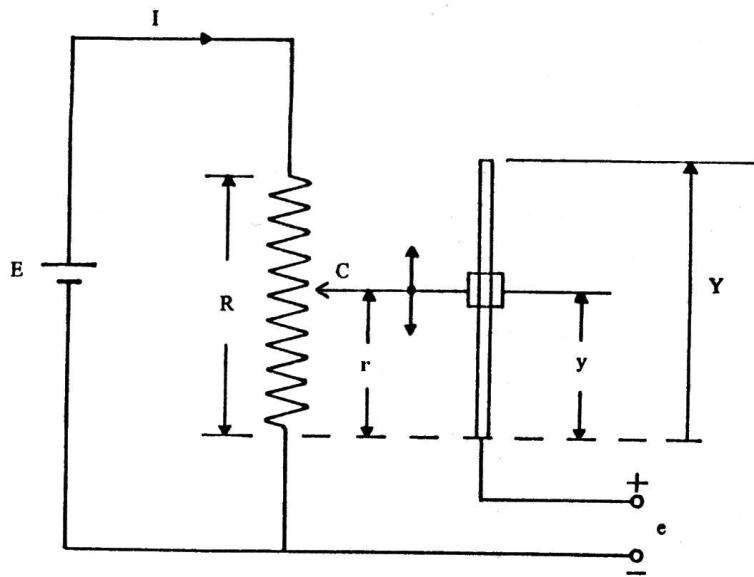
\includegraphics[width=0.4\linewidth]{fig/imag}

		\label{fig:imag}
	\end{figure}	
	\[V(0) = 0 \hspace{1cm} V(L) = E\]
	\[ \begin{cases}
		E = IR \\
		e = rI
	\end{cases} \Rightarrow \dfrac{e}{E} = \dfrac{r}{R} \]
	\[ R = \rho \dfrac{L}{S} \hspace{1cm} r = \rho \dfrac{x}{S}  \]
	\[ \dfrac{r}{R} = \dfrac{x}{L}\]
	Infine: 
	\[ \dfrac{e}{E} = \dfrac{x}{L} \]
	\[ e(t) = \dfrac{E}{L}x(t) \]
	Il potenziometro è in prima approssimazione uno strumento di ordine $0$, perché in prima approssimazione? In realtà il palpatore $C$ ha una sua ben definita massa, e quindi possiede inevitabilmente un'inerzia.  
\end{adjustwidth}
\newpage
\section{Strumento di ordine $I$}
\begin{adjustwidth}{2in}{}	
	\textbf{bilancia/dinamometro/termometro} 
	\begin{figure}[H]
		\centering
		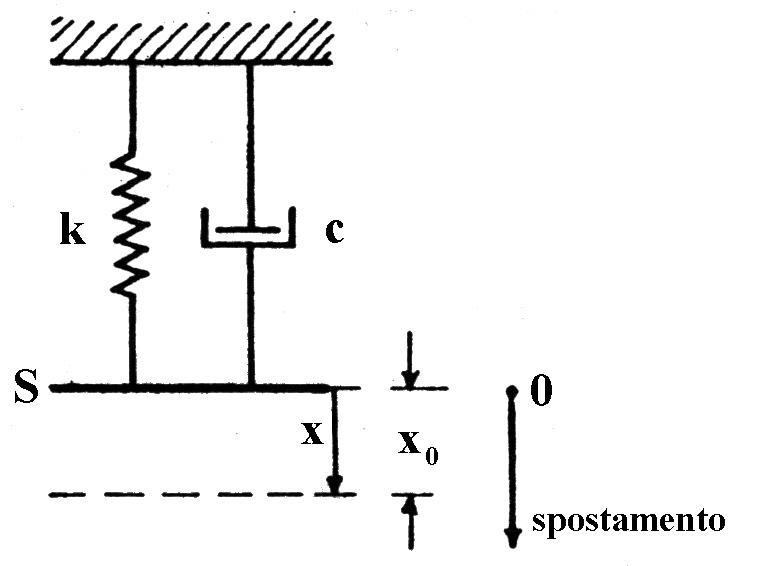
\includegraphics[width=0.5\linewidth]{fig/imag1}
		\label{fig:imag1}
	\end{figure}	
	In questo caso lo spostamento che misuro ($y$), è funzione della forza che applico ($F$):
	\[ ky + c\dot{y} = F(t)\]
	
	\begin{center}
		\textbf{È necessario risolvere le uscite per ogni ingresso}
	\end{center}
\end{adjustwidth}
%\newpage
\subsection{Gradino decrescente} 	
\begin{adjustwidth}{2in}{}
	Applico all'elemento una forza $F_0$, lo rilascio immediatamente e questa compie un gradino decrescente:
	\[ F(t) = \begin{cases}
		F_0 ~~ t \leq 0 \\
		0 ~~ t>0
	\end{cases}\]
	Risolvo la funzione all'esterno del gradino, per $t>0$, è lì che desidero tracciarne l'andamento, dopo quanto tempo la misura si adegua al nuovo input? 
	\[ ky + c\dot{y} = 0 \hspace{1cm} y(0) = \dfrac{F_0}{k}\]
	La soluzione generale è da ricercarsi nella forma: 
	\[  y(t) = Ae^{\alpha t}\]
	Per cui, sostituendo nell'equazione di partenza: 
	\[ kAe^{\alpha t} + c\alpha Ae^{\alpha t} = 0 \]
	\[ k + c\alpha  = 0 \]
	\[ \alpha  = -\dfrac{k}{c} = [ 1/s ]  \]
	Chiamo costante di tempo:
	\[ \tau = \dfrac{c}{k} = [ s ] \]
	In modo che: 
	\[  y(t) = Ae^{-t/\tau}\]
	Applicando la condizione iniziale si arriva ad una soluzione:
	\[  y(t) = \dfrac{F_0}{k}e^{-t/\tau}\]	
\begin{figure}[H]
	\centering
	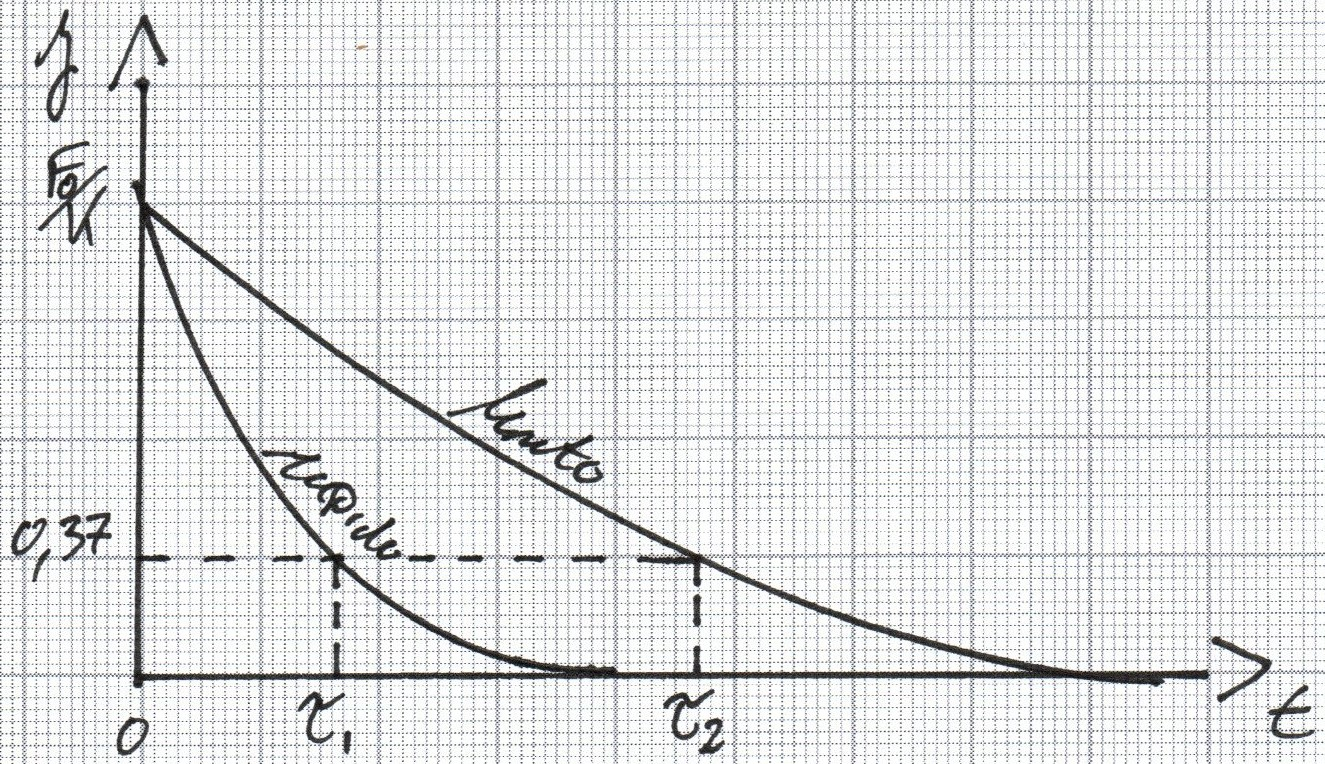
\includegraphics[width=0.4\linewidth]{fig/mm4}
	\label{fig:mm4}
\end{figure}
	Si noti che dopo un $\tau$:
	\[  y(\tau) = \dfrac{F_0}{k}e^{-1} = 0.37\dfrac{F_0}{k} \]
	Ho raggiunto il $37\%$ del valore iniziale.  
\end{adjustwidth}
%\newpage
\subsubsection{Metodo delle sottotangenti per la determinazione del $\tau$} 	
\begin{adjustwidth}{2in}{}	
	Derivo nel tempo il risultato appena ottenuto:
	\[  \dot{y}(t) = -\dfrac{1}{\tau} \dfrac{F_0}{k}e^{-t/\tau}\]
	Ma cos'è la derivata di una curva se non la retta tangente alla curva stessa? 	
\definecolor{ccqqqq}{rgb}{0.8,0.,0.}
\definecolor{qqwuqq}{rgb}{0.,0.39215686274509803,0.}
\begin{figure}[H]
	\centering
	\subfloat{\begin{tikzpicture}[line cap=round,line join=round,>=triangle 45]
			\begin{axis}[
				x=5cm,y=5cm,
				axis lines=middle,
				%					ymajorgrids=true,
				%					xmajorgrids=true,
				xmin=-0.18,
				xmax=1.85,
				ymin=0,
				ymax=1.45,
				ytick=\empty, xtick=\empty,
				xticklabels=\empty,yticklabels=\empty,extra x ticks={0,1}, extra y ticks={1},
				xlabel=$x$, ylabel=$y$]
				\clip(-0.2,-0.1) rectangle (1.8,1.4);
				%%%%%%%%%%%%%%%%%%%% ESPONENZIALE
				\draw[line width=2.pt,color=qqwuqq] (-0.2,1.2214027581601699) -- (-0.2,1.2214027581601699);
				\draw[line width=2.pt,color=qqwuqq] (-0.2,1.2214027581601699) -- (-0.195,1.2153109864897307);
				\draw[line width=2.pt,color=qqwuqq] (-0.195,1.2153109864897307) -- (-0.19,1.2092495976572515);
				\draw[line width=2.pt,color=qqwuqq] (-0.19,1.2092495976572515) -- (-0.185,1.2032184401276953);
				\draw[line width=2.pt,color=qqwuqq] (-0.185,1.2032184401276953) -- (-0.18,1.1972173631218102);
				\draw[line width=2.pt,color=qqwuqq] (-0.18,1.1972173631218102) -- (-0.175,1.191246216612358);
				\draw[line width=2.pt,color=qqwuqq] (-0.175,1.191246216612358) -- (-0.16999999999999998,1.1853048513203654);
				\draw[line width=2.pt,color=qqwuqq] (-0.16999999999999998,1.1853048513203654) -- (-0.16499999999999998,1.1793931187113906);
				\draw[line width=2.pt,color=qqwuqq] (-0.16499999999999998,1.1793931187113906) -- (-0.15999999999999998,1.1735108709918103);
				\draw[line width=2.pt,color=qqwuqq] (-0.15999999999999998,1.1735108709918103) -- (-0.15499999999999997,1.167657961105125);
				\draw[line width=2.pt,color=qqwuqq] (-0.15499999999999997,1.167657961105125) -- (-0.14999999999999997,1.161834242728283);
				\draw[line width=2.pt,color=qqwuqq] (-0.14999999999999997,1.161834242728283) -- (-0.14499999999999996,1.1560395702680215);
				\draw[line width=2.pt,color=qqwuqq] (-0.14499999999999996,1.1560395702680215) -- (-0.13999999999999996,1.1502737988572271);
				\draw[line width=2.pt,color=qqwuqq] (-0.13999999999999996,1.1502737988572271) -- (-0.13499999999999995,1.1445367843513143);
				\draw[line width=2.pt,color=qqwuqq] (-0.13499999999999995,1.1445367843513143) -- (-0.12999999999999995,1.1388283833246218);
				\draw[line width=2.pt,color=qqwuqq] (-0.12999999999999995,1.1388283833246218) -- (-0.12499999999999994,1.1331484530668263);
				\draw[line width=2.pt,color=qqwuqq] (-0.12499999999999994,1.1331484530668263) -- (-0.11999999999999994,1.1274968515793755);
				\draw[line width=2.pt,color=qqwuqq] (-0.11999999999999994,1.1274968515793755) -- (-0.11499999999999994,1.1218734375719384);
				\draw[line width=2.pt,color=qqwuqq] (-0.11499999999999994,1.1218734375719384) -- (-0.10999999999999993,1.1162780704588713);
				\draw[line width=2.pt,color=qqwuqq] (-0.10999999999999993,1.1162780704588713) -- (-0.10499999999999993,1.1107106103557052);
				\draw[line width=2.pt,color=qqwuqq] (-0.10499999999999993,1.1107106103557052) -- (-0.09999999999999992,1.1051709180756475);
				\draw[line width=2.pt,color=qqwuqq] (-0.09999999999999992,1.1051709180756475) -- (-0.09499999999999992,1.0996588551261028);
				\draw[line width=2.pt,color=qqwuqq] (-0.09499999999999992,1.0996588551261028) -- (-0.08999999999999991,1.0941742837052102);
				\draw[line width=2.pt,color=qqwuqq] (-0.08999999999999991,1.0941742837052102) -- (-0.08499999999999991,1.0887170666983985);
				\draw[line width=2.pt,color=qqwuqq] (-0.08499999999999991,1.0887170666983985) -- (-0.0799999999999999,1.0832870676749584);
				\draw[line width=2.pt,color=qqwuqq] (-0.0799999999999999,1.0832870676749584) -- (-0.0749999999999999,1.0778841508846315);
				\draw[line width=2.pt,color=qqwuqq] (-0.0749999999999999,1.0778841508846315) -- (-0.0699999999999999,1.0725081812542163);
				\draw[line width=2.pt,color=qqwuqq] (-0.0699999999999999,1.0725081812542163) -- (-0.06499999999999989,1.0671590243841924);
				\draw[line width=2.pt,color=qqwuqq] (-0.06499999999999989,1.0671590243841924) -- (-0.059999999999999894,1.0618365465453594);
				\draw[line width=2.pt,color=qqwuqq] (-0.059999999999999894,1.0618365465453594) -- (-0.054999999999999896,1.056540614675494);
				\draw[line width=2.pt,color=qqwuqq] (-0.054999999999999896,1.056540614675494) -- (-0.0499999999999999,1.051271096376024);
				\draw[line width=2.pt,color=qqwuqq] (-0.0499999999999999,1.051271096376024) -- (-0.0449999999999999,1.046027859908717);
				\draw[line width=2.pt,color=qqwuqq] (-0.0449999999999999,1.046027859908717) -- (-0.039999999999999904,1.0408107741923882);
				\draw[line width=2.pt,color=qqwuqq] (-0.039999999999999904,1.0408107741923882) -- (-0.034999999999999906,1.035619708799623);
				\draw[line width=2.pt,color=qqwuqq] (-0.034999999999999906,1.035619708799623) -- (-0.029999999999999905,1.0304545339535167);
				\draw[line width=2.pt,color=qqwuqq] (-0.029999999999999905,1.0304545339535167) -- (-0.024999999999999904,1.0253151205244286);
				\draw[line width=2.pt,color=qqwuqq] (-0.024999999999999904,1.0253151205244286) -- (-0.019999999999999903,1.0202013400267558);
				\draw[line width=2.pt,color=qqwuqq] (-0.019999999999999903,1.0202013400267558) -- (-0.014999999999999902,1.015113064615719);
				\draw[line width=2.pt,color=qqwuqq] (-0.014999999999999902,1.015113064615719) -- (-0.009999999999999901,1.010050167084168);
				\draw[line width=2.pt,color=qqwuqq] (-0.009999999999999901,1.010050167084168) -- (-0.004999999999999901,1.005012520859401);
				\draw[line width=2.pt,color=qqwuqq] (-0.004999999999999901,1.005012520859401) -- (0.0,0.9999999999999999);
				\draw[line width=2.pt,color=qqwuqq] (0.0,0.9999999999999999) -- (0.005000000000000099,0.9950124791926822);
				\draw[line width=2.pt,color=qqwuqq] (0.005000000000000099,0.9950124791926822) -- (0.010000000000000099,0.990049833749168);
				\draw[line width=2.pt,color=qqwuqq] (0.010000000000000099,0.990049833749168) -- (0.0150000000000001,0.9851119396030625);
				\draw[line width=2.pt,color=qqwuqq] (0.0150000000000001,0.9851119396030625) -- (0.0200000000000001,0.9801986733067553);
				\draw[line width=2.pt,color=qqwuqq] (0.0200000000000001,0.9801986733067553) -- (0.025000000000000102,0.9753099120283326);
				\draw[line width=2.pt,color=qqwuqq] (0.025000000000000102,0.9753099120283326) -- (0.030000000000000103,0.970445533548508);
				\draw[line width=2.pt,color=qqwuqq] (0.030000000000000103,0.970445533548508) -- (0.0350000000000001,0.9656054162575664);
				\draw[line width=2.pt,color=qqwuqq] (0.0350000000000001,0.9656054162575664) -- (0.0400000000000001,0.9607894391523231);
				\draw[line width=2.pt,color=qqwuqq] (0.0400000000000001,0.9607894391523231) -- (0.045000000000000095,0.9559974818330998);
				\draw[line width=2.pt,color=qqwuqq] (0.045000000000000095,0.9559974818330998) -- (0.05000000000000009,0.9512294245007139);
				\draw[line width=2.pt,color=qqwuqq] (0.05000000000000009,0.9512294245007139) -- (0.05500000000000009,0.9464851479534838);
				\draw[line width=2.pt,color=qqwuqq] (0.05500000000000009,0.9464851479534838) -- (0.06000000000000009,0.9417645335842486);
				\draw[line width=2.pt,color=qqwuqq] (0.06000000000000009,0.9417645335842486) -- (0.06500000000000009,0.9370674633774033);
				\draw[line width=2.pt,color=qqwuqq] (0.06500000000000009,0.9370674633774033) -- (0.07000000000000009,0.9323938199059482);
				\draw[line width=2.pt,color=qqwuqq] (0.07000000000000009,0.9323938199059482) -- (0.0750000000000001,0.9277434863285529);
				\draw[line width=2.pt,color=qqwuqq] (0.0750000000000001,0.9277434863285529) -- (0.0800000000000001,0.9231163463866356);
				\draw[line width=2.pt,color=qqwuqq] (0.0800000000000001,0.9231163463866356) -- (0.0850000000000001,0.9185122844014573);
				\draw[line width=2.pt,color=qqwuqq] (0.0850000000000001,0.9185122844014573) -- (0.09000000000000011,0.9139311852712281);
				\draw[line width=2.pt,color=qqwuqq] (0.09000000000000011,0.9139311852712281) -- (0.09500000000000011,0.9093729344682313);
				\draw[line width=2.pt,color=qqwuqq] (0.09500000000000011,0.9093729344682313) -- (0.10000000000000012,0.9048374180359595);
				\draw[line width=2.pt,color=qqwuqq] (0.10000000000000012,0.9048374180359595) -- (0.10500000000000012,0.9003245225862655);
				\draw[line width=2.pt,color=qqwuqq] (0.10500000000000012,0.9003245225862655) -- (0.11000000000000013,0.8958341352965281);
				\draw[line width=2.pt,color=qqwuqq] (0.11000000000000013,0.8958341352965281) -- (0.11500000000000013,0.8913661439068312);
				\draw[line width=2.pt,color=qqwuqq] (0.11500000000000013,0.8913661439068312) -- (0.12000000000000013,0.8869204367171574);
				\draw[line width=2.pt,color=qqwuqq] (0.12000000000000013,0.8869204367171574) -- (0.12500000000000014,0.8824969025845952);
				\draw[line width=2.pt,color=qqwuqq] (0.12500000000000014,0.8824969025845952) -- (0.13000000000000014,0.8780954309205612);
				\draw[line width=2.pt,color=qqwuqq] (0.13000000000000014,0.8780954309205612) -- (0.13500000000000015,0.8737159116880343);
				\draw[line width=2.pt,color=qqwuqq] (0.13500000000000015,0.8737159116880343) -- (0.14000000000000015,0.8693582353988057);
				\draw[line width=2.pt,color=qqwuqq] (0.14000000000000015,0.8693582353988057) -- (0.14500000000000016,0.8650222931107412);
				\draw[line width=2.pt,color=qqwuqq] (0.14500000000000016,0.8650222931107412) -- (0.15000000000000016,0.8607079764250577);
				\draw[line width=2.pt,color=qqwuqq] (0.15000000000000016,0.8607079764250577) -- (0.15500000000000017,0.8564151774836134);
				\draw[line width=2.pt,color=qqwuqq] (0.15500000000000017,0.8564151774836134) -- (0.16000000000000017,0.8521437889662112);
				\draw[line width=2.pt,color=qqwuqq] (0.16000000000000017,0.8521437889662112) -- (0.16500000000000017,0.8478937040879156);
				\draw[line width=2.pt,color=qqwuqq] (0.16500000000000017,0.8478937040879156) -- (0.17000000000000018,0.8436648165963836);
				\draw[line width=2.pt,color=qqwuqq] (0.17000000000000018,0.8436648165963836) -- (0.17500000000000018,0.8394570207692073);
				\draw[line width=2.pt,color=qqwuqq] (0.17500000000000018,0.8394570207692073) -- (0.1800000000000002,0.8352702114112719);
				\draw[line width=2.pt,color=qqwuqq] (0.1800000000000002,0.8352702114112719) -- (0.1850000000000002,0.8311042838521255);
				\draw[line width=2.pt,color=qqwuqq] (0.1850000000000002,0.8311042838521255) -- (0.1900000000000002,0.8269591339433622);
				\draw[line width=2.pt,color=qqwuqq] (0.1900000000000002,0.8269591339433622) -- (0.1950000000000002,0.8228346580560182);
				\draw[line width=2.pt,color=qqwuqq] (0.1950000000000002,0.8228346580560182) -- (0.2000000000000002,0.8187307530779817);
				\draw[line width=2.pt,color=qqwuqq] (0.2000000000000002,0.8187307530779817) -- (0.2050000000000002,0.8146473164114144);
				\draw[line width=2.pt,color=qqwuqq] (0.2050000000000002,0.8146473164114144) -- (0.21000000000000021,0.810584245970187);
				\draw[line width=2.pt,color=qqwuqq] (0.21000000000000021,0.810584245970187) -- (0.21500000000000022,0.8065414401773267);
				\draw[line width=2.pt,color=qqwuqq] (0.21500000000000022,0.8065414401773267) -- (0.22000000000000022,0.8025187979624783);
				\draw[line width=2.pt,color=qqwuqq] (0.22000000000000022,0.8025187979624783) -- (0.22500000000000023,0.7985162187593768);
				\draw[line width=2.pt,color=qqwuqq] (0.22500000000000023,0.7985162187593768) -- (0.23000000000000023,0.7945336025033338);
				\draw[line width=2.pt,color=qqwuqq] (0.23000000000000023,0.7945336025033338) -- (0.23500000000000024,0.7905708496287354);
				\draw[line width=2.pt,color=qqwuqq] (0.23500000000000024,0.7905708496287354) -- (0.24000000000000024,0.7866278610665532);
				\draw[line width=2.pt,color=qqwuqq] (0.24000000000000024,0.7866278610665532) -- (0.24500000000000025,0.782704538241868);
				\draw[line width=2.pt,color=qqwuqq] (0.24500000000000025,0.782704538241868) -- (0.2500000000000002,0.7788007830714047);
				\draw[line width=2.pt,color=qqwuqq] (0.2500000000000002,0.7788007830714047) -- (0.2550000000000002,0.7749164979610808);
				\draw[line width=2.pt,color=qqwuqq] (0.2550000000000002,0.7749164979610808) -- (0.26000000000000023,0.7710515858035661);
				\draw[line width=2.pt,color=qqwuqq] (0.26000000000000023,0.7710515858035661) -- (0.26500000000000024,0.7672059499758556);
				\draw[line width=2.pt,color=qqwuqq] (0.26500000000000024,0.7672059499758556) -- (0.27000000000000024,0.763379494336853);
				\draw[line width=2.pt,color=qqwuqq] (0.27000000000000024,0.763379494336853) -- (0.27500000000000024,0.7595721232249683);
				\draw[line width=2.pt,color=qqwuqq] (0.27500000000000024,0.7595721232249683) -- (0.28000000000000025,0.7557837414557252);
				\draw[line width=2.pt,color=qqwuqq] (0.28000000000000025,0.7557837414557252) -- (0.28500000000000025,0.7520142543193824);
				\draw[line width=2.pt,color=qqwuqq] (0.28500000000000025,0.7520142543193824) -- (0.29000000000000026,0.748263567578565);
				\draw[line width=2.pt,color=qqwuqq] (0.29000000000000026,0.748263567578565) -- (0.29500000000000026,0.7445315874659092);
				\draw[line width=2.pt,color=qqwuqq] (0.29500000000000026,0.7445315874659092) -- (0.30000000000000027,0.7408182206817177);
				\draw[line width=2.pt,color=qqwuqq] (0.30000000000000027,0.7408182206817177) -- (0.30500000000000027,0.7371233743916276);
				\draw[line width=2.pt,color=qqwuqq] (0.30500000000000027,0.7371233743916276) -- (0.3100000000000003,0.7334469562242891);
				\draw[line width=2.pt,color=qqwuqq] (0.3100000000000003,0.7334469562242891) -- (0.3150000000000003,0.7297888742690566);
				\draw[line width=2.pt,color=qqwuqq] (0.3150000000000003,0.7297888742690566) -- (0.3200000000000003,0.7261490370736907);
				\draw[line width=2.pt,color=qqwuqq] (0.3200000000000003,0.7261490370736907) -- (0.3250000000000003,0.722527353642072);
				\draw[line width=2.pt,color=qqwuqq] (0.3250000000000003,0.722527353642072) -- (0.3300000000000003,0.718923733431926);
				\draw[line width=2.pt,color=qqwuqq] (0.3300000000000003,0.718923733431926) -- (0.3350000000000003,0.7153380863525597);
				\draw[line width=2.pt,color=qqwuqq] (0.3350000000000003,0.7153380863525597) -- (0.3400000000000003,0.7117703227626095);
				\draw[line width=2.pt,color=qqwuqq] (0.3400000000000003,0.7117703227626095) -- (0.3450000000000003,0.7082203534677998);
				\draw[line width=2.pt,color=qqwuqq] (0.3450000000000003,0.7082203534677998) -- (0.3500000000000003,0.7046880897187132);
				\draw[line width=2.pt,color=qqwuqq] (0.3500000000000003,0.7046880897187132) -- (0.3550000000000003,0.7011734432085722);
				\draw[line width=2.pt,color=qqwuqq] (0.3550000000000003,0.7011734432085722) -- (0.3600000000000003,0.6976763260710308);
				\draw[line width=2.pt,color=qqwuqq] (0.3600000000000003,0.6976763260710308) -- (0.3650000000000003,0.6941966508779787);
				\draw[line width=2.pt,color=qqwuqq] (0.3650000000000003,0.6941966508779787) -- (0.37000000000000033,0.6907343306373545);
				\draw[line width=2.pt,color=qqwuqq] (0.37000000000000033,0.6907343306373545) -- (0.37500000000000033,0.687289278790972);
				\draw[line width=2.pt,color=qqwuqq] (0.37500000000000033,0.687289278790972) -- (0.38000000000000034,0.6838614092123556);
				\draw[line width=2.pt,color=qqwuqq] (0.38000000000000034,0.6838614092123556) -- (0.38500000000000034,0.6804506362045875);
				\draw[line width=2.pt,color=qqwuqq] (0.38500000000000034,0.6804506362045875) -- (0.39000000000000035,0.6770568744981644);
				\draw[line width=2.pt,color=qqwuqq] (0.39000000000000035,0.6770568744981644) -- (0.39500000000000035,0.6736800392488674);
				\draw[line width=2.pt,color=qqwuqq] (0.39500000000000035,0.6736800392488674) -- (0.40000000000000036,0.6703200460356391);
				\draw[line width=2.pt,color=qqwuqq] (0.40000000000000036,0.6703200460356391) -- (0.40500000000000036,0.6669768108584742);
				\draw[line width=2.pt,color=qqwuqq] (0.40500000000000036,0.6669768108584742) -- (0.41000000000000036,0.6636502501363192);
				\draw[line width=2.pt,color=qqwuqq] (0.41000000000000036,0.6636502501363192) -- (0.41500000000000037,0.6603402807049826);
				\draw[line width=2.pt,color=qqwuqq] (0.41500000000000037,0.6603402807049826) -- (0.4200000000000004,0.6570468198150565);
				\draw[line width=2.pt,color=qqwuqq] (0.4200000000000004,0.6570468198150565) -- (0.4250000000000004,0.6537697851298471);
				\draw[line width=2.pt,color=qqwuqq] (0.4250000000000004,0.6537697851298471) -- (0.4300000000000004,0.6505090947233163);
				\draw[line width=2.pt,color=qqwuqq] (0.4300000000000004,0.6505090947233163) -- (0.4350000000000004,0.6472646670780344);
				\draw[line width=2.pt,color=qqwuqq] (0.4350000000000004,0.6472646670780344) -- (0.4400000000000004,0.6440364210831411);
				\draw[line width=2.pt,color=qqwuqq] (0.4400000000000004,0.6440364210831411) -- (0.4450000000000004,0.6408242760323185);
				\draw[line width=2.pt,color=qqwuqq] (0.4450000000000004,0.6408242760323185) -- (0.4500000000000004,0.637628151621773);
				\draw[line width=2.pt,color=qqwuqq] (0.4500000000000004,0.637628151621773) -- (0.4550000000000004,0.6344479679482279);
				\draw[line width=2.pt,color=qqwuqq] (0.4550000000000004,0.6344479679482279) -- (0.4600000000000004,0.6312836455069257);
				\draw[line width=2.pt,color=qqwuqq] (0.4600000000000004,0.6312836455069257) -- (0.4650000000000004,0.6281351051896406);
				\draw[line width=2.pt,color=qqwuqq] (0.4650000000000004,0.6281351051896406) -- (0.4700000000000004,0.6250022682827006);
				\draw[line width=2.pt,color=qqwuqq] (0.4700000000000004,0.6250022682827006) -- (0.4750000000000004,0.6218850564650198);
				\draw[line width=2.pt,color=qqwuqq] (0.4750000000000004,0.6218850564650198) -- (0.4800000000000004,0.6187833918061406);
				\draw[line width=2.pt,color=qqwuqq] (0.4800000000000004,0.6187833918061406) -- (0.48500000000000043,0.6156971967642849);
				\draw[line width=2.pt,color=qqwuqq] (0.48500000000000043,0.6156971967642849) -- (0.49000000000000044,0.6126263941844158);
				\draw[line width=2.pt,color=qqwuqq] (0.49000000000000044,0.6126263941844158) -- (0.49500000000000044,0.609570907296309);
				\draw[line width=2.pt,color=qqwuqq] (0.49500000000000044,0.609570907296309) -- (0.5000000000000004,0.6065306597126332);
				\draw[line width=2.pt,color=qqwuqq] (0.5000000000000004,0.6065306597126332) -- (0.5050000000000004,0.6035055754270403);
				\draw[line width=2.pt,color=qqwuqq] (0.5050000000000004,0.6035055754270403) -- (0.5100000000000005,0.6004955788122657);
				\draw[line width=2.pt,color=qqwuqq] (0.5100000000000005,0.6004955788122657) -- (0.5150000000000005,0.5975005946182372);
				\draw[line width=2.pt,color=qqwuqq] (0.5150000000000005,0.5975005946182372) -- (0.5200000000000005,0.594520547970194);
				\draw[line width=2.pt,color=qqwuqq] (0.5200000000000005,0.594520547970194) -- (0.5250000000000005,0.5915553643668148);
				\draw[line width=2.pt,color=qqwuqq] (0.5250000000000005,0.5915553643668148) -- (0.5300000000000005,0.588604969678355);
				\draw[line width=2.pt,color=qqwuqq] (0.5300000000000005,0.588604969678355) -- (0.5350000000000005,0.5856692901447935);
				\draw[line width=2.pt,color=qqwuqq] (0.5350000000000005,0.5856692901447935) -- (0.5400000000000005,0.5827482523739894);
				\draw[line width=2.pt,color=qqwuqq] (0.5400000000000005,0.5827482523739894) -- (0.5450000000000005,0.5798417833398462);
				\draw[line width=2.pt,color=qqwuqq] (0.5450000000000005,0.5798417833398462) -- (0.5500000000000005,0.5769498103804864);
				\draw[line width=2.pt,color=qqwuqq] (0.5500000000000005,0.5769498103804864) -- (0.5550000000000005,0.5740722611964357);
				\draw[line width=2.pt,color=qqwuqq] (0.5550000000000005,0.5740722611964357) -- (0.5600000000000005,0.5712090638488146);
				\draw[line width=2.pt,color=qqwuqq] (0.5600000000000005,0.5712090638488146) -- (0.5650000000000005,0.5683601467575402);
				\draw[line width=2.pt,color=qqwuqq] (0.5650000000000005,0.5683601467575402) -- (0.5700000000000005,0.5655254386995369);
				\draw[line width=2.pt,color=qqwuqq] (0.5700000000000005,0.5655254386995369) -- (0.5750000000000005,0.5627048688069555);
				\draw[line width=2.pt,color=qqwuqq] (0.5750000000000005,0.5627048688069555) -- (0.5800000000000005,0.5598983665654017);
				\draw[line width=2.pt,color=qqwuqq] (0.5800000000000005,0.5598983665654017) -- (0.5850000000000005,0.5571058618121736);
				\draw[line width=2.pt,color=qqwuqq] (0.5850000000000005,0.5571058618121736) -- (0.5900000000000005,0.5543272847345068);
				\draw[line width=2.pt,color=qqwuqq] (0.5900000000000005,0.5543272847345068) -- (0.5950000000000005,0.5515625658678295);
				\draw[line width=2.pt,color=qqwuqq] (0.5950000000000005,0.5515625658678295) -- (0.6000000000000005,0.5488116360940262);
				\draw[line width=2.pt,color=qqwuqq] (0.6000000000000005,0.5488116360940262) -- (0.6050000000000005,0.5460744266397092);
				\draw[line width=2.pt,color=qqwuqq] (0.6050000000000005,0.5460744266397092) -- (0.6100000000000005,0.5433508690744995);
				\draw[line width=2.pt,color=qqwuqq] (0.6100000000000005,0.5433508690744995) -- (0.6150000000000005,0.5406408953093162);
				\draw[line width=2.pt,color=qqwuqq] (0.6150000000000005,0.5406408953093162) -- (0.6200000000000006,0.5379444375946743);
				\draw[line width=2.pt,color=qqwuqq] (0.6200000000000006,0.5379444375946743) -- (0.6250000000000006,0.53526142851899);
				\draw[line width=2.pt,color=qqwuqq] (0.6250000000000006,0.53526142851899) -- (0.6300000000000006,0.532591801006897);
				\draw[line width=2.pt,color=qqwuqq] (0.6300000000000006,0.532591801006897) -- (0.6350000000000006,0.5299354883175682);
				\draw[line width=2.pt,color=qqwuqq] (0.6350000000000006,0.5299354883175682) -- (0.6400000000000006,0.5272924240430483);
				\draw[line width=2.pt,color=qqwuqq] (0.6400000000000006,0.5272924240430483) -- (0.6450000000000006,0.5246625421065926);
				\draw[line width=2.pt,color=qqwuqq] (0.6450000000000006,0.5246625421065926) -- (0.6500000000000006,0.5220457767610157);
				\draw[line width=2.pt,color=qqwuqq] (0.6500000000000006,0.5220457767610157) -- (0.6550000000000006,0.5194420625870478);
				\draw[line width=2.pt,color=qqwuqq] (0.6550000000000006,0.5194420625870478) -- (0.6600000000000006,0.516851334491699);
				\draw[line width=2.pt,color=qqwuqq] (0.6600000000000006,0.516851334491699) -- (0.6650000000000006,0.5142735277066317);
				\draw[line width=2.pt,color=qqwuqq] (0.6650000000000006,0.5142735277066317) -- (0.6700000000000006,0.5117085777865422);
				\draw[line width=2.pt,color=qqwuqq] (0.6700000000000006,0.5117085777865422) -- (0.6750000000000006,0.5091564206075488);
				\draw[line width=2.pt,color=qqwuqq] (0.6750000000000006,0.5091564206075488) -- (0.6800000000000006,0.5066169923655893);
				\draw[line width=2.pt,color=qqwuqq] (0.6800000000000006,0.5066169923655893) -- (0.6850000000000006,0.5040902295748252);
				\draw[line width=2.pt,color=qqwuqq] (0.6850000000000006,0.5040902295748252) -- (0.6900000000000006,0.5015760690660552);
				\draw[line width=2.pt,color=qqwuqq] (0.6900000000000006,0.5015760690660552) -- (0.6950000000000006,0.49907444798513567);
				\draw[line width=2.pt,color=qqwuqq] (0.6950000000000006,0.49907444798513567) -- (0.7000000000000006,0.49658530379140925);
				\draw[line width=2.pt,color=qqwuqq] (0.7000000000000006,0.49658530379140925) -- (0.7050000000000006,0.4941085742561414);
				\draw[line width=2.pt,color=qqwuqq] (0.7050000000000006,0.4941085742561414) -- (0.7100000000000006,0.4916441974609648);
				\draw[line width=2.pt,color=qqwuqq] (0.7100000000000006,0.4916441974609648) -- (0.7150000000000006,0.48919211179633126);
				\draw[line width=2.pt,color=qqwuqq] (0.7150000000000006,0.48919211179633126) -- (0.7200000000000006,0.48675225595997135);
				\draw[line width=2.pt,color=qqwuqq] (0.7200000000000006,0.48675225595997135) -- (0.7250000000000006,0.4843245689553622);
				\draw[line width=2.pt,color=qqwuqq] (0.7250000000000006,0.4843245689553622) -- (0.7300000000000006,0.48190899009020216);
				\draw[line width=2.pt,color=qqwuqq] (0.7300000000000006,0.48190899009020216) -- (0.7350000000000007,0.4795054589748938);
				\draw[line width=2.pt,color=qqwuqq] (0.7350000000000007,0.4795054589748938) -- (0.7400000000000007,0.4771139155210341);
				\draw[line width=2.pt,color=qqwuqq] (0.7400000000000007,0.4771139155210341) -- (0.7450000000000007,0.4747342999399121);
				\draw[line width=2.pt,color=qqwuqq] (0.7450000000000007,0.4747342999399121) -- (0.7500000000000007,0.4723665527410144);
				\draw[line width=2.pt,color=qqwuqq] (0.7500000000000007,0.4723665527410144) -- (0.7550000000000007,0.4700106147305377);
				\draw[line width=2.pt,color=qqwuqq] (0.7550000000000007,0.4700106147305377) -- (0.7600000000000007,0.46766642700990896);
				\draw[line width=2.pt,color=qqwuqq] (0.7600000000000007,0.46766642700990896) -- (0.7650000000000007,0.4653339309743131);
				\draw[line width=2.pt,color=qqwuqq] (0.7650000000000007,0.4653339309743131) -- (0.7700000000000007,0.4630130683112278);
				\draw[line width=2.pt,color=qqwuqq] (0.7700000000000007,0.4630130683112278) -- (0.7750000000000007,0.46070378099896553);
				\draw[line width=2.pt,color=qqwuqq] (0.7750000000000007,0.46070378099896553) -- (0.7800000000000007,0.45840601130522324);
				\draw[line width=2.pt,color=qqwuqq] (0.7800000000000007,0.45840601130522324) -- (0.7850000000000007,0.45611970178563893);
				\draw[line width=2.pt,color=qqwuqq] (0.7850000000000007,0.45611970178563893) -- (0.7900000000000007,0.4538447952823555);
				\draw[line width=2.pt,color=qqwuqq] (0.7900000000000007,0.4538447952823555) -- (0.7950000000000007,0.45158123492259195);
				\draw[line width=2.pt,color=qqwuqq] (0.7950000000000007,0.45158123492259195) -- (0.8000000000000007,0.4493289641172213);
				\draw[line width=2.pt,color=qqwuqq] (0.8000000000000007,0.4493289641172213) -- (0.8050000000000007,0.44708792655935614);
				\draw[line width=2.pt,color=qqwuqq] (0.8050000000000007,0.44708792655935614) -- (0.8100000000000007,0.44485806622294083);
				\draw[line width=2.pt,color=qqwuqq] (0.8100000000000007,0.44485806622294083) -- (0.8150000000000007,0.4426393273613508);
				\draw[line width=2.pt,color=qqwuqq] (0.8150000000000007,0.4426393273613508) -- (0.8200000000000007,0.44043165450599897);
				\draw[line width=2.pt,color=qqwuqq] (0.8200000000000007,0.44043165450599897) -- (0.8250000000000007,0.43823499246494896);
				\draw[line width=2.pt,color=qqwuqq] (0.8250000000000007,0.43823499246494896) -- (0.8300000000000007,0.4360492863215353);
				\draw[line width=2.pt,color=qqwuqq] (0.8300000000000007,0.4360492863215353) -- (0.8350000000000007,0.4338744814329906);
				\draw[line width=2.pt,color=qqwuqq] (0.8350000000000007,0.4338744814329906) -- (0.8400000000000007,0.4317105234290794);
				\draw[line width=2.pt,color=qqwuqq] (0.8400000000000007,0.4317105234290794) -- (0.8450000000000008,0.42955735821073887);
				\draw[line width=2.pt,color=qqwuqq] (0.8450000000000008,0.42955735821073887) -- (0.8500000000000008,0.4274149319487264);
				\draw[line width=2.pt,color=qqwuqq] (0.8500000000000008,0.4274149319487264) -- (0.8550000000000008,0.4252831910822738);
				\draw[line width=2.pt,color=qqwuqq] (0.8550000000000008,0.4252831910822738) -- (0.8600000000000008,0.4231620823177485);
				\draw[line width=2.pt,color=qqwuqq] (0.8600000000000008,0.4231620823177485) -- (0.8650000000000008,0.42105155262732086);
				\draw[line width=2.pt,color=qqwuqq] (0.8650000000000008,0.42105155262732086) -- (0.8700000000000008,0.41895154924763867);
				\draw[line width=2.pt,color=qqwuqq] (0.8700000000000008,0.41895154924763867) -- (0.8750000000000008,0.4168620196785081);
				\draw[line width=2.pt,color=qqwuqq] (0.8750000000000008,0.4168620196785081) -- (0.8800000000000008,0.41478291168158105);
				\draw[line width=2.pt,color=qqwuqq] (0.8800000000000008,0.41478291168158105) -- (0.8850000000000008,0.41271417327904936);
				\draw[line width=2.pt,color=qqwuqq] (0.8850000000000008,0.41271417327904936) -- (0.8900000000000008,0.41065575275234517);
				\draw[line width=2.pt,color=qqwuqq] (0.8900000000000008,0.41065575275234517) -- (0.8950000000000008,0.40860759864084817);
				\draw[line width=2.pt,color=qqwuqq] (0.8950000000000008,0.40860759864084817) -- (0.9000000000000008,0.40656965974059883);
				\draw[line width=2.pt,color=qqwuqq] (0.9000000000000008,0.40656965974059883) -- (0.9050000000000008,0.4045418851030185);
				\draw[line width=2.pt,color=qqwuqq] (0.9050000000000008,0.4045418851030185) -- (0.9100000000000008,0.4025242240336357);
				\draw[line width=2.pt,color=qqwuqq] (0.9100000000000008,0.4025242240336357) -- (0.9150000000000008,0.4005166260908185);
				\draw[line width=2.pt,color=qqwuqq] (0.9150000000000008,0.4005166260908185) -- (0.9200000000000008,0.39851904108451386);
				\draw[line width=2.pt,color=qqwuqq] (0.9200000000000008,0.39851904108451386) -- (0.9250000000000008,0.39653141907499256);
				\draw[line width=2.pt,color=qqwuqq] (0.9250000000000008,0.39653141907499256) -- (0.9300000000000008,0.3945537103716008);
				\draw[line width=2.pt,color=qqwuqq] (0.9300000000000008,0.3945537103716008) -- (0.9350000000000008,0.3925858655315181);
				\draw[line width=2.pt,color=qqwuqq] (0.9350000000000008,0.3925858655315181) -- (0.9400000000000008,0.3906278353585208);
				\draw[line width=2.pt,color=qqwuqq] (0.9400000000000008,0.3906278353585208) -- (0.9450000000000008,0.3886795709017527);
				\draw[line width=2.pt,color=qqwuqq] (0.9450000000000008,0.3886795709017527) -- (0.9500000000000008,0.3867410234545009);
				\draw[line width=2.pt,color=qqwuqq] (0.9500000000000008,0.3867410234545009) -- (0.9550000000000008,0.38481214455297824);
				\draw[line width=2.pt,color=qqwuqq] (0.9550000000000008,0.38481214455297824) -- (0.9600000000000009,0.38289288597511173);
				\draw[line width=2.pt,color=qqwuqq] (0.9600000000000009,0.38289288597511173) -- (0.9650000000000009,0.3809831997393369);
				\draw[line width=2.pt,color=qqwuqq] (0.9650000000000009,0.3809831997393369) -- (0.9700000000000009,0.3790830381033985);
				\draw[line width=2.pt,color=qqwuqq] (0.9700000000000009,0.3790830381033985) -- (0.9750000000000009,0.3771923535631566);
				\draw[line width=2.pt,color=qqwuqq] (0.9750000000000009,0.3771923535631566) -- (0.9800000000000009,0.37531109885139924);
				\draw[line width=2.pt,color=qqwuqq] (0.9800000000000009,0.37531109885139924) -- (0.9850000000000009,0.3734392269366606);
				\draw[line width=2.pt,color=qqwuqq] (0.9850000000000009,0.3734392269366606) -- (0.9900000000000009,0.3715766910220454);
				\draw[line width=2.pt,color=qqwuqq] (0.9900000000000009,0.3715766910220454) -- (0.9950000000000009,0.3697234445440587);
				\draw[line width=2.pt,color=qqwuqq] (0.9950000000000009,0.3697234445440587) -- (1.0000000000000009,0.367879441171442);
				\draw[line width=2.pt,color=qqwuqq] (1.0000000000000009,0.367879441171442) -- (1.0050000000000008,0.36604463480401506);
				\draw[line width=2.pt,color=qqwuqq] (1.0050000000000008,0.36604463480401506) -- (1.0100000000000007,0.3642189795715231);
				\draw[line width=2.pt,color=qqwuqq] (1.0100000000000007,0.3642189795715231) -- (1.0150000000000006,0.36240242983249016);
				\draw[line width=2.pt,color=qqwuqq] (1.0150000000000006,0.36240242983249016) -- (1.0200000000000005,0.36059494017307814);
				\draw[line width=2.pt,color=qqwuqq] (1.0200000000000005,0.36059494017307814) -- (1.0250000000000004,0.3587964654059515);
				\draw[line width=2.pt,color=qqwuqq] (1.0250000000000004,0.3587964654059515) -- (1.0300000000000002,0.3570069605691473);
				\draw[line width=2.pt,color=qqwuqq] (1.0300000000000002,0.3570069605691473) -- (1.0350000000000001,0.35522638092495146);
				\draw[line width=2.pt,color=qqwuqq] (1.0350000000000001,0.35522638092495146) -- (1.04,0.35345468195878016);
				\draw[line width=2.pt,color=qqwuqq] (1.04,0.35345468195878016) -- (1.045,0.3516918193780669);
				\draw[line width=2.pt,color=qqwuqq] (1.045,0.3516918193780669) -- (1.0499999999999998,0.34993774911115544);
				\draw[line width=2.pt,color=qqwuqq] (1.0499999999999998,0.34993774911115544) -- (1.0549999999999997,0.34819242730619765);
				\draw[line width=2.pt,color=qqwuqq] (1.0549999999999997,0.34819242730619765) -- (1.0599999999999996,0.34645581033005757);
				\draw[line width=2.pt,color=qqwuqq] (1.0599999999999996,0.34645581033005757) -- (1.0649999999999995,0.34472785476722034);
				\draw[line width=2.pt,color=qqwuqq] (1.0649999999999995,0.34472785476722034) -- (1.0699999999999994,0.3430085174187069);
				\draw[line width=2.pt,color=qqwuqq] (1.0699999999999994,0.3430085174187069) -- (1.0749999999999993,0.34129775530099393);
				\draw[line width=2.pt,color=qqwuqq] (1.0749999999999993,0.34129775530099393) -- (1.0799999999999992,0.33959552564493944);
				\draw[line width=2.pt,color=qqwuqq] (1.0799999999999992,0.33959552564493944) -- (1.084999999999999,0.33790178589471337);
				\draw[line width=2.pt,color=qqwuqq] (1.084999999999999,0.33790178589471337) -- (1.089999999999999,0.33621649370673373);
				\draw[line width=2.pt,color=qqwuqq] (1.089999999999999,0.33621649370673373) -- (1.0949999999999989,0.334539606948608);
				\draw[line width=2.pt,color=qqwuqq] (1.0949999999999989,0.334539606948608) -- (1.0999999999999988,0.33287108369808);
				\draw[line width=2.pt,color=qqwuqq] (1.0999999999999988,0.33287108369808) -- (1.1049999999999986,0.3312108822419815);
				\draw[line width=2.pt,color=qqwuqq] (1.1049999999999986,0.3312108822419815) -- (1.1099999999999985,0.32955896107518956);
				\draw[line width=2.pt,color=qqwuqq] (1.1099999999999985,0.32955896107518956) -- (1.1149999999999984,0.3279152788995891);
				\draw[line width=2.pt,color=qqwuqq] (1.1149999999999984,0.3279152788995891) -- (1.1199999999999983,0.32627979462304);
				\draw[line width=2.pt,color=qqwuqq] (1.1199999999999983,0.32627979462304) -- (1.1249999999999982,0.32465246735835035);
				\draw[line width=2.pt,color=qqwuqq] (1.1249999999999982,0.32465246735835035) -- (1.1299999999999981,0.32303325642225356);
				\draw[line width=2.pt,color=qqwuqq] (1.1299999999999981,0.32303325642225356) -- (1.134999999999998,0.321422121334392);
				\draw[line width=2.pt,color=qqwuqq] (1.134999999999998,0.321422121334392) -- (1.139999999999998,0.31981902181630456);
				\draw[line width=2.pt,color=qqwuqq] (1.139999999999998,0.31981902181630456) -- (1.1449999999999978,0.3182239177904198);
				\draw[line width=2.pt,color=qqwuqq] (1.1449999999999978,0.3182239177904198) -- (1.1499999999999977,0.316636769379054);
				\draw[line width=2.pt,color=qqwuqq] (1.1499999999999977,0.316636769379054) -- (1.1549999999999976,0.3150575369034141);
				\draw[line width=2.pt,color=qqwuqq] (1.1549999999999976,0.3150575369034141) -- (1.1599999999999975,0.3134861808826061);
				\draw[line width=2.pt,color=qqwuqq] (1.1599999999999975,0.3134861808826061) -- (1.1649999999999974,0.31192266203264757);
				\draw[line width=2.pt,color=qqwuqq] (1.1649999999999974,0.31192266203264757) -- (1.1699999999999973,0.31036694126548586);
				\draw[line width=2.pt,color=qqwuqq] (1.1699999999999973,0.31036694126548586) -- (1.1749999999999972,0.30881897968802074);
				\draw[line width=2.pt,color=qqwuqq] (1.1749999999999972,0.30881897968802074) -- (1.179999999999997,0.30727873860113214);
				\draw[line width=2.pt,color=qqwuqq] (1.179999999999997,0.30727873860113214) -- (1.184999999999997,0.3057461794987127);
				\draw[line width=2.pt,color=qqwuqq] (1.184999999999997,0.3057461794987127) -- (1.1899999999999968,0.304221264066705);
				\draw[line width=2.pt,color=qqwuqq] (1.1899999999999968,0.304221264066705) -- (1.1949999999999967,0.3027039541821439);
				\draw[line width=2.pt,color=qqwuqq] (1.1949999999999967,0.3027039541821439) -- (1.1999999999999966,0.30119421191220314);
				\draw[line width=2.pt,color=qqwuqq] (1.1999999999999966,0.30119421191220314) -- (1.2049999999999965,0.2996919995132474);
				\draw[line width=2.pt,color=qqwuqq] (1.2049999999999965,0.2996919995132474) -- (1.2099999999999964,0.29819727942988844);
				\draw[line width=2.pt,color=qqwuqq] (1.2099999999999964,0.29819727942988844) -- (1.2149999999999963,0.2967100142940464);
				\draw[line width=2.pt,color=qqwuqq] (1.2149999999999963,0.2967100142940464) -- (1.2199999999999962,0.2952301669240153);
				\draw[line width=2.pt,color=qqwuqq] (1.2199999999999962,0.2952301669240153) -- (1.224999999999996,0.293757700323534);
				\draw[line width=2.pt,color=qqwuqq] (1.224999999999996,0.293757700323534) -- (1.229999999999996,0.2922925776808606);
				\draw[line width=2.pt,color=qqwuqq] (1.229999999999996,0.2922925776808606) -- (1.2349999999999959,0.29083476236785283);
				\draw[line width=2.pt,color=qqwuqq] (1.2349999999999959,0.29083476236785283) -- (1.2399999999999958,0.2893842179390519);
				\draw[line width=2.pt,color=qqwuqq] (1.2399999999999958,0.2893842179390519) -- (1.2449999999999957,0.28794090813077156);
				\draw[line width=2.pt,color=qqwuqq] (1.2449999999999957,0.28794090813077156) -- (1.2499999999999956,0.28650479686019137);
				\draw[line width=2.pt,color=qqwuqq] (1.2499999999999956,0.28650479686019137) -- (1.2549999999999955,0.28507584822445486);
				\draw[line width=2.pt,color=qqwuqq] (1.2549999999999955,0.28507584822445486) -- (1.2599999999999953,0.2836540264997717);
				\draw[line width=2.pt,color=qqwuqq] (1.2599999999999953,0.2836540264997717) -- (1.2649999999999952,0.2822392961405247);
				\draw[line width=2.pt,color=qqwuqq] (1.2649999999999952,0.2822392961405247) -- (1.2699999999999951,0.28083162177838117);
				\draw[line width=2.pt,color=qqwuqq] (1.2699999999999951,0.28083162177838117) -- (1.274999999999995,0.2794309682214087);
				\draw[line width=2.pt,color=qqwuqq] (1.274999999999995,0.2794309682214087) -- (1.279999999999995,0.2780373004531956);
				\draw[line width=2.pt,color=qqwuqq] (1.279999999999995,0.2780373004531956) -- (1.2849999999999948,0.27665058363197487);
				\draw[line width=2.pt,color=qqwuqq] (1.2849999999999948,0.27665058363197487) -- (1.2899999999999947,0.27527078308975383);
				\draw[line width=2.pt,color=qqwuqq] (1.2899999999999947,0.27527078308975383) -- (1.2949999999999946,0.2738978643314471);
				\draw[line width=2.pt,color=qqwuqq] (1.2949999999999946,0.2738978643314471) -- (1.2999999999999945,0.27253179303401415);
				\draw[line width=2.pt,color=qqwuqq] (1.2999999999999945,0.27253179303401415) -- (1.3049999999999944,0.2711725350456014);
				\draw[line width=2.pt,color=qqwuqq] (1.3049999999999944,0.2711725350456014) -- (1.3099999999999943,0.2698200563846884);
				\draw[line width=2.pt,color=qqwuqq] (1.3099999999999943,0.2698200563846884) -- (1.3149999999999942,0.2684743232392382);
				\draw[line width=2.pt,color=qqwuqq] (1.3149999999999942,0.2684743232392382) -- (1.319999999999994,0.267135301965852);
				\draw[line width=2.pt,color=qqwuqq] (1.319999999999994,0.267135301965852) -- (1.324999999999994,0.2658029590889282);
				\draw[line width=2.pt,color=qqwuqq] (1.324999999999994,0.2658029590889282) -- (1.3299999999999939,0.26447726129982563);
				\draw[line width=2.pt,color=qqwuqq] (1.3299999999999939,0.26447726129982563) -- (1.3349999999999937,0.2631581754560304);
				\draw[line width=2.pt,color=qqwuqq] (1.3349999999999937,0.2631581754560304) -- (1.3399999999999936,0.26184566858032765);
				\draw[line width=2.pt,color=qqwuqq] (1.3399999999999936,0.26184566858032765) -- (1.3449999999999935,0.2605397078599773);
				\draw[line width=2.pt,color=qqwuqq] (1.3449999999999935,0.2605397078599773) -- (1.3499999999999934,0.25924026064589323);
				\draw[line width=2.pt,color=qqwuqq] (1.3499999999999934,0.25924026064589323) -- (1.3549999999999933,0.2579472944518274);
				\draw[line width=2.pt,color=qqwuqq] (1.3549999999999933,0.2579472944518274) -- (1.3599999999999932,0.25666077695355766);
				\draw[line width=2.pt,color=qqwuqq] (1.3599999999999932,0.25666077695355766) -- (1.364999999999993,0.25538067598807945);
				\draw[line width=2.pt,color=qqwuqq] (1.364999999999993,0.25538067598807945) -- (1.369999999999993,0.2541069595528021);
				\draw[line width=2.pt,color=qqwuqq] (1.369999999999993,0.2541069595528021) -- (1.374999999999993,0.2528395958047483);
				\draw[line width=2.pt,color=qqwuqq] (1.374999999999993,0.2528395958047483) -- (1.3799999999999928,0.25157855305975835);
				\draw[line width=2.pt,color=qqwuqq] (1.3799999999999928,0.25157855305975835) -- (1.3849999999999927,0.25032379979169794);
				\draw[line width=2.pt,color=qqwuqq] (1.3849999999999927,0.25032379979169794) -- (1.3899999999999926,0.24907530463167005);
				\draw[line width=2.pt,color=qqwuqq] (1.3899999999999926,0.24907530463167005) -- (1.3949999999999925,0.24783303636723064);
				\draw[line width=2.pt,color=qqwuqq] (1.3949999999999925,0.24783303636723064) -- (1.3999999999999924,0.24659696394160838);
				\draw[line width=2.pt,color=qqwuqq] (1.3999999999999924,0.24659696394160838) -- (1.4049999999999923,0.24536705645292825);
				\draw[line width=2.pt,color=qqwuqq] (1.4049999999999923,0.24536705645292825) -- (1.4099999999999921,0.24414328315343903);
				\draw[line width=2.pt,color=qqwuqq] (1.4099999999999921,0.24414328315343903) -- (1.414999999999992,0.24292561344874442);
				\draw[line width=2.pt,color=qqwuqq] (1.414999999999992,0.24292561344874442) -- (1.419999999999992,0.24171401689703842);
				\draw[line width=2.pt,color=qqwuqq] (1.419999999999992,0.24171401689703842) -- (1.4249999999999918,0.24050846320834413);
				\draw[line width=2.pt,color=qqwuqq] (1.4249999999999918,0.24050846320834413) -- (1.4299999999999917,0.23930892224375652);
				\draw[line width=2.pt,color=qqwuqq] (1.4299999999999917,0.23930892224375652) -- (1.4349999999999916,0.23811536401468905);
				\draw[line width=2.pt,color=qqwuqq] (1.4349999999999916,0.23811536401468905) -- (1.4399999999999915,0.2369277586821238);
				\draw[line width=2.pt,color=qqwuqq] (1.4399999999999915,0.2369277586821238) -- (1.4449999999999914,0.23574607655586557);
				\draw[line width=2.pt,color=qqwuqq] (1.4449999999999914,0.23574607655586557) -- (1.4499999999999913,0.2345702880937997);
				\draw[line width=2.pt,color=qqwuqq] (1.4499999999999913,0.2345702880937997) -- (1.4549999999999912,0.2334003639011534);
				\draw[line width=2.pt,color=qqwuqq] (1.4549999999999912,0.2334003639011534) -- (1.459999999999991,0.2322362747297609);
				\draw[line width=2.pt,color=qqwuqq] (1.459999999999991,0.2322362747297609) -- (1.464999999999991,0.2310779914773323);
				\draw[line width=2.pt,color=qqwuqq] (1.464999999999991,0.2310779914773323) -- (1.4699999999999909,0.22992548518672595);
				\draw[line width=2.pt,color=qqwuqq] (1.4699999999999909,0.22992548518672595) -- (1.4749999999999908,0.22877872704522456);
				\draw[line width=2.pt,color=qqwuqq] (1.4749999999999908,0.22877872704522456) -- (1.4799999999999907,0.22763768838381487);
				\draw[line width=2.pt,color=qqwuqq] (1.4799999999999907,0.22763768838381487) -- (1.4849999999999905,0.22650234067647093);
				\draw[line width=2.pt,color=qqwuqq] (1.4849999999999905,0.22650234067647093) -- (1.4899999999999904,0.22537265553944089);
				\draw[line width=2.pt,color=qqwuqq] (1.4899999999999904,0.22537265553944089) -- (1.4949999999999903,0.2242486047305375);
				\draw[line width=2.pt,color=qqwuqq] (1.4949999999999903,0.2242486047305375) -- (1.4999999999999902,0.22313016014843204);
				\draw[line width=2.pt,color=qqwuqq] (1.4999999999999902,0.22313016014843204) -- (1.5049999999999901,0.22201729383195162);
				\draw[line width=2.pt,color=qqwuqq] (1.5049999999999901,0.22201729383195162) -- (1.50999999999999,0.22090997795938042);
				\draw[line width=2.pt,color=qqwuqq] (1.50999999999999,0.22090997795938042) -- (1.51499999999999,0.21980818484776393);
				\draw[line width=2.pt,color=qqwuqq] (1.51499999999999,0.21980818484776393) -- (1.5199999999999898,0.21871188695221702);
				\draw[line width=2.pt,color=qqwuqq] (1.5199999999999898,0.21871188695221702) -- (1.5249999999999897,0.21762105686523514);
				\draw[line width=2.pt,color=qqwuqq] (1.5249999999999897,0.21762105686523514) -- (1.5299999999999896,0.21653566731600934);
				\draw[line width=2.pt,color=qqwuqq] (1.5299999999999896,0.21653566731600934) -- (1.5349999999999895,0.21545569116974433);
				\draw[line width=2.pt,color=qqwuqq] (1.5349999999999895,0.21545569116974433) -- (1.5399999999999894,0.21438110142698025);
				\draw[line width=2.pt,color=qqwuqq] (1.5399999999999894,0.21438110142698025) -- (1.5449999999999893,0.21331187122291753);
				\draw[line width=2.pt,color=qqwuqq] (1.5449999999999893,0.21331187122291753) -- (1.5499999999999892,0.21224797382674537);
				\draw[line width=2.pt,color=qqwuqq] (1.5499999999999892,0.21224797382674537) -- (1.554999999999989,0.21118938264097348);
				\draw[line width=2.pt,color=qqwuqq] (1.554999999999989,0.21118938264097348) -- (1.559999999999989,0.21013607120076708);
				\draw[line width=2.pt,color=qqwuqq] (1.559999999999989,0.21013607120076708) -- (1.5649999999999888,0.2090880131732853);
				\draw[line width=2.pt,color=qqwuqq] (1.5649999999999888,0.2090880131732853) -- (1.5699999999999887,0.20804518235702282);
				\draw[line width=2.pt,color=qqwuqq] (1.5699999999999887,0.20804518235702282) -- (1.5749999999999886,0.207007552681155);
				\draw[line width=2.pt,color=qqwuqq] (1.5749999999999886,0.207007552681155) -- (1.5799999999999885,0.20597509820488585);
				\draw[line width=2.pt,color=qqwuqq] (1.5799999999999885,0.20597509820488585) -- (1.5849999999999884,0.2049477931167997);
				\draw[line width=2.pt,color=qqwuqq] (1.5849999999999884,0.2049477931167997) -- (1.5899999999999883,0.20392561173421583);
				\draw[line width=2.pt,color=qqwuqq] (1.5899999999999883,0.20392561173421583) -- (1.5949999999999882,0.20290852850254648);
				\draw[line width=2.pt,color=qqwuqq] (1.5949999999999882,0.20290852850254648) -- (1.599999999999988,0.20189651799465783);
				\draw[line width=2.pt,color=qqwuqq] (1.599999999999988,0.20189651799465783) -- (1.604999999999988,0.2008895549102345);
				\draw[line width=2.pt,color=qqwuqq] (1.604999999999988,0.2008895549102345) -- (1.6099999999999879,0.19988761407514694);
				\draw[line width=2.pt,color=qqwuqq] (1.6099999999999879,0.19988761407514694) -- (1.6149999999999878,0.1988906704408221);
				\draw[line width=2.pt,color=qqwuqq] (1.6149999999999878,0.1988906704408221) -- (1.6199999999999877,0.19789869908361712);
				\draw[line width=2.pt,color=qqwuqq] (1.6199999999999877,0.19789869908361712) -- (1.6249999999999876,0.19691167520419653);
				\draw[line width=2.pt,color=qqwuqq] (1.6249999999999876,0.19691167520419653) -- (1.6299999999999875,0.19592957412691184);
				\draw[line width=2.pt,color=qqwuqq] (1.6299999999999875,0.19592957412691184) -- (1.6349999999999874,0.19495237129918497);
				\draw[line width=2.pt,color=qqwuqq] (1.6349999999999874,0.19495237129918497) -- (1.6399999999999872,0.19398004229089438);
				\draw[line width=2.pt,color=qqwuqq] (1.6399999999999872,0.19398004229089438) -- (1.6449999999999871,0.19301256279376422);
				\draw[line width=2.pt,color=qqwuqq] (1.6449999999999871,0.19301256279376422) -- (1.649999999999987,0.19204990862075663);
				\draw[line width=2.pt,color=qqwuqq] (1.649999999999987,0.19204990862075663) -- (1.654999999999987,0.19109205570546717);
				\draw[line width=2.pt,color=qqwuqq] (1.654999999999987,0.19109205570546717) -- (1.6599999999999868,0.19013898010152305);
				\draw[line width=2.pt,color=qqwuqq] (1.6599999999999868,0.19013898010152305) -- (1.6649999999999867,0.18919065798198456);
				\draw[line width=2.pt,color=qqwuqq] (1.6649999999999867,0.18919065798198456) -- (1.6699999999999866,0.18824706563874932);
				\draw[line width=2.pt,color=qqwuqq] (1.6699999999999866,0.18824706563874932) -- (1.6749999999999865,0.18730817948195957);
				\draw[line width=2.pt,color=qqwuqq] (1.6749999999999865,0.18730817948195957) -- (1.6799999999999864,0.18637397603941253);
				\draw[line width=2.pt,color=qqwuqq] (1.6799999999999864,0.18637397603941253) -- (1.6849999999999863,0.18544443195597343);
				\draw[line width=2.pt,color=qqwuqq] (1.6849999999999863,0.18544443195597343) -- (1.6899999999999862,0.18451952399299185);
				\draw[line width=2.pt,color=qqwuqq] (1.6899999999999862,0.18451952399299185) -- (1.694999999999986,0.18359922902772044);
				\draw[line width=2.pt,color=qqwuqq] (1.694999999999986,0.18359922902772044) -- (1.699999999999986,0.18268352405273722);
				\draw[line width=2.pt,color=qqwuqq] (1.699999999999986,0.18268352405273722) -- (1.7049999999999859,0.18177238617537012);
				\draw[line width=2.pt,color=qqwuqq] (1.7049999999999859,0.18177238617537012) -- (1.7099999999999858,0.18086579261712468);
				\draw[line width=2.pt,color=qqwuqq] (1.7099999999999858,0.18086579261712468) -- (1.7149999999999856,0.17996372071311478);
				\draw[line width=2.pt,color=qqwuqq] (1.7149999999999856,0.17996372071311478) -- (1.7199999999999855,0.17906614791149583);
				\draw[line width=2.pt,color=qqwuqq] (1.7199999999999855,0.17906614791149583) -- (1.7249999999999854,0.17817305177290105);
				\draw[line width=2.pt,color=qqwuqq] (1.7249999999999854,0.17817305177290105) -- (1.7299999999999853,0.17728440996988043);
				\draw[line width=2.pt,color=qqwuqq] (1.7299999999999853,0.17728440996988043) -- (1.7349999999999852,0.17640020028634262);
				\draw[line width=2.pt,color=qqwuqq] (1.7349999999999852,0.17640020028634262) -- (1.7399999999999851,0.1755204006169995);
				\draw[line width=2.pt,color=qqwuqq] (1.7399999999999851,0.1755204006169995) -- (1.744999999999985,0.1746449889668135);
				\draw[line width=2.pt,color=qqwuqq] (1.744999999999985,0.1746449889668135) -- (1.749999999999985,0.17377394345044778);
				\draw[line width=2.pt,color=qqwuqq] (1.749999999999985,0.17377394345044778) -- (1.7549999999999848,0.17290724229171903);
				\draw[line width=2.pt,color=qqwuqq] (1.7549999999999848,0.17290724229171903) -- (1.7599999999999847,0.17204486382305317);
				\draw[line width=2.pt,color=qqwuqq] (1.7599999999999847,0.17204486382305317) -- (1.7649999999999846,0.1711867864849436);
				\draw[line width=2.pt,color=qqwuqq] (1.7649999999999846,0.1711867864849436) -- (1.7699999999999845,0.1703329888254121);
				\draw[line width=2.pt,color=qqwuqq] (1.7699999999999845,0.1703329888254121) -- (1.7749999999999844,0.16948344949947275);
				\draw[line width=2.pt,color=qqwuqq] (1.7749999999999844,0.16948344949947275) -- (1.7799999999999843,0.1686381472685982);
				\draw[line width=2.pt,color=qqwuqq] (1.7799999999999843,0.1686381472685982) -- (1.7849999999999842,0.16779706100018857);
				\draw[line width=2.pt,color=qqwuqq] (1.7849999999999842,0.16779706100018857) -- (1.789999999999984,0.16696016966704338);
				\draw[line width=2.pt,color=qqwuqq] (1.789999999999984,0.16696016966704338) -- (1.794999999999984,0.16612745234683574);
				\draw[line width=2.pt,color=qqwuqq] (1.794999999999984,0.16612745234683574) -- (1.7999999999999838,0.16529888822158922);
				%%%%%%%%%%%%%%%%%%%% TANGENTE
				\draw[line width=2.pt,color=ccqqqq,smooth,samples=100,domain=-0.2:1.8] plot(\x,{0-(\x)+1});
				\begin{scriptsize}
					\draw[color=qqwuqq] (0.5,0.9) node {$Esponenziale$};
					\draw[color=ccqqqq] (0.35,0.4) node {$Tangente$};
				\end{scriptsize}					
			\end{axis}
			%%%%%%%%%%%%%%%%% UNDERBRACE
			%\draw [help lines,step=.5] (0,0) grid (15,15);
			\draw [thick, red,decorate,decoration={brace,amplitude=10pt,mirror},xshift=0.4pt,yshift=-0.4pt](0.9,0) -- (5.9,0) node[black,midway,yshift=-0.6cm] {\footnotesize $\tau$};
			%%%%%%%%%%%%%%%%% ARCO
			\draw (5.5,0) arc (180:163:1) node [pos = 0.5, left] {$\beta$};				
	\end{tikzpicture}}\quad	\subfloat{\begin{tikzpicture}
			%\draw [help lines] (0,0) grid (5,5);
			\draw (0,0) -- (5,0) node [pos = 0.5, below] {b};
			\draw (0,0) -- (0,5) node [pos = 0.5, left] {c};
			\draw [red] (0,5) -- (5,0) node [pos = 0.5, left] {a};
			\draw (4.5,0) arc (180:155:1) node [pos = 0.5, left] {$\beta$};
			\draw[dashed] (0,5) --(1,5);
			\draw (0.5,5) arc (0:-25:1) node [pos = 0.5, right] {$\beta$};
			\node at (0,-0.2) {0};
			\node at (5,-0.2) {1};
			\node at (-0.2, 5) {1};
	\end{tikzpicture}}			
\end{figure}
	La tangente dell'angolo $\beta$ in $y=0$ si trova geometricamente nel seguente modo:
	\[ a\sin(\beta) = c \hspace{1cm} a\cos(\beta) = b\]
	\[ \tan(\beta) = \dfrac{c}{b}\]
	Ma la stessa tangente si può calcolare come: 
	\[\dot{y}(0) = -\dfrac{1}{\tau} \dfrac{F_0}{k}\]
	Si può porre così:
	\[ \dfrac{c}{b} = -\dfrac{1}{\tau} \dfrac{F_0}{k} \]
	\[ c = \dfrac{F_0}{k} \hspace{1cm} b = \tau \]
\newpage	
	Per un punto generico si trova così:
	\[  y(t^*) = \dfrac{F_0}{k}e^{-t^*/\tau}\] 
	\[\dot{y}(t) = -\dfrac{1}{\tau} y(t^*)\]
	\[ \tan(\beta) = \dfrac{c}{b}\]
	\[\dfrac{c}{b} = -\dfrac{1}{\tau} y(t^*)  \]
	\[ c = y(t^*) \hspace{1cm} b = \tau \]	
\end{adjustwidth}
%\newpage
\subsection{Gradino crescente} 	
\begin{adjustwidth}{2in}{}	
	Considero in questo caso il sistema in equilibrio, fermo, e a $t_0$ lo muovo dandogli una $F_0$, poiché interessa l'andamento ottenuto dopo l'applicazione della forza, studio in questo caso l'equazione, dopo quanto tempo la misura si adegua al nuovo input? 
	\[ ky + c\dot{y} = F_0 \hspace{1cm} y(0) = 0\]
	In questo caso si procederà con la soluzione dell'equazione differenziale con la composizione di una soluzione omogenea e di una soluzione particolare, poiché la soluzione omogenea è già stata ricavata attraverso il gradino decrescente, si vaglierà in questo caso la soluzione particolare, questa da trovarsi attraverso il metodo di somiglianza, uguagliando un polinomio dello stesso ordine. 
	\[ y_p = b \]
	Che sostituita mi conduce a: 
	\[ c0 + kb = F_0 \Rightarrow b = \dfrac{F_0}{k} = y_p \]
	La soluzione generale sarà perciò nella forma: 
	\[ y(t) = Ae^{-t/\tau} + \dfrac{F_0}{k}\]
	Applicando le condizioni iniziali, la costante $A$ sarà:
	\[ A = - \dfrac{F_0}{k}\] E la soluzione si potrà scrivere come:
	\[ y(t) = \dfrac{F_0}{k}\left[1- e^{-t/\tau}\right] \] 
\begin{figure}[H]
	\centering
	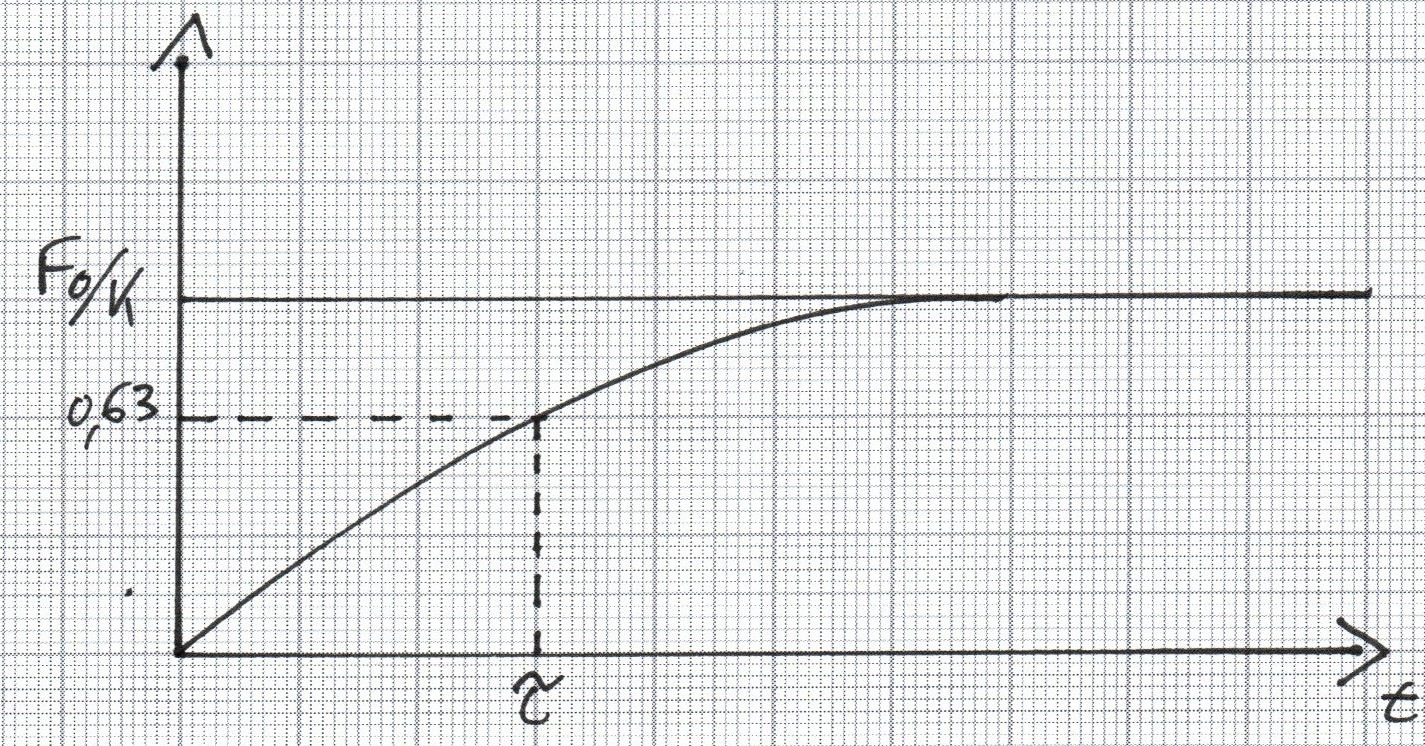
\includegraphics[width=0.4\linewidth]{fig/mm5}
	\label{fig:mm5}
\end{figure}	
	\[ y(\tau) = \dfrac{F_0}{k}\left[1- e^{-1}\right] = 0.63\dfrac{F_0}{k}  \]
	Al tempo $\tau$ raggiungo il $63\%$ del valore finale. 
	
	Solitamente si dà il tempo di $4\tau\div 5\tau$ per effettuare una misurazione in prima approssimazione più vicina al valore reale, passando il transitorio rimane la sola soluzione asintotica. 
	
	Logicamente per $\tau$ maggiori si hanno più sicurezze sul valore misurato, ma quanto è necessario aspettare? 	
	\[ y(3\tau) = 0.95\dfrac{F_0}{k} \hspace{1cm} y(3\tau) = 0.99\dfrac{F_0}{k}  \]	
	Anche in questo caso è possibile applicare il 
	\end{adjustwidth}
	%\newpage
	\subsubsection{Metodo delle sottotangenti per la determinazione del $\tau$} 	
	\begin{adjustwidth}{2in}{}
	\definecolor{ccqqqq}{rgb}{0.8,0.,0.}
	\definecolor{qqwuqq}{rgb}{0.,0.39215686274509803,0.}
	\begin{figure}[H]
		\centering
		\subfloat{\begin{tikzpicture}[line cap=round,line join=round,>=triangle 45]
				\begin{axis}[
					x=5cm,y=5cm,
					axis lines=middle,
					%					ymajorgrids=true,
					%					xmajorgrids=true,
					xmin=-0.18,
					xmax=1.85,
					ymin=0,
					ymax=1.45,
					ytick=\empty, xtick=\empty,
					xticklabels=\empty,yticklabels=\empty,extra x ticks={0,1}, extra y ticks={1},
					xlabel=$x$, ylabel=$y$]
					\clip(-0.2,-0.1) rectangle (1.8,1.4);
					%%%%%%%%%%%%%%%%%%%% ESPONENZIALE
					\draw[line width=2.pt,color=qqwuqq] (-0.009475320582989168,-0.009520353554631766) -- (-0.009475320582989168,-0.009520353554631766);
					\draw[line width=2.pt,color=qqwuqq] (-0.009475320582989168,-0.009520353554631766) -- (0.020419263291807807,0.020212201877181202);
					\draw[line width=2.pt,color=qqwuqq] (0.020419263291807807,0.020212201877181202) -- (0.05031384716660478,0.04906906931578725);
					\draw[line width=2.pt,color=qqwuqq] (0.05031384716660478,0.04906906931578725) -- (0.08020843104140175,0.07707603966446752);
					\draw[line width=2.pt,color=qqwuqq] (0.08020843104140175,0.07707603966446752) -- (0.11010301491619873,0.10425814422868185);
					\draw[line width=2.pt,color=qqwuqq] (0.11010301491619873,0.10425814422868185) -- (0.13999759879099571,0.13063967708786506);
					\draw[line width=2.pt,color=qqwuqq] (0.13999759879099571,0.13063967708786506) -- (0.1698921826657927,0.15624421680832656);
					\draw[line width=2.pt,color=qqwuqq] (0.1698921826657927,0.15624421680832656) -- (0.1997867665405897,0.18109464751665771);
					\draw[line width=2.pt,color=qqwuqq] (0.1997867665405897,0.18109464751665771) -- (0.22968135041538668,0.2052131793524813);
					\draw[line width=2.pt,color=qqwuqq] (0.22968135041538668,0.2052131793524813) -- (0.25957593429018366,0.22862136831882485);
					\draw[line width=2.pt,color=qqwuqq] (0.25957593429018366,0.22862136831882485) -- (0.28947051816498065,0.2513401355478557);
					\draw[line width=2.pt,color=qqwuqq] (0.28947051816498065,0.2513401355478557) -- (0.31936510203977764,0.27338978599919994);
					\draw[line width=2.pt,color=qqwuqq] (0.31936510203977764,0.27338978599919994) -- (0.3492596859145746,0.2947900266075545);
					\draw[line width=2.pt,color=qqwuqq] (0.3492596859145746,0.2947900266075545) -- (0.3791542697893716,0.31555998389581397);
					\draw[line width=2.pt,color=qqwuqq] (0.3791542697893716,0.31555998389581397) -- (0.4090488536641686,0.3357182210694515);
					\draw[line width=2.pt,color=qqwuqq] (0.4090488536641686,0.3357182210694515) -- (0.4389434375389656,0.3552827546074343);
					\draw[line width=2.pt,color=qqwuqq] (0.4389434375389656,0.3552827546074343) -- (0.4688380214137626,0.37427107036450036);
					\draw[line width=2.pt,color=qqwuqq] (0.4688380214137626,0.37427107036450036) -- (0.49873260528855956,0.392700139199188);
					\draw[line width=2.pt,color=qqwuqq] (0.49873260528855956,0.392700139199188) -- (0.5286271891633565,0.4105864321415871);
					\draw[line width=2.pt,color=qqwuqq] (0.5286271891633565,0.4105864321415871) -- (0.5585217730381534,0.4279459351143664);
					\draw[line width=2.pt,color=qqwuqq] (0.5585217730381534,0.4279459351143664) -- (0.5884163569129504,0.44479416322023546);
					\draw[line width=2.pt,color=qqwuqq] (0.5884163569129504,0.44479416322023546) -- (0.6183109407877473,0.4611461746086093);
					\draw[line width=2.pt,color=qqwuqq] (0.6183109407877473,0.4611461746086093) -- (0.6482055246625442,0.47701658393387003);
					\draw[line width=2.pt,color=qqwuqq] (0.6482055246625442,0.47701658393387003) -- (0.6781001085373412,0.49241957541725434);
					\draw[line width=2.pt,color=qqwuqq] (0.6781001085373412,0.49241957541725434) -- (0.7079946924121381,0.5073689155240391);
					\draw[line width=2.pt,color=qqwuqq] (0.7079946924121381,0.5073689155240391) -- (0.737889276286935,0.5218779652673565);
					\draw[line width=2.pt,color=qqwuqq] (0.737889276286935,0.5218779652673565) -- (0.767783860161732,0.535959692149637);
					\draw[line width=2.pt,color=qqwuqq] (0.767783860161732,0.535959692149637) -- (0.7976784440365289,0.5496266817523481);
					\draw[line width=2.pt,color=qqwuqq] (0.7976784440365289,0.5496266817523481) -- (0.8275730279113258,0.5628911489843931);
					\draw[line width=2.pt,color=qqwuqq] (0.8275730279113258,0.5628911489843931) -- (0.8574676117861227,0.5757649489992179);
					\draw[line width=2.pt,color=qqwuqq] (0.8574676117861227,0.5757649489992179) -- (0.8873621956609197,0.5882595877903873);
					\draw[line width=2.pt,color=qqwuqq] (0.8873621956609197,0.5882595877903873) -- (0.9172567795357166,0.6003862324750974);
					\draw[line width=2.pt,color=qqwuqq] (0.9172567795357166,0.6003862324750974) -- (0.9471513634105135,0.6121557212748165);
					\draw[line width=2.pt,color=qqwuqq] (0.9471513634105135,0.6121557212748165) -- (0.9770459472853105,0.6235785732019758);
					\draw[line width=2.pt,color=qqwuqq] (0.9770459472853105,0.6235785732019758) -- (1.0069405311601074,0.6346649974613642);
					\draw[line width=2.pt,color=qqwuqq] (1.0069405311601074,0.6346649974613642) -- (1.0368351150349044,0.645424902574633);
					\draw[line width=2.pt,color=qqwuqq] (1.0368351150349044,0.645424902574633) -- (1.0667296989097015,0.6558679052360645);
					\draw[line width=2.pt,color=qqwuqq] (1.0667296989097015,0.6558679052360645) -- (1.0966242827844985,0.6660033389075175);
					\draw[line width=2.pt,color=qqwuqq] (1.0966242827844985,0.6660033389075175) -- (1.1265188666592956,0.6758402621602345);
					\draw[line width=2.pt,color=qqwuqq] (1.1265188666592956,0.6758402621602345) -- (1.1564134505340926,0.6853874667709647);
					\draw[line width=2.pt,color=qqwuqq] (1.1564134505340926,0.6853874667709647) -- (1.1863080344088897,0.6946534855796378);
					\draw[line width=2.pt,color=qqwuqq] (1.1863080344088897,0.6946534855796378) -- (1.2162026182836867,0.7036466001156123);
					\draw[line width=2.pt,color=qqwuqq] (1.2162026182836867,0.7036466001156123) -- (1.2460972021584837,0.7123748479993158);
					\draw[line width=2.pt,color=qqwuqq] (1.2460972021584837,0.7123748479993158) -- (1.2759917860332808,0.7208460301258892);
					\draw[line width=2.pt,color=qqwuqq] (1.2759917860332808,0.7208460301258892) -- (1.3058863699080778,0.729067717637258);
					\draw[line width=2.pt,color=qqwuqq] (1.3058863699080778,0.729067717637258) -- (1.3357809537828749,0.7370472586888608);
					\draw[line width=2.pt,color=qqwuqq] (1.3357809537828749,0.7370472586888608) -- (1.365675537657672,0.7447917850170837);
					\draw[line width=2.pt,color=qqwuqq] (1.365675537657672,0.7447917850170837) -- (1.395570121532469,0.7523082183132678);
					\draw[line width=2.pt,color=qqwuqq] (1.395570121532469,0.7523082183132678) -- (1.425464705407266,0.7596032764099907);
					\draw[line width=2.pt,color=qqwuqq] (1.425464705407266,0.7596032764099907) -- (1.455359289282063,0.7666834792851469);
					\draw[line width=2.pt,color=qqwuqq] (1.455359289282063,0.7666834792851469) -- (1.48525387315686,0.7735551548891958);
					\draw[line width=2.pt,color=qqwuqq] (1.48525387315686,0.7735551548891958) -- (1.5151484570316571,0.7802244448007845);
					\draw[line width=2.pt,color=qqwuqq] (1.5151484570316571,0.7802244448007845) -- (1.5450430409064542,0.7866973097158003);
					\draw[line width=2.pt,color=qqwuqq] (1.5450430409064542,0.7866973097158003) -- (1.5749376247812512,0.792979534774759);
					\draw[line width=2.pt,color=qqwuqq] (1.5749376247812512,0.792979534774759) -- (1.6048322086560483,0.7990767347332898);
					\draw[line width=2.pt,color=qqwuqq] (1.6048322086560483,0.7990767347332898) -- (1.6347267925308453,0.8049943589803377);
					\draw[line width=2.pt,color=qqwuqq] (1.6347267925308453,0.8049943589803377) -- (1.6646213764056423,0.8107376964085707);
					\draw[line width=2.pt,color=qqwuqq] (1.6646213764056423,0.8107376964085707) -- (1.6945159602804394,0.8163118801413412);
					\draw[line width=2.pt,color=qqwuqq] (1.6945159602804394,0.8163118801413412) -- (1.7244105441552364,0.8217218921204285);
					\draw[line width=2.pt,color=qqwuqq] (1.7244105441552364,0.8217218921204285) -- (1.7543051280300335,0.826972567558664);
					\draw[line width=2.pt,color=qqwuqq] (1.7543051280300335,0.826972567558664) -- (1.7841997119048305,0.8320685992614145);
					\draw[line width=2.pt,color=qqwuqq] (1.7841997119048305,0.8320685992614145) -- (1.8140942957796276,0.8370145418207904);
					\draw[line width=2.pt,color=qqwuqq] (1.8140942957796276,0.8370145418207904) -- (1.8439888796544246,0.8418148156863242);
					\draw[line width=2.pt,color=qqwuqq] (1.8439888796544246,0.8418148156863242) -- (1.8738834635292216,0.8464737111157599);
					\draw[line width=2.pt,color=qqwuqq] (1.8738834635292216,0.8464737111157599) -- (1.9037780474040187,0.8509953920094816);
					\draw[line width=2.pt,color=qqwuqq] (1.9037780474040187,0.8509953920094816) -- (1.9336726312788157,0.8553838996320116);
					\draw[line width=2.pt,color=qqwuqq] (1.9336726312788157,0.8553838996320116) -- (1.9635672151536128,0.8596431562239008);
					\draw[line width=2.pt,color=qqwuqq] (1.9635672151536128,0.8596431562239008) -- (1.9934617990284098,0.8637769685072421);
					\draw[line width=2.pt,color=qqwuqq] (1.9934617990284098,0.8637769685072421) -- (2.0233563829032066,0.8677890310879386);
					\draw[line width=2.pt,color=qqwuqq] (2.0233563829032066,0.8677890310879386) -- (2.0532509667780037,0.8716829297577675);
					\draw[line width=2.pt,color=qqwuqq] (2.0532509667780037,0.8716829297577675) -- (2.0831455506528007,0.8754621446991911);
					\draw[line width=2.pt,color=qqwuqq] (2.0831455506528007,0.8754621446991911) -- (2.1130401345275978,0.8791300535957799);
					\draw[line width=2.pt,color=qqwuqq] (2.1130401345275978,0.8791300535957799) -- (2.142934718402395,0.8826899346510253);
					\draw[line width=2.pt,color=qqwuqq] (2.142934718402395,0.8826899346510253) -- (2.172829302277192,0.8861449695182437);
					\draw[line width=2.pt,color=qqwuqq] (2.172829302277192,0.8861449695182437) -- (2.202723886151989,0.8894982461441879);
					\draw[line width=2.pt,color=qqwuqq] (2.202723886151989,0.8894982461441879) -- (2.232618470026786,0.8927527615289069);
					\draw[line width=2.pt,color=qqwuqq] (2.232618470026786,0.8927527615289069) -- (2.262513053901583,0.8959114244043237);
					\draw[line width=2.pt,color=qqwuqq] (2.262513053901583,0.8959114244043237) -- (2.29240763777638,0.8989770578339219);
					\draw[line width=2.pt,color=qqwuqq] (2.29240763777638,0.8989770578339219) -- (2.322302221651177,0.9019524017358665);
					\draw[line width=2.pt,color=qqwuqq] (2.322302221651177,0.9019524017358665) -- (2.352196805525974,0.9048401153318131);
					\draw[line width=2.pt,color=qqwuqq] (2.352196805525974,0.9048401153318131) -- (2.382091389400771,0.9076427795235943);
					\draw[line width=2.pt,color=qqwuqq] (2.382091389400771,0.9076427795235943) -- (2.411985973275568,0.9103628991999078);
					\draw[line width=2.pt,color=qqwuqq] (2.411985973275568,0.9103628991999078) -- (2.4418805571503652,0.9130029054750676);
					\draw[line width=2.pt,color=qqwuqq] (2.4418805571503652,0.9130029054750676) -- (2.4717751410251623,0.9155651578618187);
					\draw[line width=2.pt,color=qqwuqq] (2.4717751410251623,0.9155651578618187) -- (2.5016697248999593,0.9180519463801584);
					\draw[line width=2.pt,color=qqwuqq] (2.5016697248999593,0.9180519463801584) -- (2.5315643087747564,0.9204654936040473);
					\draw[line width=2.pt,color=qqwuqq] (2.5315643087747564,0.9204654936040473) -- (2.5614588926495534,0.9228079566478412);
					\draw[line width=2.pt,color=qqwuqq] (2.5614588926495534,0.9228079566478412) -- (2.5913534765243504,0.925081429094218);
					\draw[line width=2.pt,color=qqwuqq] (2.5913534765243504,0.925081429094218) -- (2.6212480603991475,0.9272879428653223);
					\draw[line width=2.pt,color=qqwuqq] (2.6212480603991475,0.9272879428653223) -- (2.6511426442739445,0.9294294700388019);
					\draw[line width=2.pt,color=qqwuqq] (2.6511426442739445,0.9294294700388019) -- (2.6810372281487416,0.9315079246103573);
					\draw[line width=2.pt,color=qqwuqq] (2.6810372281487416,0.9315079246103573) -- (2.7109318120235386,0.9335251642043801);
					\draw[line width=2.pt,color=qqwuqq] (2.7109318120235386,0.9335251642043801) -- (2.7408263958983357,0.9354829917342111);
					\draw[line width=2.pt,color=qqwuqq] (2.7408263958983357,0.9354829917342111) -- (2.7707209797731327,0.9373831570134974);
					\draw[line width=2.pt,color=qqwuqq] (2.7707209797731327,0.9373831570134974) -- (2.8006155636479297,0.939227358320094);
					\draw[line width=2.pt,color=qqwuqq] (2.8006155636479297,0.939227358320094) -- (2.830510147522727,0.9410172439139041);
					\draw[line width=2.pt,color=qqwuqq] (2.830510147522727,0.9410172439139041) -- (2.860404731397524,0.9427544135100158);
					\draw[line width=2.pt,color=qqwuqq] (2.860404731397524,0.9427544135100158) -- (2.890299315272321,0.9444404197084514);
					\draw[line width=2.pt,color=qqwuqq] (2.890299315272321,0.9444404197084514) -- (2.920193899147118,0.9460767693818088);
					\draw[line width=2.pt,color=qqwuqq] (2.920193899147118,0.9460767693818088) -- (2.950088483021915,0.9476649250220319);
					\draw[line width=2.pt,color=qqwuqq] (2.950088483021915,0.9476649250220319) -- (2.979983066896712,0.9492063060475174);
					\draw[line width=2.pt,color=qqwuqq] (2.979983066896712,0.9492063060475174) -- (3.009877650771509,0.9507022900717236);
					\draw[line width=2.pt,color=qqwuqq] (3.009877650771509,0.9507022900717236) -- (3.039772234646306,0.9521542141344163);
					\draw[line width=2.pt,color=qqwuqq] (3.039772234646306,0.9521542141344163) -- (3.069666818521103,0.9535633758966512);
					\draw[line width=2.pt,color=qqwuqq] (3.069666818521103,0.9535633758966512) -- (3.0995614023959,0.954931034800563);
					\draw[line width=2.pt,color=qqwuqq] (3.0995614023959,0.954931034800563) -- (3.129455986270697,0.9562584131949938);
					\draw[line width=2.pt,color=qqwuqq] (3.129455986270697,0.9562584131949938) -- (3.1593505701454943,0.9575466974279724);
					\draw[line width=2.pt,color=qqwuqq] (3.1593505701454943,0.9575466974279724) -- (3.1892451540202913,0.9587970389070142);
					\draw[line width=2.pt,color=qqwuqq] (3.1892451540202913,0.9587970389070142) -- (3.2191397378950883,0.9600105551281963);
					\draw[line width=2.pt,color=qqwuqq] (3.2191397378950883,0.9600105551281963) -- (3.2490343217698854,0.9611883306749218);
					\draw[line width=2.pt,color=qqwuqq] (3.2490343217698854,0.9611883306749218) -- (3.2789289056446824,0.9623314181872695);
					\draw[line width=2.pt,color=qqwuqq] (3.2789289056446824,0.9623314181872695) -- (3.3088234895194795,0.9634408393027936);
					\draw[line width=2.pt,color=qqwuqq] (3.3088234895194795,0.9634408393027936) -- (3.3387180733942765,0.964517585569615);
					\draw[line width=2.pt,color=qqwuqq] (3.3387180733942765,0.964517585569615) -- (3.3686126572690736,0.9655626193326207);
					\draw[line width=2.pt,color=qqwuqq] (3.3686126572690736,0.9655626193326207) -- (3.3985072411438706,0.9665768745935611);
					\draw[line width=2.pt,color=qqwuqq] (3.3985072411438706,0.9665768745935611) -- (3.4284018250186676,0.9675612578458178);
					\draw[line width=2.pt,color=qqwuqq] (3.4284018250186676,0.9675612578458178) -- (3.4582964088934647,0.9685166488845833);
					\draw[line width=2.pt,color=qqwuqq] (3.4582964088934647,0.9685166488845833) -- (3.4881909927682617,0.9694439015931814);
					\draw[line width=2.pt,color=qqwuqq] (3.4881909927682617,0.9694439015931814) -- (3.5180855766430588,0.9703438447062268);
					\draw[line width=2.pt,color=qqwuqq] (3.5180855766430588,0.9703438447062268) -- (3.547980160517856,0.9712172825503097);
					\draw[line width=2.pt,color=qqwuqq] (3.547980160517856,0.9712172825503097) -- (3.577874744392653,0.9720649957628643);
					\draw[line width=2.pt,color=qqwuqq] (3.577874744392653,0.9720649957628643) -- (3.60776932826745,0.9728877419898662);
					\draw[line width=2.pt,color=qqwuqq] (3.60776932826745,0.9728877419898662) -- (3.637663912142247,0.9736862565629795);
					\draw[line width=2.pt,color=qqwuqq] (3.637663912142247,0.9736862565629795) -- (3.667558496017044,0.9744612531567628);
					\draw[line width=2.pt,color=qqwuqq] (3.667558496017044,0.9744612531567628) -- (3.697453079891841,0.9752134244265166);
					\draw[line width=2.pt,color=qqwuqq] (3.697453079891841,0.9752134244265166) -- (3.727347663766638,0.9759434426273469);
					\draw[line width=2.pt,color=qqwuqq] (3.727347663766638,0.9759434426273469) -- (3.757242247641435,0.9766519602149938);
					\draw[line width=2.pt,color=qqwuqq] (3.757242247641435,0.9766519602149938) -- (3.787136831516232,0.9773396104289667);
					\draw[line width=2.pt,color=qqwuqq] (3.787136831516232,0.9773396104289667) -- (3.817031415391029,0.9780070078585033);
					\draw[line width=2.pt,color=qqwuqq] (3.817031415391029,0.9780070078585033) -- (3.8469259992658262,0.9786547489918603);
					\draw[line width=2.pt,color=qqwuqq] (3.8469259992658262,0.9786547489918603) -- (3.8768205831406233,0.9792834127494268);
					\draw[line width=2.pt,color=qqwuqq] (3.8768205831406233,0.9792834127494268) -- (3.9067151670154203,0.9798935610011354);
					\draw[line width=2.pt,color=qqwuqq] (3.9067151670154203,0.9798935610011354) -- (3.9366097508902174,0.9804857390686357);
					\draw[line width=2.pt,color=qqwuqq] (3.9366097508902174,0.9804857390686357) -- (3.9665043347650144,0.9810604762126761);
					\draw[line width=2.pt,color=qqwuqq] (3.9665043347650144,0.9810604762126761) -- (3.9963989186398114,0.9816182861061329);
					\draw[line width=2.pt,color=qqwuqq] (3.9963989186398114,0.9816182861061329) -- (4.0262935025146085,0.9821596672931061);
					\draw[line width=2.pt,color=qqwuqq] (4.0262935025146085,0.9821596672931061) -- (4.0561880863894055,0.9826851036344953);
					\draw[line width=2.pt,color=qqwuqq] (4.0561880863894055,0.9826851036344953) -- (4.086082670264203,0.983195064740451);
					\draw[line width=2.pt,color=qqwuqq] (4.086082670264203,0.983195064740451) -- (4.115977254139,0.9836900063900902);
					\draw[line width=2.pt,color=qqwuqq] (4.115977254139,0.9836900063900902) -- (4.145871838013797,0.98417037093885);
					\draw[line width=2.pt,color=qqwuqq] (4.145871838013797,0.98417037093885) -- (4.175766421888594,0.9846365877138447);
					\draw[line width=2.pt,color=qqwuqq] (4.175766421888594,0.9846365877138447) -- (4.205661005763391,0.985089073397577);
					\draw[line width=2.pt,color=qqwuqq] (4.205661005763391,0.985089073397577) -- (4.235555589638188,0.9855282324003501);
					\draw[line width=2.pt,color=qqwuqq] (4.235555589638188,0.9855282324003501) -- (4.265450173512985,0.9859544572217099);
					\draw[line width=2.pt,color=qqwuqq] (4.265450173512985,0.9859544572217099) -- (4.295344757387782,0.9863681288012427);
					\draw[line width=2.pt,color=qqwuqq] (4.295344757387782,0.9863681288012427) -- (4.325239341262579,0.9867696168590409);
					\draw[line width=2.pt,color=qqwuqq] (4.325239341262579,0.9867696168590409) -- (4.355133925137376,0.9871592802261415);
					\draw[line width=2.pt,color=qqwuqq] (4.355133925137376,0.9871592802261415) -- (4.385028509012173,0.9875374671652323);
					\draw[line width=2.pt,color=qqwuqq] (4.385028509012173,0.9875374671652323) -- (4.41492309288697,0.9879045156819123);
					\draw[line width=2.pt,color=qqwuqq] (4.41492309288697,0.9879045156819123) -- (4.444817676761767,0.9882607538267856);
					\draw[line width=2.pt,color=qqwuqq] (4.444817676761767,0.9882607538267856) -- (4.474712260636564,0.9886064999886572);
					\draw[line width=2.pt,color=qqwuqq] (4.474712260636564,0.9886064999886572) -- (4.504606844511361,0.9889420631790939);
					\draw[line width=2.pt,color=qqwuqq] (4.504606844511361,0.9889420631790939) -- (4.534501428386158,0.9892677433086043);
					\draw[line width=2.pt,color=qqwuqq] (4.534501428386158,0.9892677433086043) -- (4.564396012260955,0.9895838314546846);
					\draw[line width=2.pt,color=qqwuqq] (4.564396012260955,0.9895838314546846) -- (4.594290596135752,0.9898906101219698);
					\draw[line width=2.pt,color=qqwuqq] (4.594290596135752,0.9898906101219698) -- (4.624185180010549,0.9901883534947229);
					\draw[line width=2.pt,color=qqwuqq] (4.624185180010549,0.9901883534947229) -- (4.654079763885346,0.9904773276818885);
					\draw[line width=2.pt,color=qqwuqq] (4.654079763885346,0.9904773276818885) -- (4.683974347760143,0.9907577909549272);
					\draw[line width=2.pt,color=qqwuqq] (4.683974347760143,0.9907577909549272) -- (4.7138689316349405,0.9910299939786479);
					\draw[line width=2.pt,color=qqwuqq] (4.7138689316349405,0.9910299939786479) -- (4.7437635155097375,0.9912941800352384);
					\draw[line width=2.pt,color=qqwuqq] (4.7437635155097375,0.9912941800352384) -- (4.773658099384535,0.9915505852417014);
					\draw[line width=2.pt,color=qqwuqq] (4.773658099384535,0.9915505852417014) -- (4.803552683259332,0.991799438760883);
					\draw[line width=2.pt,color=qqwuqq] (4.803552683259332,0.991799438760883) -- (4.833447267134129,0.9920409630062886);
					\draw[line width=2.pt,color=qqwuqq] (4.833447267134129,0.9920409630062886) -- (4.863341851008926,0.9922753738408658);
					\draw[line width=2.pt,color=qqwuqq] (4.863341851008926,0.9922753738408658) -- (4.893236434883723,0.9925028807699314);
					\draw[line width=2.pt,color=qqwuqq] (4.893236434883723,0.9925028807699314) -- (4.92313101875852,0.9927236871284185);
					\draw[line width=2.pt,color=qqwuqq] (4.92313101875852,0.9927236871284185) -- (4.953025602633317,0.9929379902626067);
					\draw[line width=2.pt,color=qqwuqq] (4.953025602633317,0.9929379902626067) -- (4.982920186508114,0.9931459817065015);
					\draw[line width=2.pt,color=qqwuqq] (4.982920186508114,0.9931459817065015) -- (5.012814770382911,0.9933478473530182);
					\draw[line width=2.pt,color=qqwuqq] (5.012814770382911,0.9933478473530182) -- (5.042709354257708,0.9935437676201241);
					\draw[line width=2.pt,color=qqwuqq] (5.042709354257708,0.9935437676201241) -- (5.072603938132505,0.9937339176120875);
					\draw[line width=2.pt,color=qqwuqq] (5.072603938132505,0.9937339176120875) -- (5.102498522007302,0.9939184672759779);
					\draw[line width=2.pt,color=qqwuqq] (5.102498522007302,0.9939184672759779) -- (5.132393105882099,0.994097581553556);
					\draw[line width=2.pt,color=qqwuqq] (5.132393105882099,0.994097581553556) -- (5.162287689756896,0.9942714205286918);
					\draw[line width=2.pt,color=qqwuqq] (5.162287689756896,0.9942714205286918) -- (5.192182273631693,0.9944401395704392);
					\draw[line width=2.pt,color=qqwuqq] (5.192182273631693,0.9944401395704392) -- (5.22207685750649,0.9946038894718978);
					\draw[line width=2.pt,color=qqwuqq] (5.22207685750649,0.9946038894718978) -- (5.251971441381287,0.9947628165849848);
					\draw[line width=2.pt,color=qqwuqq] (5.251971441381287,0.9947628165849848) -- (5.281866025256084,0.994917062951237);
					\draw[line width=2.pt,color=qqwuqq] (5.281866025256084,0.994917062951237) -- (5.311760609130881,0.9950667664287615);
					\draw[line width=2.pt,color=qqwuqq] (5.311760609130881,0.9950667664287615) -- (5.341655193005678,0.9952120608154457);
					\draw[line width=2.pt,color=qqwuqq] (5.341655193005678,0.9952120608154457) -- (5.371549776880475,0.9953530759685405);
					\draw[line width=2.pt,color=qqwuqq] (5.371549776880475,0.9953530759685405) -- (5.4014443607552725,0.9954899379207204);
					\draw[line width=2.pt,color=qqwuqq] (5.4014443607552725,0.9954899379207204) -- (5.4313389446300695,0.995622768992725);
					\draw[line width=2.pt,color=qqwuqq] (5.4313389446300695,0.995622768992725) -- (5.4612335285048665,0.9957516879026839);
					\draw[line width=2.pt,color=qqwuqq] (5.4612335285048665,0.9957516879026839) -- (5.491128112379664,0.9958768098722216);
					\draw[line width=2.pt,color=qqwuqq] (5.491128112379664,0.9958768098722216) -- (5.521022696254461,0.9959982467294364);
					\draw[line width=2.pt,color=qqwuqq] (5.521022696254461,0.9959982467294364) -- (5.550917280129258,0.9961161070088478);
					\draw[line width=2.pt,color=qqwuqq] (5.550917280129258,0.9961161070088478) -- (5.580811864004055,0.9962304960483992);
					\draw[line width=2.pt,color=qqwuqq] (5.580811864004055,0.9962304960483992) -- (5.610706447878852,0.9963415160836038);
					\draw[line width=2.pt,color=qqwuqq] (5.610706447878852,0.9963415160836038) -- (5.640601031753649,0.9964492663389183);
					\draw[line width=2.pt,color=qqwuqq] (5.640601031753649,0.9964492663389183) -- (5.670495615628446,0.9965538431164245);
					\draw[line width=2.pt,color=qqwuqq] (5.670495615628446,0.9965538431164245) -- (5.700390199503243,0.9966553398819001);
					\draw[line width=2.pt,color=qqwuqq] (5.700390199503243,0.9966553398819001) -- (5.73028478337804,0.9967538473483537);
					\draw[line width=2.pt,color=qqwuqq] (5.73028478337804,0.9967538473483537) -- (5.760179367252837,0.9968494535570996);
					\draw[line width=2.pt,color=qqwuqq] (5.760179367252837,0.9968494535570996) -- (5.790073951127634,0.9969422439564455);
					\draw[line width=2.pt,color=qqwuqq] (5.790073951127634,0.9969422439564455) -- (5.819968535002431,0.9970323014780613);
					\draw[line width=2.pt,color=qqwuqq] (5.819968535002431,0.9970323014780613) -- (5.849863118877228,0.9971197066111007);
					\draw[line width=2.pt,color=qqwuqq] (5.849863118877228,0.9971197066111007) -- (5.879757702752025,0.9972045374741376);
					\draw[line width=2.pt,color=qqwuqq] (5.879757702752025,0.9972045374741376) -- (5.909652286626822,0.9972868698849852);
					\draw[line width=2.pt,color=qqwuqq] (5.909652286626822,0.9972868698849852) -- (5.939546870501619,0.997366777428458);
					\draw[line width=2.pt,color=qqwuqq] (5.939546870501619,0.997366777428458) -- (5.969441454376416,0.9974443315221392);
					\draw[line width=2.pt,color=qqwuqq] (5.969441454376416,0.9974443315221392) -- (5.999336038251213,0.9975196014802097);
					\draw[line width=2.pt,color=qqwuqq] (5.999336038251213,0.9975196014802097) -- (6.02923062212601,0.9975926545753979);
					\draw[line width=2.pt,color=qqwuqq] (6.02923062212601,0.9975926545753979) -- (6.059125206000807,0.9976635560991051);
					\draw[line width=2.pt,color=qqwuqq] (6.059125206000807,0.9976635560991051) -- (6.089019789875604,0.9977323694197598);
					\draw[line width=2.pt,color=qqwuqq] (6.089019789875604,0.9977323694197598) -- (6.1189143737504015,0.9977991560394536);
					\draw[line width=2.pt,color=qqwuqq] (6.1189143737504015,0.9977991560394536) -- (6.1488089576251985,0.9978639756489079);
					\draw[line width=2.pt,color=qqwuqq] (6.1488089576251985,0.9978639756489079) -- (6.178703541499996,0.9979268861808244);
					\draw[line width=2.pt,color=qqwuqq] (6.178703541499996,0.9979268861808244) -- (6.208598125374793,0.9979879438616607);
					\draw[line width=2.pt,color=qqwuqq] (6.208598125374793,0.9979879438616607) -- (6.23849270924959,0.9980472032618842);
					\draw[line width=2.pt,color=qqwuqq] (6.23849270924959,0.9980472032618842) -- (6.268387293124387,0.9981047173447442);
					\draw[line width=2.pt,color=qqwuqq] (6.268387293124387,0.9981047173447442) -- (6.298281876999184,0.9981605375136074);
					\draw[line width=2.pt,color=qqwuqq] (6.298281876999184,0.9981605375136074) -- (6.328176460873981,0.9982147136579009);
					\draw[line width=2.pt,color=qqwuqq] (6.328176460873981,0.9982147136579009) -- (6.358071044748778,0.9982672941977001);
					\draw[line width=2.pt,color=qqwuqq] (6.358071044748778,0.9982672941977001) -- (6.387965628623575,0.9983183261270044);
					\draw[line width=2.pt,color=qqwuqq] (6.387965628623575,0.9983183261270044) -- (6.417860212498372,0.9983678550557388);
					\draw[line width=2.pt,color=qqwuqq] (6.417860212498372,0.9983678550557388) -- (6.447754796373169,0.998415925250517);
					\draw[line width=2.pt,color=qqwuqq] (6.447754796373169,0.998415925250517) -- (6.477649380247966,0.9984625796742057);
					\draw[line width=2.pt,color=qqwuqq] (6.477649380247966,0.9984625796742057) -- (6.507543964122763,0.9985078600243222);
					\draw[line width=2.pt,color=qqwuqq] (6.507543964122763,0.9985078600243222) -- (6.53743854799756,0.9985518067703018);
					\draw[line width=2.pt,color=qqwuqq] (6.53743854799756,0.9985518067703018) -- (6.567333131872357,0.9985944591896675);
					\draw[line width=2.pt,color=qqwuqq] (6.567333131872357,0.9985944591896675) -- (6.597227715747154,0.9986358554031344);
					\draw[line width=2.pt,color=qqwuqq] (6.597227715747154,0.9986358554031344) -- (6.627122299621951,0.9986760324086801);
					\draw[line width=2.pt,color=qqwuqq] (6.627122299621951,0.9986760324086801) -- (6.657016883496748,0.998715026114612);
					\draw[line width=2.pt,color=qqwuqq] (6.657016883496748,0.998715026114612) -- (6.686911467371545,0.9987528713716604);
					\draw[line width=2.pt,color=qqwuqq] (6.686911467371545,0.9987528713716604) -- (6.716806051246342,0.9987896020041257);
					\draw[line width=2.pt,color=qqwuqq] (6.716806051246342,0.9987896020041257) -- (6.746700635121139,0.9988252508401102);
					\draw[line width=2.pt,color=qqwuqq] (6.746700635121139,0.9988252508401102) -- (6.776595218995936,0.9988598497408574);
					\draw[line width=2.pt,color=qqwuqq] (6.776595218995936,0.9988598497408574) -- (6.8064898028707335,0.9988934296292283);
					\draw[line width=2.pt,color=qqwuqq] (6.8064898028707335,0.9988934296292283) -- (6.8363843867455305,0.998926020517339);
					\draw[line width=2.pt,color=qqwuqq] (6.8363843867455305,0.998926020517339) -- (6.8662789706203275,0.9989576515333838);
					\draw[line width=2.pt,color=qqwuqq] (6.8662789706203275,0.9989576515333838) -- (6.896173554495125,0.9989883509476688);
					\draw[line width=2.pt,color=qqwuqq] (6.896173554495125,0.9989883509476688) -- (6.926068138369922,0.9990181461978785);
					\draw[line width=2.pt,color=qqwuqq] (6.926068138369922,0.9990181461978785) -- (6.955962722244719,0.9990470639135984);
					\draw[line width=2.pt,color=qqwuqq] (6.955962722244719,0.9990470639135984) -- (6.985857306119516,0.999075129940115);
					\draw[line width=2.pt,color=qqwuqq] (6.985857306119516,0.999075129940115) -- (7.015751889994313,0.9991023693615154);
					\draw[line width=2.pt,color=qqwuqq] (7.015751889994313,0.9991023693615154) -- (7.04564647386911,0.9991288065231061);
					\draw[line width=2.pt,color=qqwuqq] (7.04564647386911,0.9991288065231061) -- (7.075541057743907,0.9991544650531717);
					\draw[line width=2.pt,color=qqwuqq] (7.075541057743907,0.9991544650531717) -- (7.105435641618704,0.999179367884093);
					\draw[line width=2.pt,color=qqwuqq] (7.105435641618704,0.999179367884093) -- (7.135330225493501,0.9992035372728423);
					\draw[line width=2.pt,color=qqwuqq] (7.135330225493501,0.9992035372728423) -- (7.165224809368298,0.9992269948208761);
					\draw[line width=2.pt,color=qqwuqq] (7.165224809368298,0.9992269948208761) -- (7.195119393243095,0.9992497614934414);
					\draw[line width=2.pt,color=qqwuqq] (7.195119393243095,0.9992497614934414) -- (7.225013977117892,0.9992718576383133);
					\draw[line width=2.pt,color=qqwuqq] (7.225013977117892,0.9992718576383133) -- (7.254908560992689,0.9992933030039811);
					\draw[line width=2.pt,color=qqwuqq] (7.254908560992689,0.9992933030039811) -- (7.284803144867486,0.9993141167572984);
					\draw[line width=2.pt,color=qqwuqq] (7.284803144867486,0.9993141167572984) -- (7.314697728742283,0.9993343175006133);
					\draw[line width=2.pt,color=qqwuqq] (7.314697728742283,0.9993343175006133) -- (7.34459231261708,0.9993539232883949);
					\draw[line width=2.pt,color=qqwuqq] (7.34459231261708,0.9993539232883949) -- (7.374486896491877,0.999372951643369);
					\draw[line width=2.pt,color=qqwuqq] (7.374486896491877,0.999372951643369) -- (7.404381480366674,0.9993914195721793);
					\draw[line width=2.pt,color=qqwuqq] (7.404381480366674,0.9993914195721793) -- (7.434276064241471,0.999409343580587);
					\draw[line width=2.pt,color=qqwuqq] (7.434276064241471,0.999409343580587) -- (7.464170648116268,0.9994267396882232);
					\draw[line width=2.pt,color=qqwuqq] (7.464170648116268,0.9994267396882232) -- (7.4940652319910654,0.999443623442906);
					\draw[line width=2.pt,color=qqwuqq] (7.4940652319910654,0.999443623442906) -- (7.5239598158658625,0.999460009934537);
					\draw[line width=2.pt,color=qqwuqq] (7.5239598158658625,0.999460009934537) -- (7.5538543997406595,0.9994759138085871);
					\draw[line width=2.pt,color=qqwuqq] (7.5538543997406595,0.9994759138085871) -- (7.583748983615457,0.9994913492791869);
					\draw[line width=2.pt,color=qqwuqq] (7.583748983615457,0.9994913492791869) -- (7.613643567490254,0.9995063301418301);
					\draw[line width=2.pt,color=qqwuqq] (7.613643567490254,0.9995063301418301) -- (7.643538151365051,0.9995208697857029);
					\draw[line width=2.pt,color=qqwuqq] (7.643538151365051,0.9995208697857029) -- (7.673432735239848,0.9995349812056514);
					\draw[line width=2.pt,color=qqwuqq] (7.673432735239848,0.9995349812056514) -- (7.703327319114645,0.9995486770137955);
					\draw[line width=2.pt,color=qqwuqq] (7.703327319114645,0.9995486770137955) -- (7.733221902989442,0.9995619694508006);
					\draw[line width=2.pt,color=qqwuqq] (7.733221902989442,0.9995619694508006) -- (7.763116486864239,0.9995748703968182);
					\draw[line width=2.pt,color=qqwuqq] (7.763116486864239,0.9995748703968182) -- (7.793011070739036,0.9995873913821037);
					\draw[line width=2.pt,color=qqwuqq] (7.793011070739036,0.9995873913821037) -- (7.822905654613833,0.9995995435973216);
					\draw[line width=2.pt,color=qqwuqq] (7.822905654613833,0.9995995435973216) -- (7.85280023848863,0.9996113379035471);
					\draw[line width=2.pt,color=qqwuqq] (7.85280023848863,0.9996113379035471) -- (7.882694822363427,0.9996227848419732);
					\draw[line width=2.pt,color=qqwuqq] (7.882694822363427,0.9996227848419732) -- (7.912589406238224,0.9996338946433321);
					\draw[line width=2.pt,color=qqwuqq] (7.912589406238224,0.9996338946433321) -- (7.942483990113021,0.9996446772370388);
					\draw[line width=2.pt,color=qqwuqq] (7.942483990113021,0.9996446772370388) -- (7.972378573987818,0.9996551422600656);
					\draw[line width=2.pt,color=qqwuqq] (7.972378573987818,0.9996551422600656) -- (8.002273157862614,0.999665299065555);
					\draw[line width=2.pt,color=qqwuqq] (8.002273157862614,0.999665299065555) -- (8.03216774173741,0.9996751567311795);
					\draw[line width=2.pt,color=qqwuqq] (8.03216774173741,0.9996751567311795) -- (8.062062325612207,0.9996847240672544);
					\draw[line width=2.pt,color=qqwuqq] (8.062062325612207,0.9996847240672544) -- (8.091956909487003,0.999694009624612);
					\draw[line width=2.pt,color=qqwuqq] (8.091956909487003,0.999694009624612) -- (8.121851493361799,0.9997030217022446);
					\draw[line width=2.pt,color=qqwuqq] (8.121851493361799,0.9997030217022446) -- (8.151746077236595,0.9997117683547206);
					\draw[line width=2.pt,color=qqwuqq] (8.151746077236595,0.9997117683547206) -- (8.181640661111391,0.9997202573993845);
					\draw[line width=2.pt,color=qqwuqq] (8.181640661111391,0.9997202573993845) -- (8.211535244986187,0.9997284964233429);
					\draw[line width=2.pt,color=qqwuqq] (8.211535244986187,0.9997284964233429) -- (8.241429828860984,0.9997364927902458);
					\draw[line width=2.pt,color=qqwuqq] (8.241429828860984,0.9997364927902458) -- (8.27132441273578,0.9997442536468675);
					\draw[line width=2.pt,color=qqwuqq] (8.27132441273578,0.9997442536468675) -- (8.301218996610576,0.9997517859294949);
					\draw[line width=2.pt,color=qqwuqq] (8.301218996610576,0.9997517859294949) -- (8.331113580485372,0.9997590963701256);
					\draw[line width=2.pt,color=qqwuqq] (8.331113580485372,0.9997590963701256) -- (8.361008164360168,0.999766191502486);
					\draw[line width=2.pt,color=qqwuqq] (8.361008164360168,0.999766191502486) -- (8.390902748234964,0.9997730776678697);
					\draw[line width=2.pt,color=qqwuqq] (8.390902748234964,0.9997730776678697) -- (8.42079733210976,0.9997797610208056);
					\draw[line width=2.pt,color=qqwuqq] (8.42079733210976,0.9997797610208056) -- (8.450691915984557,0.9997862475345585);
					\draw[line width=2.pt,color=qqwuqq] (8.450691915984557,0.9997862475345585) -- (8.480586499859353,0.9997925430064676);
					\draw[line width=2.pt,color=qqwuqq] (8.480586499859353,0.9997925430064676) -- (8.510481083734149,0.9997986530631278);
					\draw[line width=2.pt,color=qqwuqq] (8.510481083734149,0.9997986530631278) -- (8.540375667608945,0.999804583165419);
					\draw[line width=2.pt,color=qqwuqq] (8.540375667608945,0.999804583165419) -- (8.570270251483741,0.999810338613386);
					\draw[line width=2.pt,color=qqwuqq] (8.570270251483741,0.999810338613386) -- (8.600164835358537,0.9998159245509759);
					\draw[line width=2.pt,color=qqwuqq] (8.600164835358537,0.9998159245509759) -- (8.630059419233334,0.9998213459706358);
					\draw[line width=2.pt,color=qqwuqq] (8.630059419233334,0.9998213459706358) -- (8.65995400310813,0.9998266077177739);
					\draw[line width=2.pt,color=qqwuqq] (8.65995400310813,0.9998266077177739) -- (8.689848586982926,0.999831714495091);
					\draw[line width=2.pt,color=qqwuqq] (8.689848586982926,0.999831714495091) -- (8.719743170857722,0.9998366708667832);
					\draw[line width=2.pt,color=qqwuqq] (8.719743170857722,0.9998366708667832) -- (8.749637754732518,0.9998414812626211);
					\draw[line width=2.pt,color=qqwuqq] (8.749637754732518,0.9998414812626211) -- (8.779532338607314,0.9998461499819089);
					\draw[line width=2.pt,color=qqwuqq] (8.779532338607314,0.9998461499819089) -- (8.80942692248211,0.9998506811973272);
					\draw[line width=2.pt,color=qqwuqq] (8.80942692248211,0.9998506811973272) -- (8.839321506356907,0.9998550789586619);
					\draw[line width=2.pt,color=qqwuqq] (8.839321506356907,0.9998550789586619) -- (8.869216090231703,0.9998593471964242);
					\draw[line width=2.pt,color=qqwuqq] (8.869216090231703,0.9998593471964242) -- (8.899110674106499,0.9998634897253631);
					\draw[line width=2.pt,color=qqwuqq] (8.899110674106499,0.9998634897253631) -- (8.929005257981295,0.9998675102478749);
					\draw[line width=2.pt,color=qqwuqq] (8.929005257981295,0.9998675102478749) -- (8.958899841856091,0.9998714123573127);
					\draw[line width=2.pt,color=qqwuqq] (8.958899841856091,0.9998714123573127) -- (8.988794425730887,0.9998751995411972);
					\draw[line width=2.pt,color=qqwuqq] (8.988794425730887,0.9998751995411972) -- (9.018689009605684,0.9998788751843343);
					\draw[line width=2.pt,color=qqwuqq] (9.018689009605684,0.9998788751843343) -- (9.04858359348048,0.9998824425718399);
					\draw[line width=2.pt,color=qqwuqq] (9.04858359348048,0.9998824425718399) -- (9.078478177355276,0.9998859048920763);
					\draw[line width=2.pt,color=qqwuqq] (9.078478177355276,0.9998859048920763) -- (9.108372761230072,0.9998892652395016);
					\draw[line width=2.pt,color=qqwuqq] (9.108372761230072,0.9998892652395016) -- (9.138267345104868,0.9998925266174353);
					\draw[line width=2.pt,color=qqwuqq] (9.138267345104868,0.9998925266174353) -- (9.168161928979664,0.9998956919407429);
					\draw[line width=2.pt,color=qqwuqq] (9.168161928979664,0.9998956919407429) -- (9.19805651285446,0.9998987640384405);
					\draw[line width=2.pt,color=qqwuqq] (9.19805651285446,0.9998987640384405) -- (9.227951096729257,0.9999017456562238);
					\draw[line width=2.pt,color=qqwuqq] (9.227951096729257,0.9999017456562238) -- (9.257845680604053,0.9999046394589217);
					\draw[line width=2.pt,color=qqwuqq] (9.257845680604053,0.9999046394589217) -- (9.287740264478849,0.9999074480328782);
					\draw[line width=2.pt,color=qqwuqq] (9.287740264478849,0.9999074480328782) -- (9.317634848353645,0.9999101738882641);
					\draw[line width=2.pt,color=qqwuqq] (9.317634848353645,0.9999101738882641) -- (9.347529432228441,0.9999128194613196);
					\draw[line width=2.pt,color=qqwuqq] (9.347529432228441,0.9999128194613196) -- (9.377424016103237,0.999915387116533);
					\draw[line width=2.pt,color=qqwuqq] (9.377424016103237,0.999915387116533) -- (9.407318599978034,0.9999178791487532);
					\draw[line width=2.pt,color=qqwuqq] (9.407318599978034,0.9999178791487532) -- (9.43721318385283,0.9999202977852405);
					\draw[line width=2.pt,color=qqwuqq] (9.43721318385283,0.9999202977852405) -- (9.467107767727626,0.9999226451876579);
					\draw[line width=2.pt,color=qqwuqq] (9.467107767727626,0.9999226451876579) -- (9.497002351602422,0.9999249234540027);
					\draw[line width=2.pt,color=qqwuqq] (9.497002351602422,0.9999249234540027) -- (9.526896935477218,0.9999271346204816);
					\draw[line width=2.pt,color=qqwuqq] (9.526896935477218,0.9999271346204816) -- (9.556791519352014,0.9999292806633305);
					\draw[line width=2.pt,color=qqwuqq] (9.556791519352014,0.9999292806633305) -- (9.58668610322681,0.9999313635005811);
					\draw[line width=2.pt,color=qqwuqq] (9.58668610322681,0.9999313635005811) -- (9.616580687101607,0.9999333849937748);
					\draw[line width=2.pt,color=qqwuqq] (9.616580687101607,0.9999333849937748) -- (9.646475270976403,0.9999353469496266);
					\draw[line width=2.pt,color=qqwuqq] (9.646475270976403,0.9999353469496266) -- (9.676369854851199,0.9999372511216399);
					\draw[line width=2.pt,color=qqwuqq] (9.676369854851199,0.9999372511216399) -- (9.706264438725995,0.9999390992116735);
					\draw[line width=2.pt,color=qqwuqq] (9.706264438725995,0.9999390992116735) -- (9.736159022600791,0.9999408928714629);
					\draw[line width=2.pt,color=qqwuqq] (9.736159022600791,0.9999408928714629) -- (9.766053606475587,0.9999426337040964);
					\draw[line width=2.pt,color=qqwuqq] (9.766053606475587,0.9999426337040964) -- (9.795948190350384,0.9999443232654478);
					\draw[line width=2.pt,color=qqwuqq] (9.795948190350384,0.9999443232654478) -- (9.82584277422518,0.9999459630655673);
					\draw[line width=2.pt,color=qqwuqq] (9.82584277422518,0.9999459630655673) -- (9.855737358099976,0.9999475545700305);
					\draw[line width=2.pt,color=qqwuqq] (9.855737358099976,0.9999475545700305) -- (9.885631941974772,0.9999490992012489);
					\draw[line width=2.pt,color=qqwuqq] (9.885631941974772,0.9999490992012489) -- (9.915526525849568,0.9999505983397408);
					\draw[line width=2.pt,color=qqwuqq] (9.915526525849568,0.9999505983397408) -- (9.945421109724364,0.9999520533253653);
					\draw[line width=2.pt,color=qqwuqq] (9.945421109724364,0.9999520533253653) -- (9.97531569359916,0.9999534654585198);
					\draw[line width=2.pt,color=qqwuqq] (9.97531569359916,0.9999534654585198) -- (10.005210277473957,0.999954836001302);
					\draw[line width=2.pt,color=qqwuqq] (10.005210277473957,0.999954836001302) -- (10.035104861348753,0.9999561661786383);
					\draw[line width=2.pt,color=qqwuqq] (10.035104861348753,0.9999561661786383) -- (10.064999445223549,0.9999574571793782);
					\draw[line width=2.pt,color=qqwuqq] (10.064999445223549,0.9999574571793782) -- (10.094894029098345,0.9999587101573573);
					\draw[line width=2.pt,color=qqwuqq] (10.094894029098345,0.9999587101573573) -- (10.124788612973141,0.9999599262324277);
					\draw[line width=2.pt,color=qqwuqq] (10.124788612973141,0.9999599262324277) -- (10.154683196847937,0.9999611064914602);
					\draw[line width=2.pt,color=qqwuqq] (10.154683196847937,0.9999611064914602) -- (10.184577780722734,0.9999622519893142);
					\draw[line width=2.pt,color=qqwuqq] (10.184577780722734,0.9999622519893142) -- (10.21447236459753,0.9999633637497817);
					\draw[line width=2.pt,color=qqwuqq] (10.21447236459753,0.9999633637497817) -- (10.244366948472326,0.9999644427665014);
					\draw[line width=2.pt,color=qqwuqq] (10.244366948472326,0.9999644427665014) -- (10.274261532347122,0.9999654900038476);
					\draw[line width=2.pt,color=qqwuqq] (10.274261532347122,0.9999654900038476) -- (10.304156116221918,0.9999665063977915);
					\draw[line width=2.pt,color=qqwuqq] (10.304156116221918,0.9999665063977915) -- (10.334050700096714,0.9999674928567378);
					\draw[line width=2.pt,color=qqwuqq] (10.334050700096714,0.9999674928567378) -- (10.36394528397151,0.9999684502623369);
					\draw[line width=2.pt,color=qqwuqq] (10.36394528397151,0.9999684502623369) -- (10.393839867846307,0.9999693794702729);
					\draw[line width=2.pt,color=qqwuqq] (10.393839867846307,0.9999693794702729) -- (10.423734451721103,0.9999702813110275);
					\draw[line width=2.pt,color=qqwuqq] (10.423734451721103,0.9999702813110275) -- (10.453629035595899,0.9999711565906235);
					\draw[line width=2.pt,color=qqwuqq] (10.453629035595899,0.9999711565906235) -- (10.483523619470695,0.9999720060913444);
					\draw[line width=2.pt,color=qqwuqq] (10.483523619470695,0.9999720060913444) -- (10.513418203345491,0.9999728305724338);
					\draw[line width=2.pt,color=qqwuqq] (10.513418203345491,0.9999728305724338) -- (10.543312787220287,0.9999736307707738);
					\draw[line width=2.pt,color=qqwuqq] (10.543312787220287,0.9999736307707738) -- (10.573207371095084,0.999974407401544);
					\draw[line width=2.pt,color=qqwuqq] (10.573207371095084,0.999974407401544) -- (10.60310195496988,0.9999751611588601);
					\draw[line width=2.pt,color=qqwuqq] (10.60310195496988,0.9999751611588601) -- (10.632996538844676,0.9999758927163948);
					\draw[line width=2.pt,color=qqwuqq] (10.632996538844676,0.9999758927163948) -- (10.662891122719472,0.9999766027279795);
					\draw[line width=2.pt,color=qqwuqq] (10.662891122719472,0.9999766027279795) -- (10.692785706594268,0.9999772918281892);
					\draw[line width=2.pt,color=qqwuqq] (10.692785706594268,0.9999772918281892) -- (10.722680290469064,0.999977960632909);
					\draw[line width=2.pt,color=qqwuqq] (10.722680290469064,0.999977960632909) -- (10.75257487434386,0.9999786097398847);
					\draw[line width=2.pt,color=qqwuqq] (10.75257487434386,0.9999786097398847) -- (10.782469458218657,0.9999792397292577);
					\draw[line width=2.pt,color=qqwuqq] (10.782469458218657,0.9999792397292577) -- (10.812364042093453,0.9999798511640827);
					\draw[line width=2.pt,color=qqwuqq] (10.812364042093453,0.9999798511640827) -- (10.842258625968249,0.999980444590831);
					\draw[line width=2.pt,color=qqwuqq] (10.842258625968249,0.999980444590831) -- (10.872153209843045,0.9999810205398796);
					\draw[line width=2.pt,color=qqwuqq] (10.872153209843045,0.9999810205398796) -- (10.902047793717841,0.9999815795259843);
					\draw[line width=2.pt,color=qqwuqq] (10.902047793717841,0.9999815795259843) -- (10.931942377592637,0.9999821220487406);
					\draw[line width=2.pt,color=qqwuqq] (10.931942377592637,0.9999821220487406) -- (10.961836961467434,0.9999826485930297);
					\draw[line width=2.pt,color=qqwuqq] (10.961836961467434,0.9999826485930297) -- (10.99173154534223,0.9999831596294518);
					\draw[line width=2.pt,color=qqwuqq] (10.99173154534223,0.9999831596294518) -- (11.021626129217026,0.9999836556147472);
					\draw[line width=2.pt,color=qqwuqq] (11.021626129217026,0.9999836556147472) -- (11.051520713091822,0.9999841369922042);
					\draw[line width=2.pt,color=qqwuqq] (11.051520713091822,0.9999841369922042) -- (11.081415296966618,0.999984604192055);
					\draw[line width=2.pt,color=qqwuqq] (11.081415296966618,0.999984604192055) -- (11.111309880841414,0.9999850576318609);
					\draw[line width=2.pt,color=qqwuqq] (11.111309880841414,0.9999850576318609) -- (11.14120446471621,0.9999854977168848);
					\draw[line width=2.pt,color=qqwuqq] (11.14120446471621,0.9999854977168848) -- (11.171099048591007,0.9999859248404541);
					\draw[line width=2.pt,color=qqwuqq] (11.171099048591007,0.9999859248404541) -- (11.200993632465803,0.9999863393843114);
					\draw[line width=2.pt,color=qqwuqq] (11.200993632465803,0.9999863393843114) -- (11.230888216340599,0.9999867417189565);
					\draw[line width=2.pt,color=qqwuqq] (11.230888216340599,0.9999867417189565) -- (11.260782800215395,0.9999871322039772);
					\draw[line width=2.pt,color=qqwuqq] (11.260782800215395,0.9999871322039772) -- (11.290677384090191,0.9999875111883703);
					\draw[line width=2.pt,color=qqwuqq] (11.290677384090191,0.9999875111883703) -- (11.320571967964987,0.9999878790108542);
					\draw[line width=2.pt,color=qqwuqq] (11.320571967964987,0.9999878790108542) -- (11.350466551839784,0.9999882360001714);
					\draw[line width=2.pt,color=qqwuqq] (11.350466551839784,0.9999882360001714) -- (11.38036113571458,0.9999885824753819);
					\draw[line width=2.pt,color=qqwuqq] (11.38036113571458,0.9999885824753819) -- (11.410255719589376,0.9999889187461489);
					\draw[line width=2.pt,color=qqwuqq] (11.410255719589376,0.9999889187461489) -- (11.440150303464172,0.9999892451130153);
					\draw[line width=2.pt,color=qqwuqq] (11.440150303464172,0.9999892451130153) -- (11.470044887338968,0.9999895618676724);
					\draw[line width=2.pt,color=qqwuqq] (11.470044887338968,0.9999895618676724) -- (11.499939471213764,0.9999898692932205);
					\draw[line width=2.pt,color=qqwuqq] (11.499939471213764,0.9999898692932205) -- (11.52983405508856,0.9999901676644221);
					\draw[line width=2.pt,color=qqwuqq] (11.52983405508856,0.9999901676644221) -- (11.559728638963357,0.9999904572479471);
					\draw[line width=2.pt,color=qqwuqq] (11.559728638963357,0.9999904572479471) -- (11.589623222838153,0.9999907383026118);
					\draw[line width=2.pt,color=qqwuqq] (11.589623222838153,0.9999907383026118) -- (11.619517806712949,0.9999910110796093);
					\draw[line width=2.pt,color=qqwuqq] (11.619517806712949,0.9999910110796093) -- (11.649412390587745,0.999991275822735);
					\draw[line width=2.pt,color=qqwuqq] (11.649412390587745,0.999991275822735) -- (11.679306974462541,0.9999915327686035);
					\draw[line width=2.pt,color=qqwuqq] (11.679306974462541,0.9999915327686035) -- (11.709201558337337,0.9999917821468612);
					\draw[line width=2.pt,color=qqwuqq] (11.709201558337337,0.9999917821468612) -- (11.739096142212134,0.9999920241803905);
					\draw[line width=2.pt,color=qqwuqq] (11.739096142212134,0.9999920241803905) -- (11.76899072608693,0.9999922590855093);
					\draw[line width=2.pt,color=qqwuqq] (11.76899072608693,0.9999922590855093) -- (11.798885309961726,0.9999924870721649);
					\draw[line width=2.pt,color=qqwuqq] (11.798885309961726,0.9999924870721649) -- (11.828779893836522,0.999992708344121);
					\draw[line width=2.pt,color=qqwuqq] (11.828779893836522,0.999992708344121) -- (11.858674477711318,0.9999929230991399);
					\draw[line width=2.pt,color=qqwuqq] (11.858674477711318,0.9999929230991399) -- (11.888569061586114,0.9999931315291595);
					\draw[line width=2.pt,color=qqwuqq] (11.888569061586114,0.9999931315291595) -- (11.91846364546091,0.9999933338204647);
					\draw[line width=2.pt,color=qqwuqq] (11.91846364546091,0.9999933338204647) -- (11.948358229335707,0.9999935301538541);
					%%%%%%%%%%%%%%%%%%%% TANGENTE
					\draw[line width=2.pt,color=ccqqqq,smooth,samples=100,domain=-0.2:1.8] plot(\x,{0(\x)});
					%%%%%%%%%%%%%%%%%%%% ASINTOTO
					\draw[line width=1.pt,color=black,smooth,samples=100,domain=0:1.8] plot(\x,{0(1)});
					\draw[dashed, black] (1,0) -- (1,1);
					\begin{scriptsize}
						\draw[color=qqwuqq] (0.7,0.3) node {$Esponenziale$};
						\draw[color=ccqqqq] (0.45,0.7) node {$Tangente$};
					\end{scriptsize}					
				\end{axis}
				%%%%%%%%%%%%%%%%% UNDERBRACE
				%\draw [help lines,step=.5] (0,0) grid (15,15);
				\draw [thick, red,decorate,decoration={brace,amplitude=10pt,mirror},xshift=0.4pt,yshift=-0.4pt](0.9,0) -- (5.9,0) node[black,midway,yshift=-0.6cm] {\footnotesize $\tau$};
				%%%%%%%%%%%%%%%%% ARCO
				\draw (1.5,0) arc (0:27:1) node [pos = 0.5, right] {$\beta$};				
		\end{tikzpicture}}\quad	\subfloat{\begin{tikzpicture}
				%\draw [help lines] (0,0) grid (5,5);
				\draw (0,0) -- (5,0) node [pos = 0.5, below] {b};
				\draw (5,0) -- (5,5) node [pos = 0.5, right] {c};
				\draw [red] (0,0) -- (5,5) node [pos = 0.5, left] {a};
				\draw (0.5,0) arc (0:25:1) node [pos = 0.5, right] {$\beta$};
				\node at (0,-0.2) {0};
				\node at (5,-0.2) {1};
		\end{tikzpicture}}			
	\end{figure}
	\[ \dot{y}(t) = \dfrac{F_0}{k} \dfrac{1}{\tau} e^{-t/\tau} \Rightarrow \dot{y}(0) = \dfrac{F_0}{k} \dfrac{1}{\tau} \]
	\[ \tan(\beta) = \dfrac{c}{b} = \dfrac{F_0/k}{\tau}\]
	Varrà, come visto sopra, per ogni punto.	
\end{adjustwidth}
%\newpage
\subsection{Rampa} 	
\begin{adjustwidth}{2in}{}		
	Per immaginare un ingresso a rampa ci si pone nel caso in cui all'elemento in oggetto si applica una forza che aumenta nel tempo.
	\[F(t) = f_0t\]
	In cui la costante sarà dimensionalmente omogenea, in questo caso \\  $ f_0 = [N/s] $.
	L'equazione differenziale da risolvere in questo caso è:
	\[ c\dot{y}  + ky = f_0t \hspace{1cm} y(0) = 0\]
	Anche in questo caso l'omogenea è nota, si studia perciò la soluzione particolare sempre attraverso il metodo di somiglianza: 
	\[y_p = at + b\]
	Che sostituita porta a:
	\[ca + kat + kb = f_0t\]
	\[\begin{cases}
		ca + kb = 0 \\
		ka = f_0
	\end{cases} \Rightarrow \begin{cases}
		a = \dfrac{f_0}{k} \\
		b = - \dfrac{1}{k} \underbrace{\dfrac{c}{k}}_\text{$ \tau $}f_0 = - \dfrac{1}{k}\tau f_0
	\end{cases}\]
	\[ y_p = \dfrac{f_0}{k}t - \dfrac{f_0}{k}\tau  \]
	La soluzione in forma generale sarà: 
	\[y(t) = Ae^{-t/\tau} - \dfrac{f_0}{k}(t-\tau)   \]
	Infine, applicando le condizioni al contorno si giunge, trovando che $A = \dfrac{f_0}{k}\tau$ a: 
	\[y(t) = \underset{Transitorio}{\dfrac{f_0}{k}\tau e^{-t/\tau}} - \underset{Regime}{\dfrac{f_0}{k}(t-\tau)}    \]
	\begin{figure}[H]
		\centering
		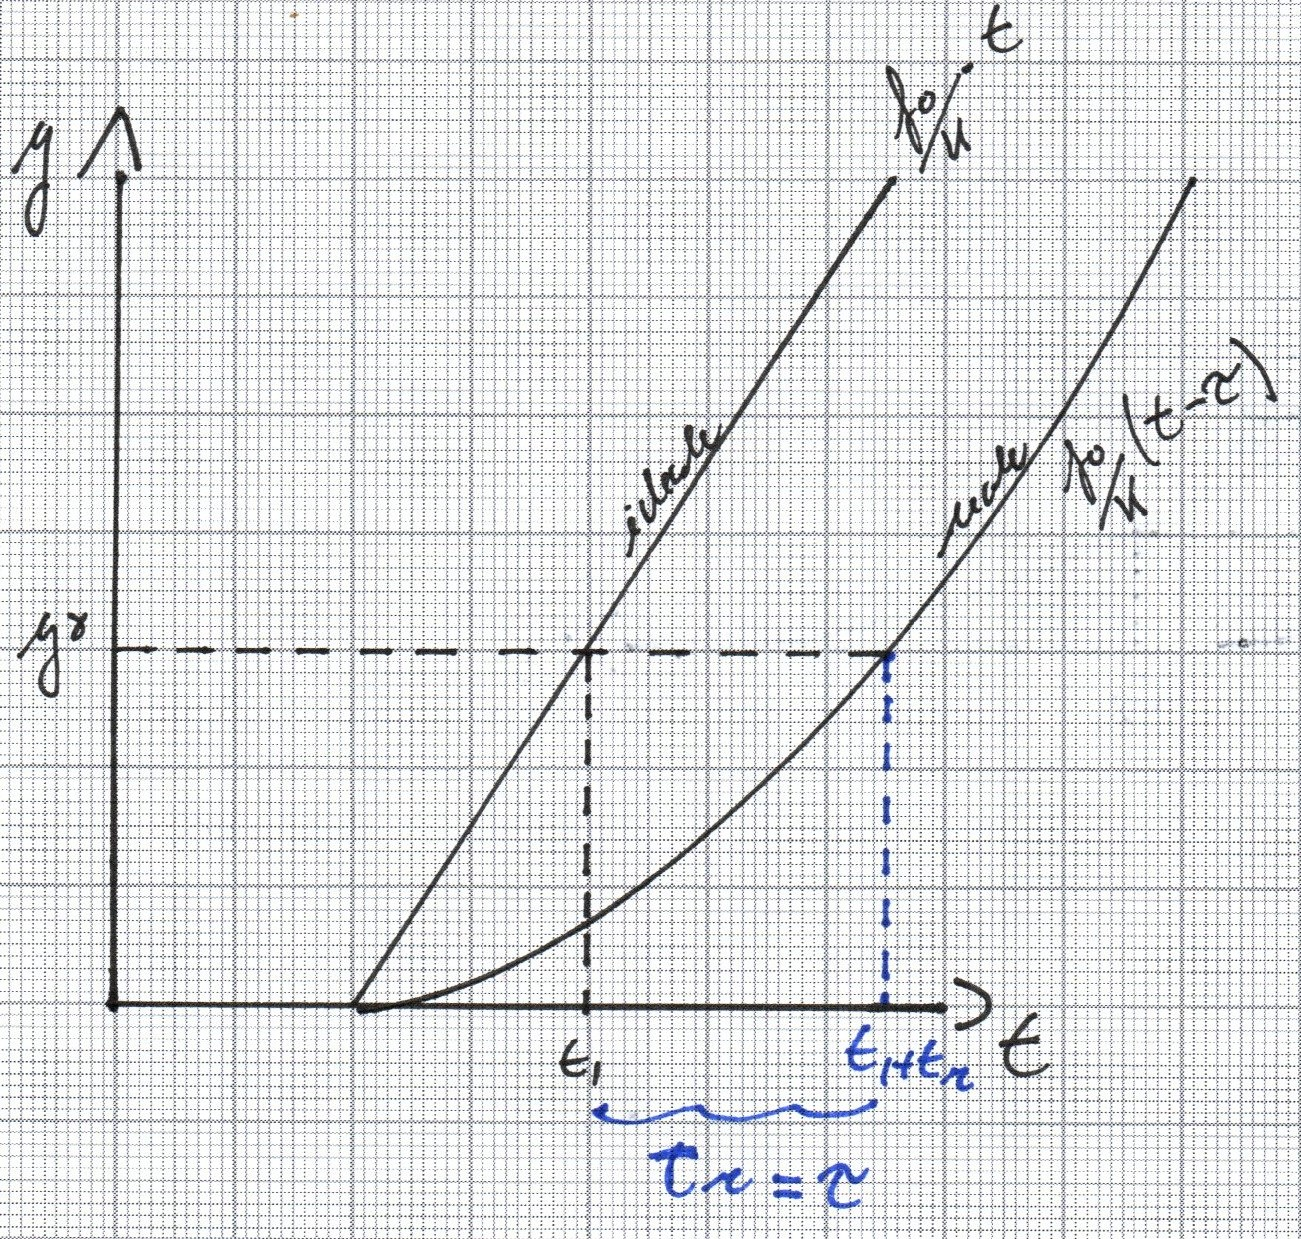
\includegraphics[width=0.4\linewidth]{fig/mm6}
		\label{fig:mm6}
	\end{figure}	
	All'infinito il transitorio si estingue, rimane solo la soluzione particolare, l'andamento a regime, che si discosta dalla retta reale a causa del transitorio esponenziale. \newline
	
	Quant'è il tempo di ritardo tra la soluzione ideale e quella reale?
	\[ y^* = y(t_1) = \dfrac{f_0}{k}t_1 = \dfrac{f_0}{k}[(t_1 + t_r)-\tau] =  y(t_1 + t_r) \]
	\[ \dfrac{f_0}{k}t_1 = \dfrac{f_0}{k}[(t_1 + t_r)-\tau] \]
	\[ t_r = \tau \]
	Il tempo di ritardo non dipende nè da $f_0$ nè dalla pendenza della curva. 
\end{adjustwidth}
%\newpage
\subsection{Ingressi periodici} 	
\begin{adjustwidth}{2in}{}		
	Applico una forza periodica all'elemento. 
	
	Ciò a cui ci si ricondurrà saranno un grafico del guadagno e uno dello sfasamento. 
	\[ c\dot{y}  + ky = F_0\sin(\omega t)\]
	Si è dunque visto come la soluzione omogenea (ormai nota) identifichi sempre il transitorio dello strumento, in questo caso il primo periodo della sinusoide, tale soluzione sarà perciò nulla per tempi elevati ed idealmente infiniti, il che significa che nella seguente trattazione può essere lasciata da parte. \newline 
	
	Si ricavi la soluzione particolare attraverso il metodo dei fasori:
	\[ c\dot{y}  + ky = F_0e^{j\omega t}\]
	Questa sarà nella forma:
	\[y_p = y_0e^{j(\omega t + \varphi)}\]
	Sostituendo:
	\[ cj\omega y_0e^{j(\omega t + \varphi)}  + ky_0e^{j(\omega t + \varphi)} = F_0e^{j\omega t}\]
	\[ y_0e^{j\varphi}(k + cj\omega) = F_0\]
	\[  y_0e^{j\varphi} (1 + \dfrac{j\omega c}{k}) = \dfrac{F_0}{k} \]
	Ricordando che $\tau = c/k$:
	\[  y_0e^{j\varphi} = \dfrac{F_0}{k} \dfrac{1}{1+j\omega \tau} \]
	A cosa mi riconduco? Ad un'uguaglianza tra numeri complessi nella quale $y_0$ mi identifica il modulo e $\varphi$ la fase, il problema ora diventa ricondurre il RHS ad un numero complesso con modulo e fase. \newline 
	
	Razionalizzo il RHS: 
	\[\dfrac{F_0}{k} \dfrac{1}{1+j\omega \tau} \dfrac{1-j\omega \tau}{1-j\omega \tau} = \dfrac{F_0}{k} \dfrac{1-j\omega \tau}{1-(\omega \tau)^2} = \dfrac{F_0}{k[1-(\omega \tau)^2]} \cdot (1-j\omega \tau)  \]
	Riscrivo ora l'uguaglianza da risolvere col metodo di somiglianza:
	\[  y_0e^{j\varphi} = \dfrac{F_0}{k[1-(\omega \tau)^2]} \cdot (1-j\omega \tau) \]
	Al RHS ora è associato il seguente modulo: 
	\[ \sqrt{1+(\omega \tau)^2} \]
	E così: 
	\[ y_0 = \dfrac{F_0}{k[1-(\omega \tau)^2]} \cdot \sqrt{1+(\omega \tau)^2} = \dfrac{F_0}{k}\dfrac{1}{\sqrt{1+(\omega \tau)^2}} \]
	Quali sono i risultati ottenibili da questa formulazione? Si vede immediatamente che il modulo dipende dalla pulsazione $\omega$ da fornire in ingresso, \newline in più per $\omega \rightarrow 0; y_0 \rightarrow \dfrac{F_0}{k}$ mentre per $\omega \rightarrow \infty; y_0 \rightarrow 0$ in completo accordo con il grafico seguente, che non è nient'altro che il grafico del guadagno. 
	
	(Il modulo della soluzione a regime/particolare, è il guadagno?)	
\begin{figure}[H]
	\centering
	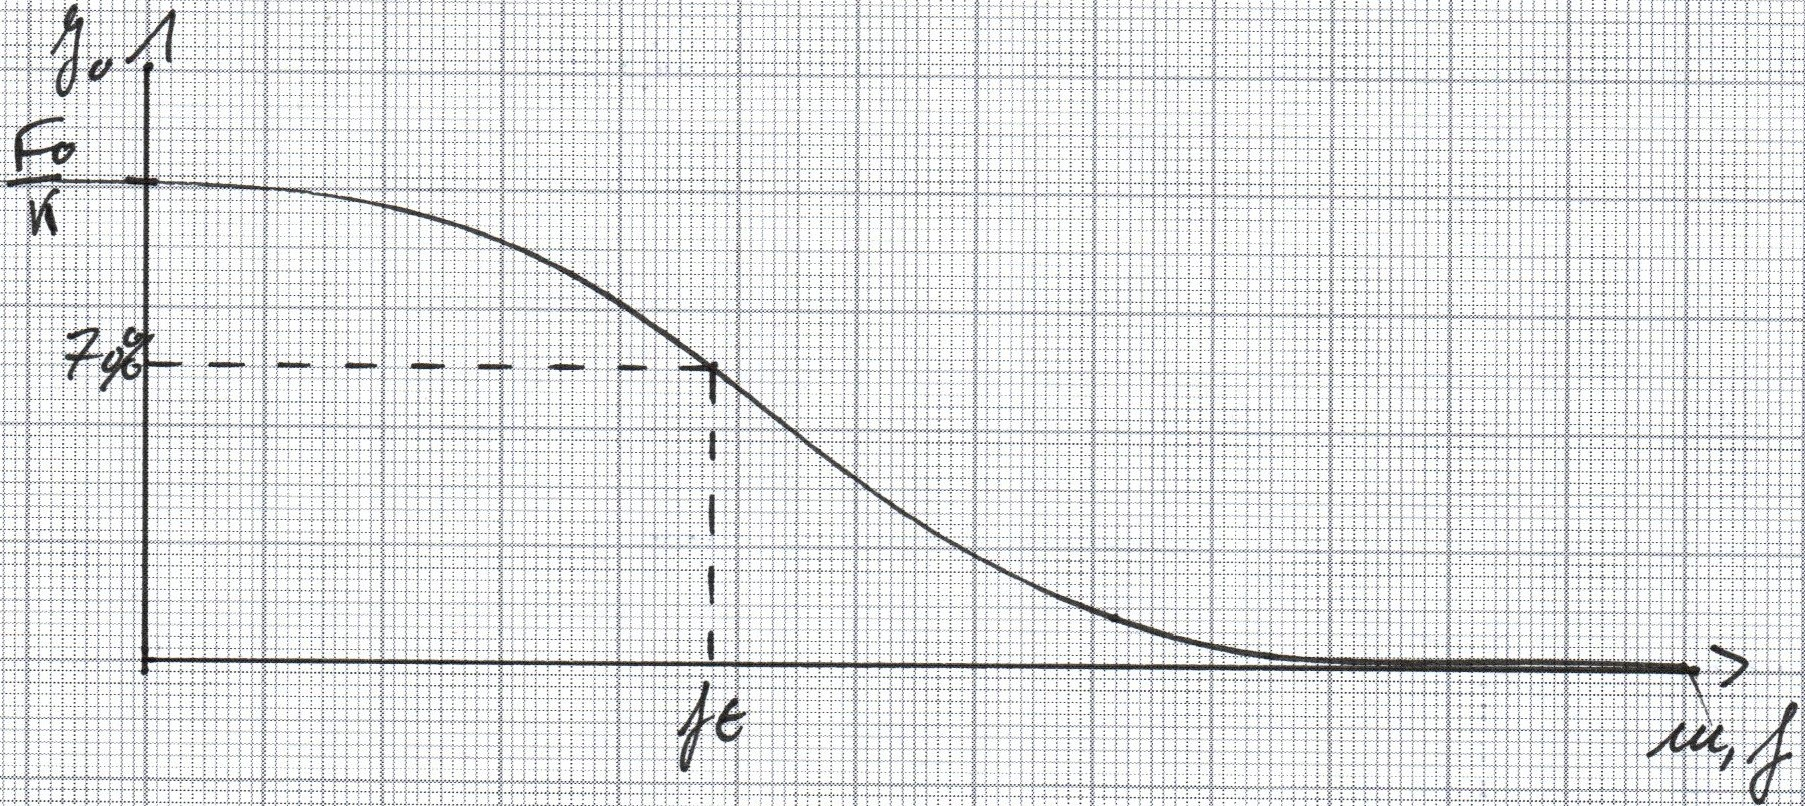
\includegraphics[width=0.5\linewidth]{fig/mm7}
	\label{fig:mm7}
\end{figure}
	Dove posso trovare la frequenza di taglio? 
	\[ -3dB = 20\log_{10}\left[\dfrac{y_{0f}}{y_{00}}\right]\] 
	\[ -3dB = 20\log_{10}\left[\dfrac{\dfrac{F_0}{k}\dfrac{1}{\sqrt{1+(\omega \tau)^2}}}{F_0/k}\right] = 20\log_{10}\left[\dfrac{1}{\sqrt{1+(\omega \tau)^2}}\right] \] 
	Ma
	\[ \left[\dfrac{1}{\sqrt{1+(\omega \tau)^2}}\right] = 0.707 = \dfrac{1}{\sqrt{2}}\]
	
	\[ \dfrac{1}{\sqrt{1+(\omega \tau)^2}} = \dfrac{1}{\sqrt{2}} \]
	\[ \dfrac{1}{1+(\omega \tau)^2} = \dfrac{1}{2} \]	
	\[ 2 = 1+(\omega \tau)^2  \]
	\[ 1 = \omega \tau \]
	\[ \omega_t = \dfrac{1}{\tau}\]
	Infine, poiché:
	\[  \omega_t = 2\pi f_t\]
	La frequenza di taglio sarà: 
	\[  f_t = \dfrac{1}{2\pi\tau}\]
	
	Mentre per la fase? la fase sarà data da:
	\[ \varphi = \arctan(-\omega t) \]
	L'arcotangente tende a $0$ per $f\rightarrow0$ mentre tende a $-\dfrac{\pi}{4}$ per  $f\rightarrow\infty$	
	\begin{figure}[H]
		\centering
		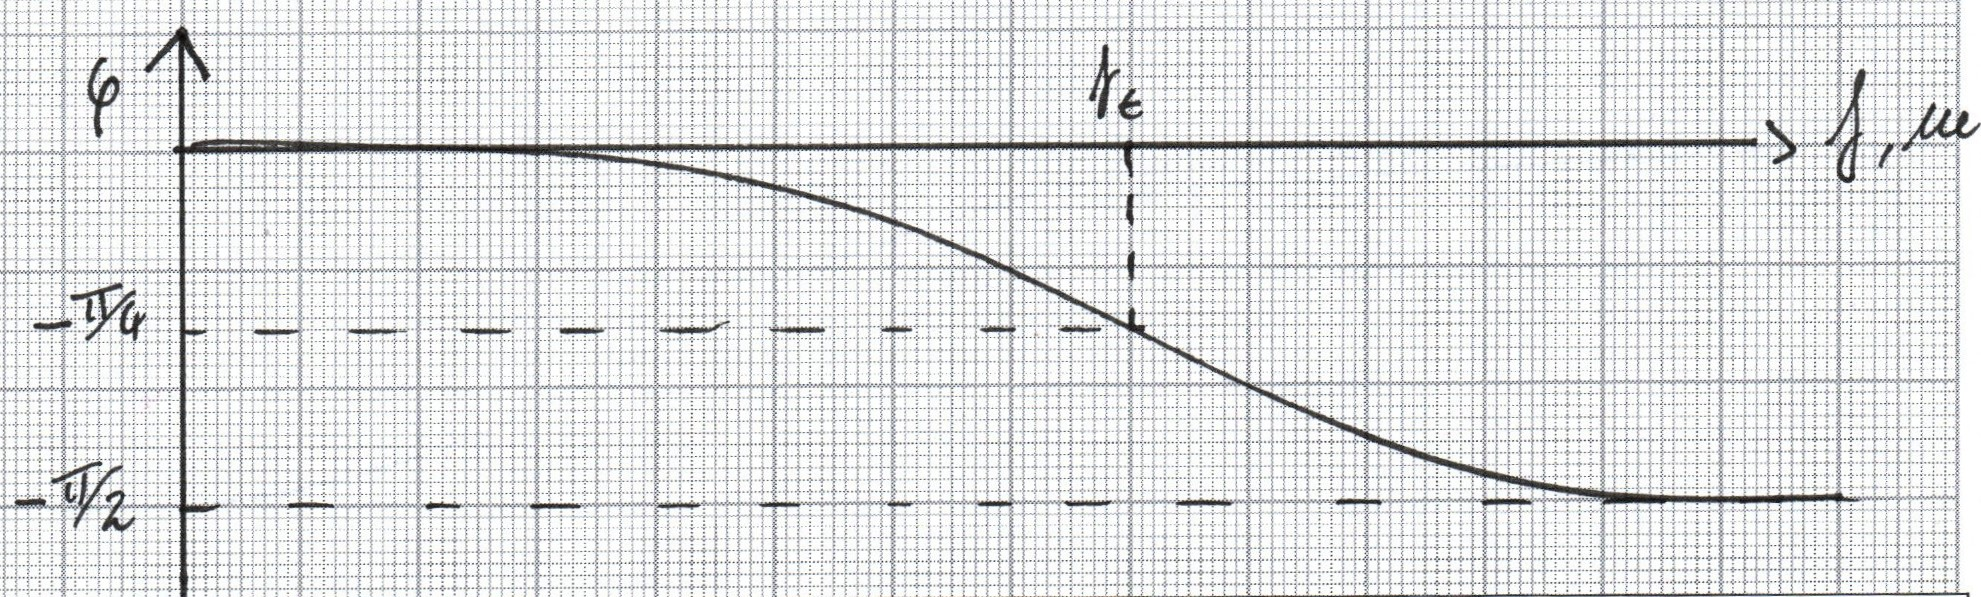
\includegraphics[width=0.5\linewidth]{fig/mm8}
		\label{fig:mm8}
	\end{figure}
\end{adjustwidth}
%\newpage
\subsection{Ricapitolando} 	
\begin{adjustwidth}{2in}{}	
	Quali sono i metodi per il calcolo del $\tau$ per strumenti del primo ordine? 
	\begin{enumerate}
		\item \textbf{Metodo analitico}  
		
		Il calcolo è reso possibile dalla conoscenza di valori noti $y^* = y(t^*)$: 
		\[ y(t) = y_0e^{-t/\tau} \Rightarrow y(t^*) = y_0e^{-t^*/\tau} \]
		\[  \dfrac{y^*}{y_0} = e^{-t^*/\tau} \Rightarrow \tau = \dfrac{-t^*}{\log \left[\dfrac{y^*}{y_0}\right]}\]
		
		\item \textbf{Primo metodo grafico} 
		
		È una prova sperimentale per la quale, data la curva, si calcolano per $n$ punti, $(y_1, t_1); (y_2, t_2); \dots (y_n, t_n)$ e si ricavano le rispettive $\tau_1; \tau_2; \dots \tau_n$, il valore finale della $\tau$ sarà la media dei valori così ottenuti.
		
		\item \textbf{Secondo metodo grafico: sottotangenti} 
		 
		Anche qua l'obbiettivo è quello di trovare tanti più $\tau$ possibili ma stavolta col metodo delle sottotangenti per cui il valore finale sarà la media dei valori ottenuti.

		\item \textbf{Terzo metodo grafico}
		
		In questo metodo di sfrutta la funzione di ingresso a gradino sapendo che per il gradino discendente e crescente $\tau$ si trova rispettivamente al $37\%$ e al $63\%$ del valore totale.
		
		\item \textbf{Quarto metodo grafico} 
		
		Sfrutto l'ingresso a rampa per calcolare il $\tau$, che in questo caso sarà proprio uguale al tempo di riposo. 
		
		\item \textbf{Attraverso il grafico del guadagno} 
		
		In questo metodo, data una serie di seni, calcolo per tutti e per punti l'andamento in frequenza da plottare. 
		
		Trovo la frequenza o la pulsazione di taglio e il $\tau$ sarà presto determinato: 
		\[\omega_t = \dfrac{1}{\tau} \hspace{1cm}  f_t = \dfrac{1}{2\pi\tau} \]	
		Oltre al fatto che:
		\[0.7G_0 = \dfrac{1}{\tau}\]	
	\end{enumerate}
\end{adjustwidth}
\newpage
\subsubsection{Termometro a bulbo}	
\begin{adjustwidth}{2in}{}
	Un esempio di strumento del primo ordine è un termometro a bulbo che viene rapidamente inserito in un ambiente a $T_a$. 
	\begin{figure}[H]
		\centering
		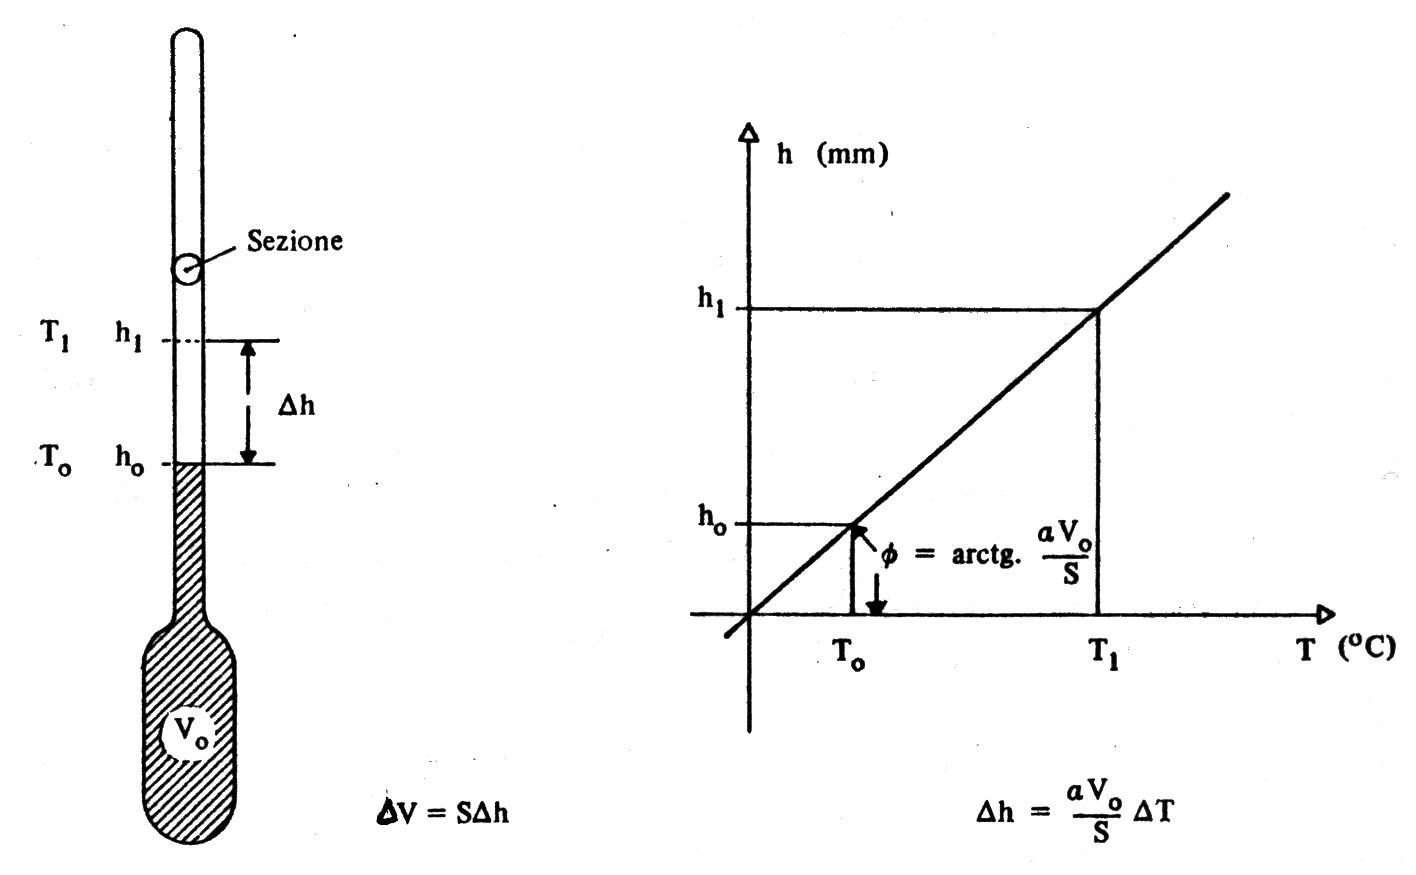
\includegraphics[width=0.7\linewidth]{fig/imag3}
		\label{fig:imag3}
	\end{figure}	
	A livello statico si era visto che:
	\[ \Delta h = \dfrac{\alpha V}{A}\Delta T \hspace{1cm} S = \dfrac{\alpha V}{A} \]
	Lo scambio termico termico con l'ambiente è regolate dalle seguenti equazioni: 
	\[  \begin{cases}
		dQ = kA_s(T_a - T)dt \\
		dQ = mcdT 
	\end{cases}\]
	In cui $A_s$ è l'area di scambio termico. 
	
	Il calore scambiato con l'ambiente dev'essere uguale a quello assorbito dal fluido all'interno del termometro, per cui:
	\[ kA_s(T_a - T)dt = mcdT \]
	\[ (T_a - T) = \dfrac{mc}{kA_s}\dfrac{dT}{dt}\]
	\[ \dfrac{mc}{kA_s}\dfrac{dT}{dt} + T = T_a  \]
	Come nelle equazioni viste fin'ora, ci si è ricondotti ad una forma:
	\[ c\dot{y} + ky = F_0\]
	Essendo $ \tau = c/k $, in questo caso 
	\[\tau = \dfrac{mc}{kA_s}/1 = \dfrac{mc}{kA_s}\]
\end{adjustwidth}
%\newpage
\subsubsection{Considerazioni finali}	
\begin{adjustwidth}{2in}{}	
	Si conclude con alcune considerazioni: un $\tau$ picciolo comporta uno strumento più rapido ma per ottenerlo si deve diminuire la massa del fluido o la superficie di scambio termico, ma questo significherebbe diminuire anche la sensibilità dello strumento, d'alta parte uno strumento molto sensibili presenta un volume di fluido più elevato che va ad innalzare giocoforza la massa e dunque ad innalzare il $\tau$. 
	
	Spesso le caratteristiche metrologiche dinamiche cozzano con quelle statiche. \newline 
	
	Si preferisce quindi manipolare i fluidi in modo che i coefficienti $c, \alpha$ siano alti e il coefficiente $k$ sia basso.  
\end{adjustwidth}
\newpage
\section{Strumento di ordine $II$}	
\begin{adjustwidth}{2in}{}	 
	\begin{figure}[H]
		\centering
		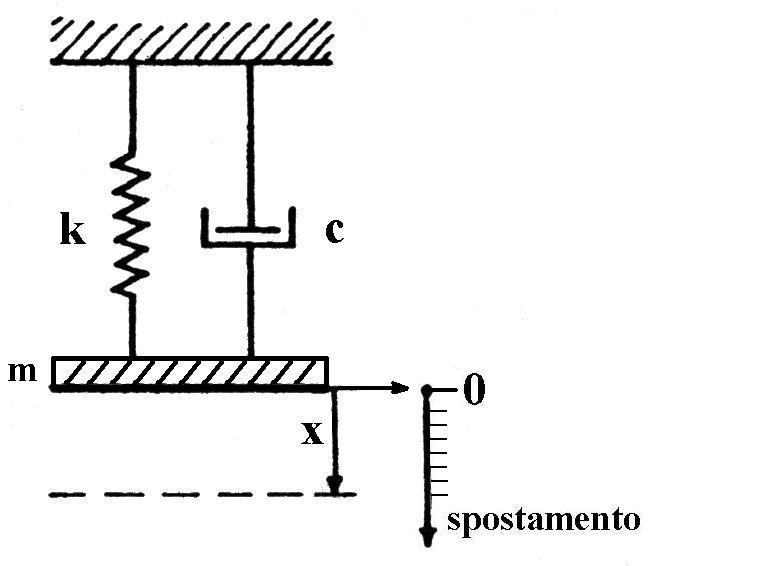
\includegraphics[width=0.5\linewidth]{fig/imag4}
		\label{fig:imag4}
	\end{figure}
	La differenza con gli strumenti del $I$ ordine ora risiede nel considerare la massa dell'oggetto e quindi la sua forza peso, l'equazione differenziale vista negli strumenti del primo ordine si modificherà aggiungendo una forza e dunque la massa per l'accelerazione dell'oggetto. 
	\[ M\ddot{y} + c\dot{y} + ky = F(t)\]
	
	\begin{center}
		\textbf{Esattamente come negli strumenti del primo ordine si analizzeranno i vari ingressi.}
	\end{center}  
\end{adjustwidth}
%\newpage
\subsection{Gradino decrescente} 	
\begin{adjustwidth}{2in}{} 	
	Come si ottiene un gradino decrescente? Si pone l'oggetto avere un allungamento ${F_0\over k}$, lo si blocca in quella posizione e poi si taglia il supporto facendolo ritornare nella posizione di partenza.
	
	L'equazione diviene così:
	\[ M\ddot{y} + c\dot{y} + ky =0\]
	Alla quale dovranno essere aggiunte due equazioni al contorno:
	\[ \begin{cases}
		y(0)=F_0/k \\
		\dot{y}(0) = F_0
	\end{cases}\]
	La soluzione nota è: 
	\[ y(t)=Ae^{\alpha t}\]
	Quanto vale $\alpha$? Sostituisco:
	\begin{eqnarray*}
		MA\alpha^2e^{\alpha t} + cA\alpha e^{\alpha t} + kAe^{\alpha t}  = 0 \\
		M\alpha^2 + c\alpha + k = 0 \\
		\Leftrightarrow \\
		\alpha  =\dfrac{-c \pm \sqrt{c^2 - 4Mk}}{2M}
	\end{eqnarray*}
	Si introducono due parametri:
	\begin{itemize}
		\item \textbf{Pulsazione naturale}: \(\omega_n = \sqrt{k\over M}\)
		\item \textbf{Fattore di smorzamento}: \( \xi = \dfrac{c}{\sqrt{kM}}\)
	\end{itemize}
	E allora si può scrivere \[c = 2\sqrt{kM}\xi\]
	\newpage
	E quindi
	\[ \begin{split}
		\alpha & = -{c\over 2M} \pm \sqrt{{c^2\over 4M^2} - {4Mk\over 4M^2}} = -{c\over 2M} \pm \sqrt{{c^2\over 4M^2} - {k\over M}} = \\
		& = -{2\sqrt{kM}\xi\over 2M} \pm \sqrt{{4kM\xi^2\over 4M^2} - {k\over M}} = -\sqrt{k\over M} \pm \sqrt{{k\over M}\xi^2 - {k\over M}} =  \\
		& = -\omega_n\xi \pm \sqrt{\omega^2_n\xi^2 - \omega^2_n} 
	\end{split} \]
	Infine si avrà:
	\[\alpha_{1,2}= -\omega_n\xi \pm \omega_n\sqrt{\xi^2 - 1}\]
	Col risultato che $\alpha$ varia in funzione di $\xi$, che questo sia maggiore, uguale o minore di $1$ si avranno diverse soluzioni e diverse tipologie di smorzamento.  
	\begin{enumerate}[label=(\Roman*)]
	\item \textbf{Caso $\xi>1$: Soluzioni reali distinte}
	\begin{eqnarray*}
		y(t) = A_1e^{\alpha_1 t} + A_2e^{\alpha_2 t} \\
		\dot{y}(t) = A_1\alpha_1e^{\alpha_1 t} + A_2\alpha_2e^{\alpha_2 t}
	\end{eqnarray*}  
	Imponendo le condizioni al contorno ottengo:
	\[ \begin{cases}
		y(0) = A_1 + A_2 = {F_0 \over k } \\
		\dot{y}(t) = A_1\alpha_1 + A_2\alpha_2 = 0
	\end{cases}\]
	Un sistema lineare di due equazioni in due incognite. 	
\begin{figure}[H]
	\centering
	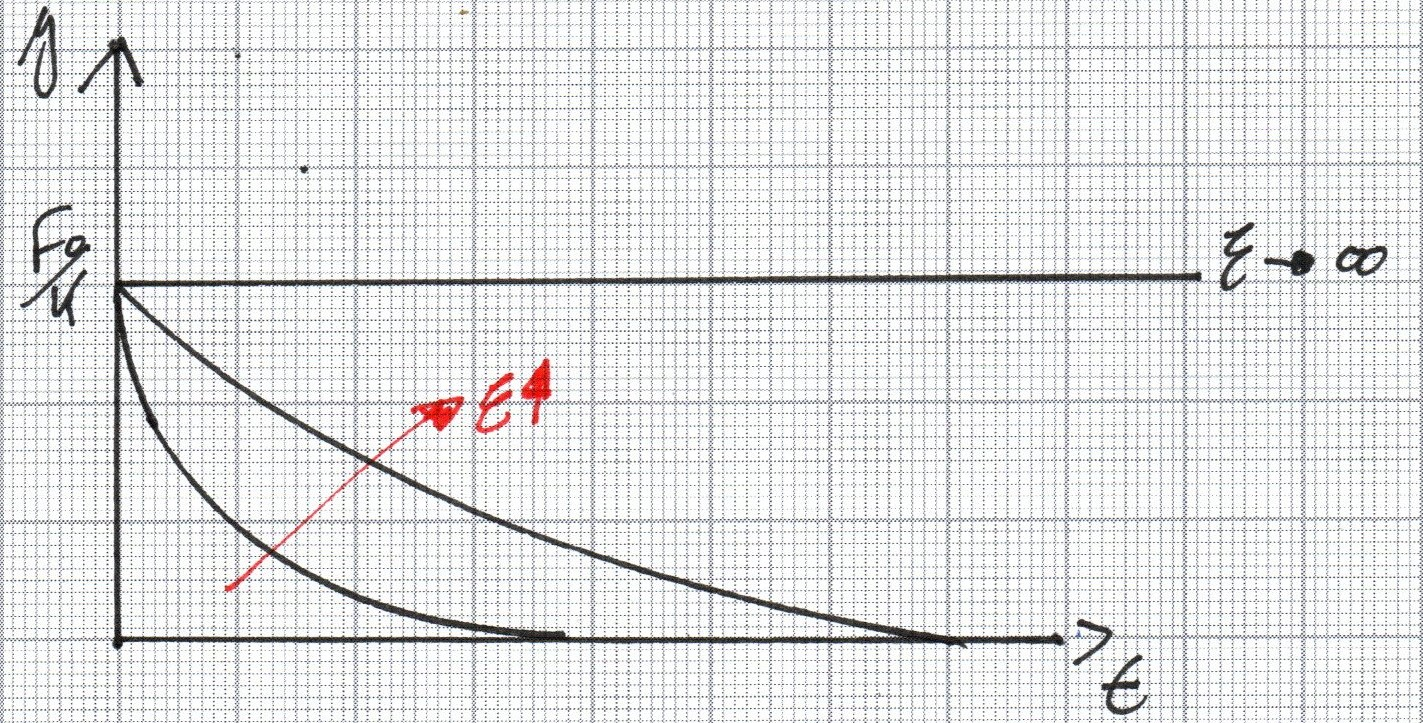
\includegraphics[width=0.5\linewidth]{fig/mm9}
	\label{fig:mm9}
\end{figure}	
	\item \textbf{Caso $\xi=1$: Soluzioni reali coincidenti} \(\alpha_{1,2} = -\omega_n\) \newline
	\begin{eqnarray*}
		y(t) = A_1e^{-\omega_n t} + A_2te^{-\omega_n t} \\
		\dot{y}(t) = -\omega_nA_1e^{-\omega_n t} + A_2\left(-\omega_nte^{-\omega_n t} - e^{-\omega_n t}\right)
	\end{eqnarray*}
	Imponendo le condizioni al contorno ottengo:
	\[ \begin{cases}
		y(0) = A_1 = {F_0 \over k } \\
		\dot{y}(t) = -\omega_nA_1\alpha_1 + A_2\alpha_2 = 0
	\end{cases}\]
	Il grafico che si ottiene è quello la curva più interna di qualsia altra prima ottenuta fin'ora.  	
\begin{figure}[H]
	\centering
	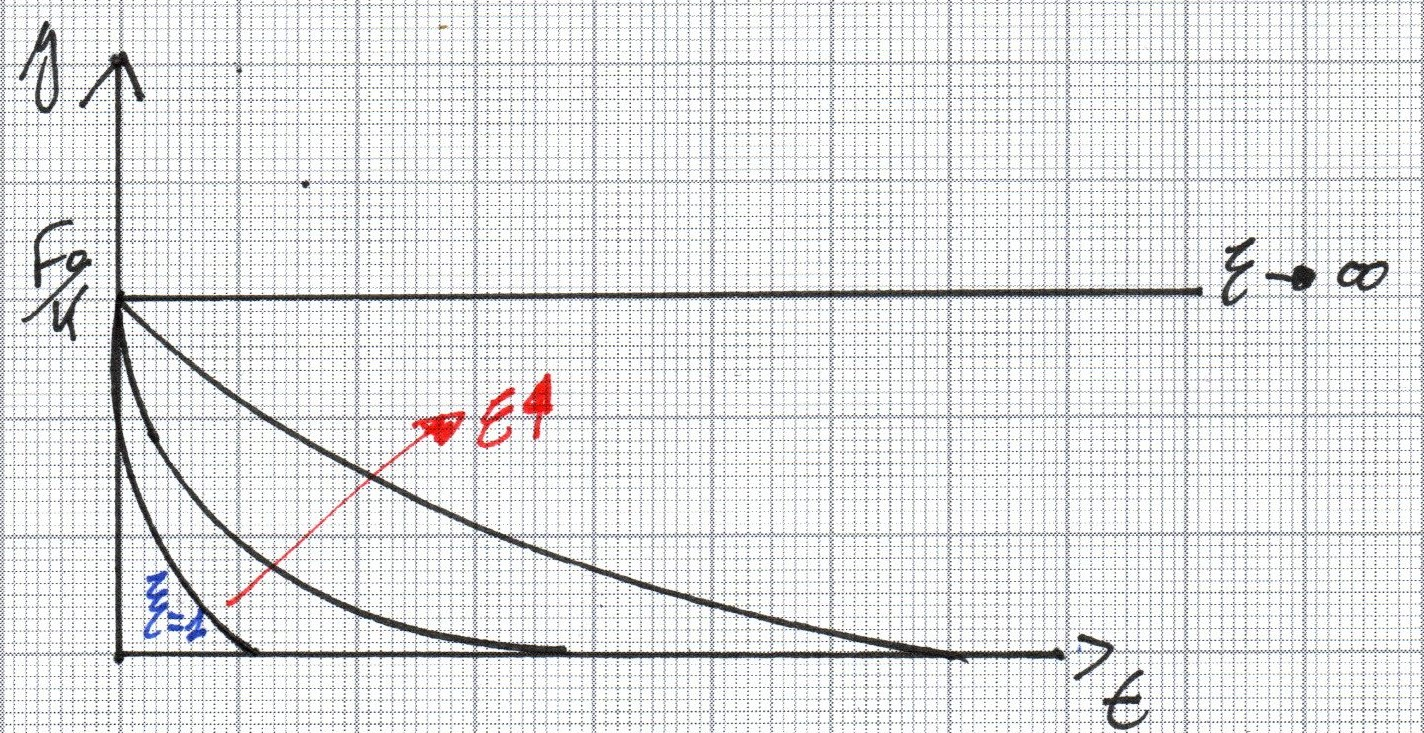
\includegraphics[width=0.5\linewidth]{fig/mm10}
	\label{fig:mm10}
\end{figure}
	\item \textbf{Caso $\xi<1$: Soluzioni complesse}  
	\begin{eqnarray}
		\alpha_{1,2}= -\omega_n\xi \pm j\omega_n\sqrt{1 - \xi^2} \\
		y(t) = A_1e^{-\omega_n\xi t}e^{j\sqrt{1 - \xi^2}+ t}  A_2e^{-\omega_n\xi t}e^{-j\sqrt{1 - \xi^2}} \\
		y(t) = Ae^{-\omega_n\xi t}\sin(\omega_n\sqrt{1 - \xi^2}t + \varphi)
	\end{eqnarray}
	Introducendo la pulsazione propria del sistema \( \omega_0 = \omega_n\sqrt{1 - \xi^2} \):
	\[y(t) = Ae^{-\omega_n\xi t}\sin(\omega_0t + \varphi)\]
	I grafici che si ottengono saranno i seguenti: 
\begin{figure}[H]
	\centering
	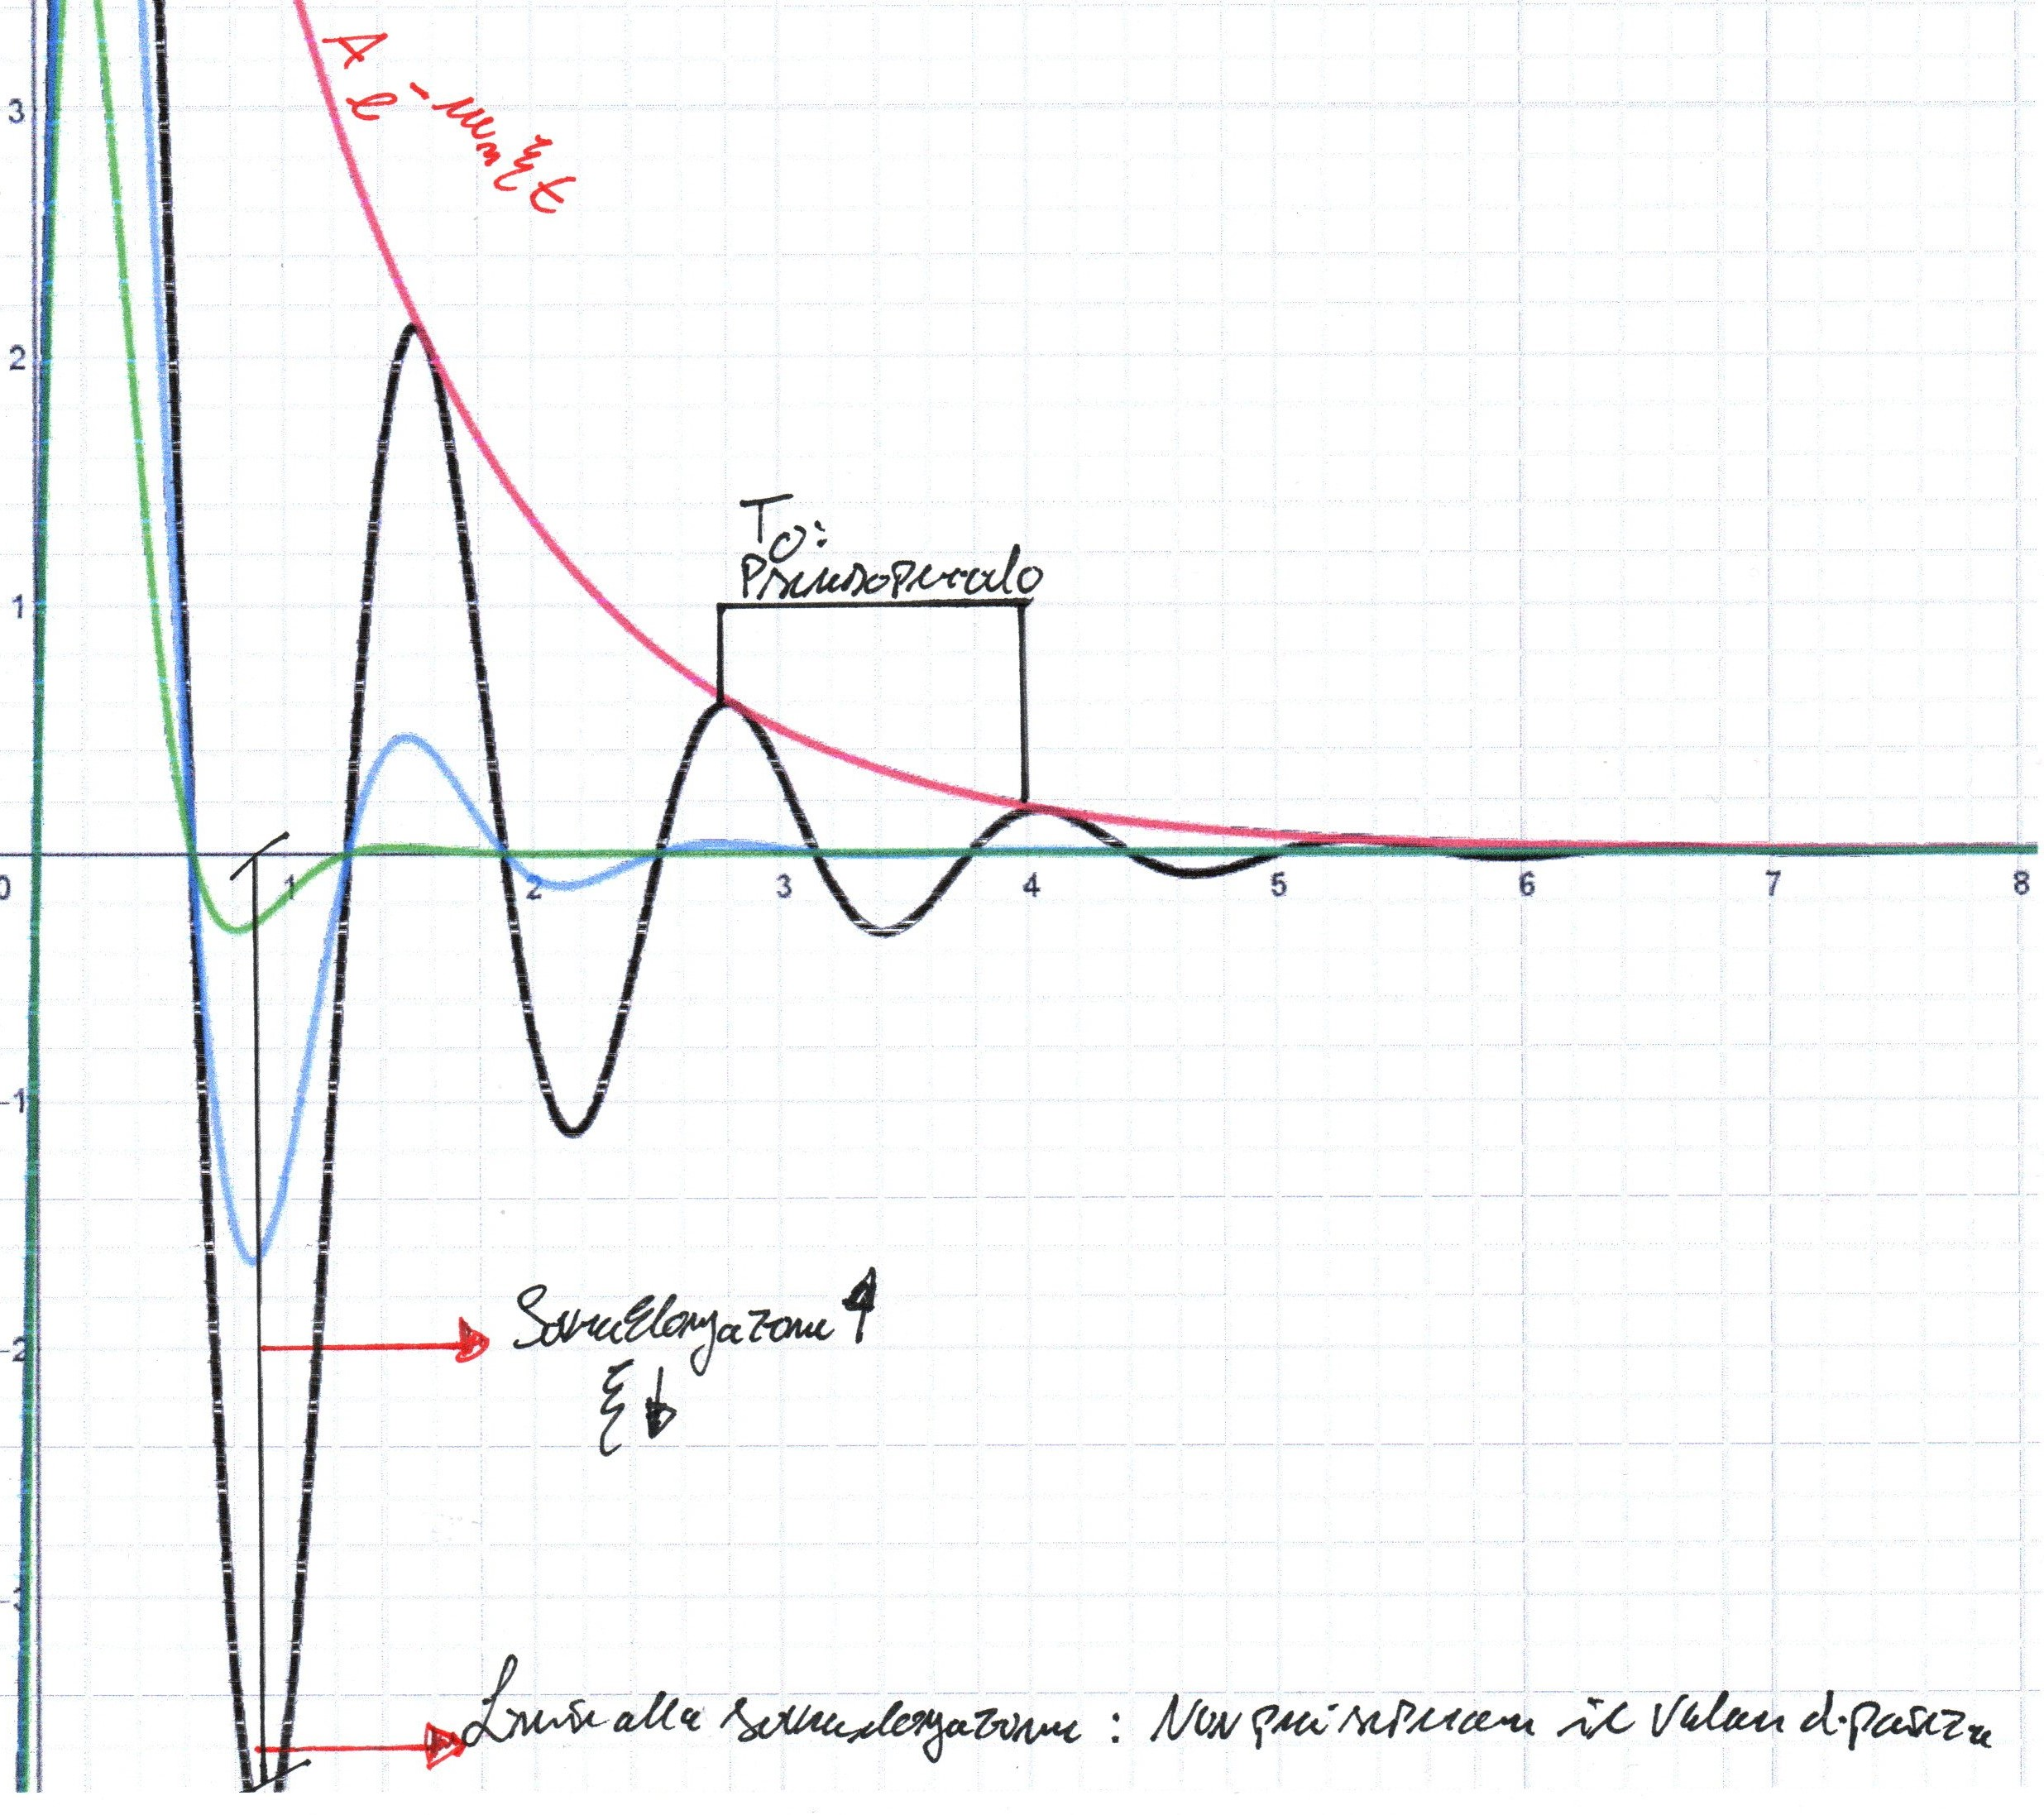
\includegraphics[width=0.5\linewidth]{fig/mm11}
	\label{fig:mm11}
\end{figure}
	NB: la sovraelongazione non può andare oltre al valore di partenza, c'è sempre un $\sin$ che nel peggiore dei casi può valere $-1$. 
	
	Introduco lo pseudoperiodo $T_0$ come il periodo tra due oscillazioni, tenendo conto che la funzione non è una sinusoidale pura. \newline 
	
	Dagli andamenti inoltre si nota che, come $\xi$ cresce la sovraelongazione diminuisce ed il periodo aumenta, mentre viceversa, come $\xi$ diminuisce la sovraelongazione aumenta ed il periodo diminuisce. \newline 
	
	\item \textbf{E se $\xi=0$}? 
	
	Varrà
	\[ \omega_0 = \omega_n\] 
	E quindi 
	\[y(t) = A\sin(\omega_nt + \varphi)\]
	Non c'è smorzamento. 
	\[ \dot{y}(t) = A\omega_n\cos(\omega_nt + \varphi)\]
	Applicando le condizioni al contorno si ottiene: 
	\[\begin{cases}
		y(0) = {F_0\over k} = A\sin\varphi \\
		\dot{y}(0) = 0 = A\omega_n\cos\varphi
	\end{cases} \hspace{0.5cm} \begin{cases}
		0 = A\omega_n\cos\varphi \Leftrightarrow \varphi = {\pi\over2} \\
		{F_0\over k} = A\sin\varphi \Leftrightarrow A =  {F_0\over k}
	\end{cases} \]
	Infine:
	\[y(t) = {F_0\over k}\sin(\omega_nt + {\pi\over2})\]
	Oppure, equivalentemente:
	\[y(t) = {F_0\over k}\cos(\omega_nt)\]
	È irrealistico, il grafico non presenta smorzamento.
	
	Il grafico è una cosinusoide pure che non presenta smorzamento, e quindi ha un tempo di stabilizzazione infinito, oscilla tra \[\pm{F_0\over k}\]
\end{enumerate}
\end{adjustwidth}
%\newpage
\subsubsection{Scelta del valore di $\xi$} 	
\begin{adjustwidth}{2in}{} 		
	Diviene così di vitale importanza la scelta del paramento $\xi$: qual è il suo miglior valore? \newline
	
	Si è appena visto come questo debba obbligatoriamente essere non nullo, ma di quanto? Me lo dicono l'errore rispetto al quale è accettabile quella misura e il tempo che sono disposto ad attendere prima che il risultato sia disponibile senza errori, ovvero rispettivamente la banda di errore dinamico $\varepsilon_d$ ed il tempo di stabilizzazione $T_{st}$, tempo impiegato ad entrare in $\varepsilon_d$ e non uscire più.
\begin{figure}[H]
	\centering
	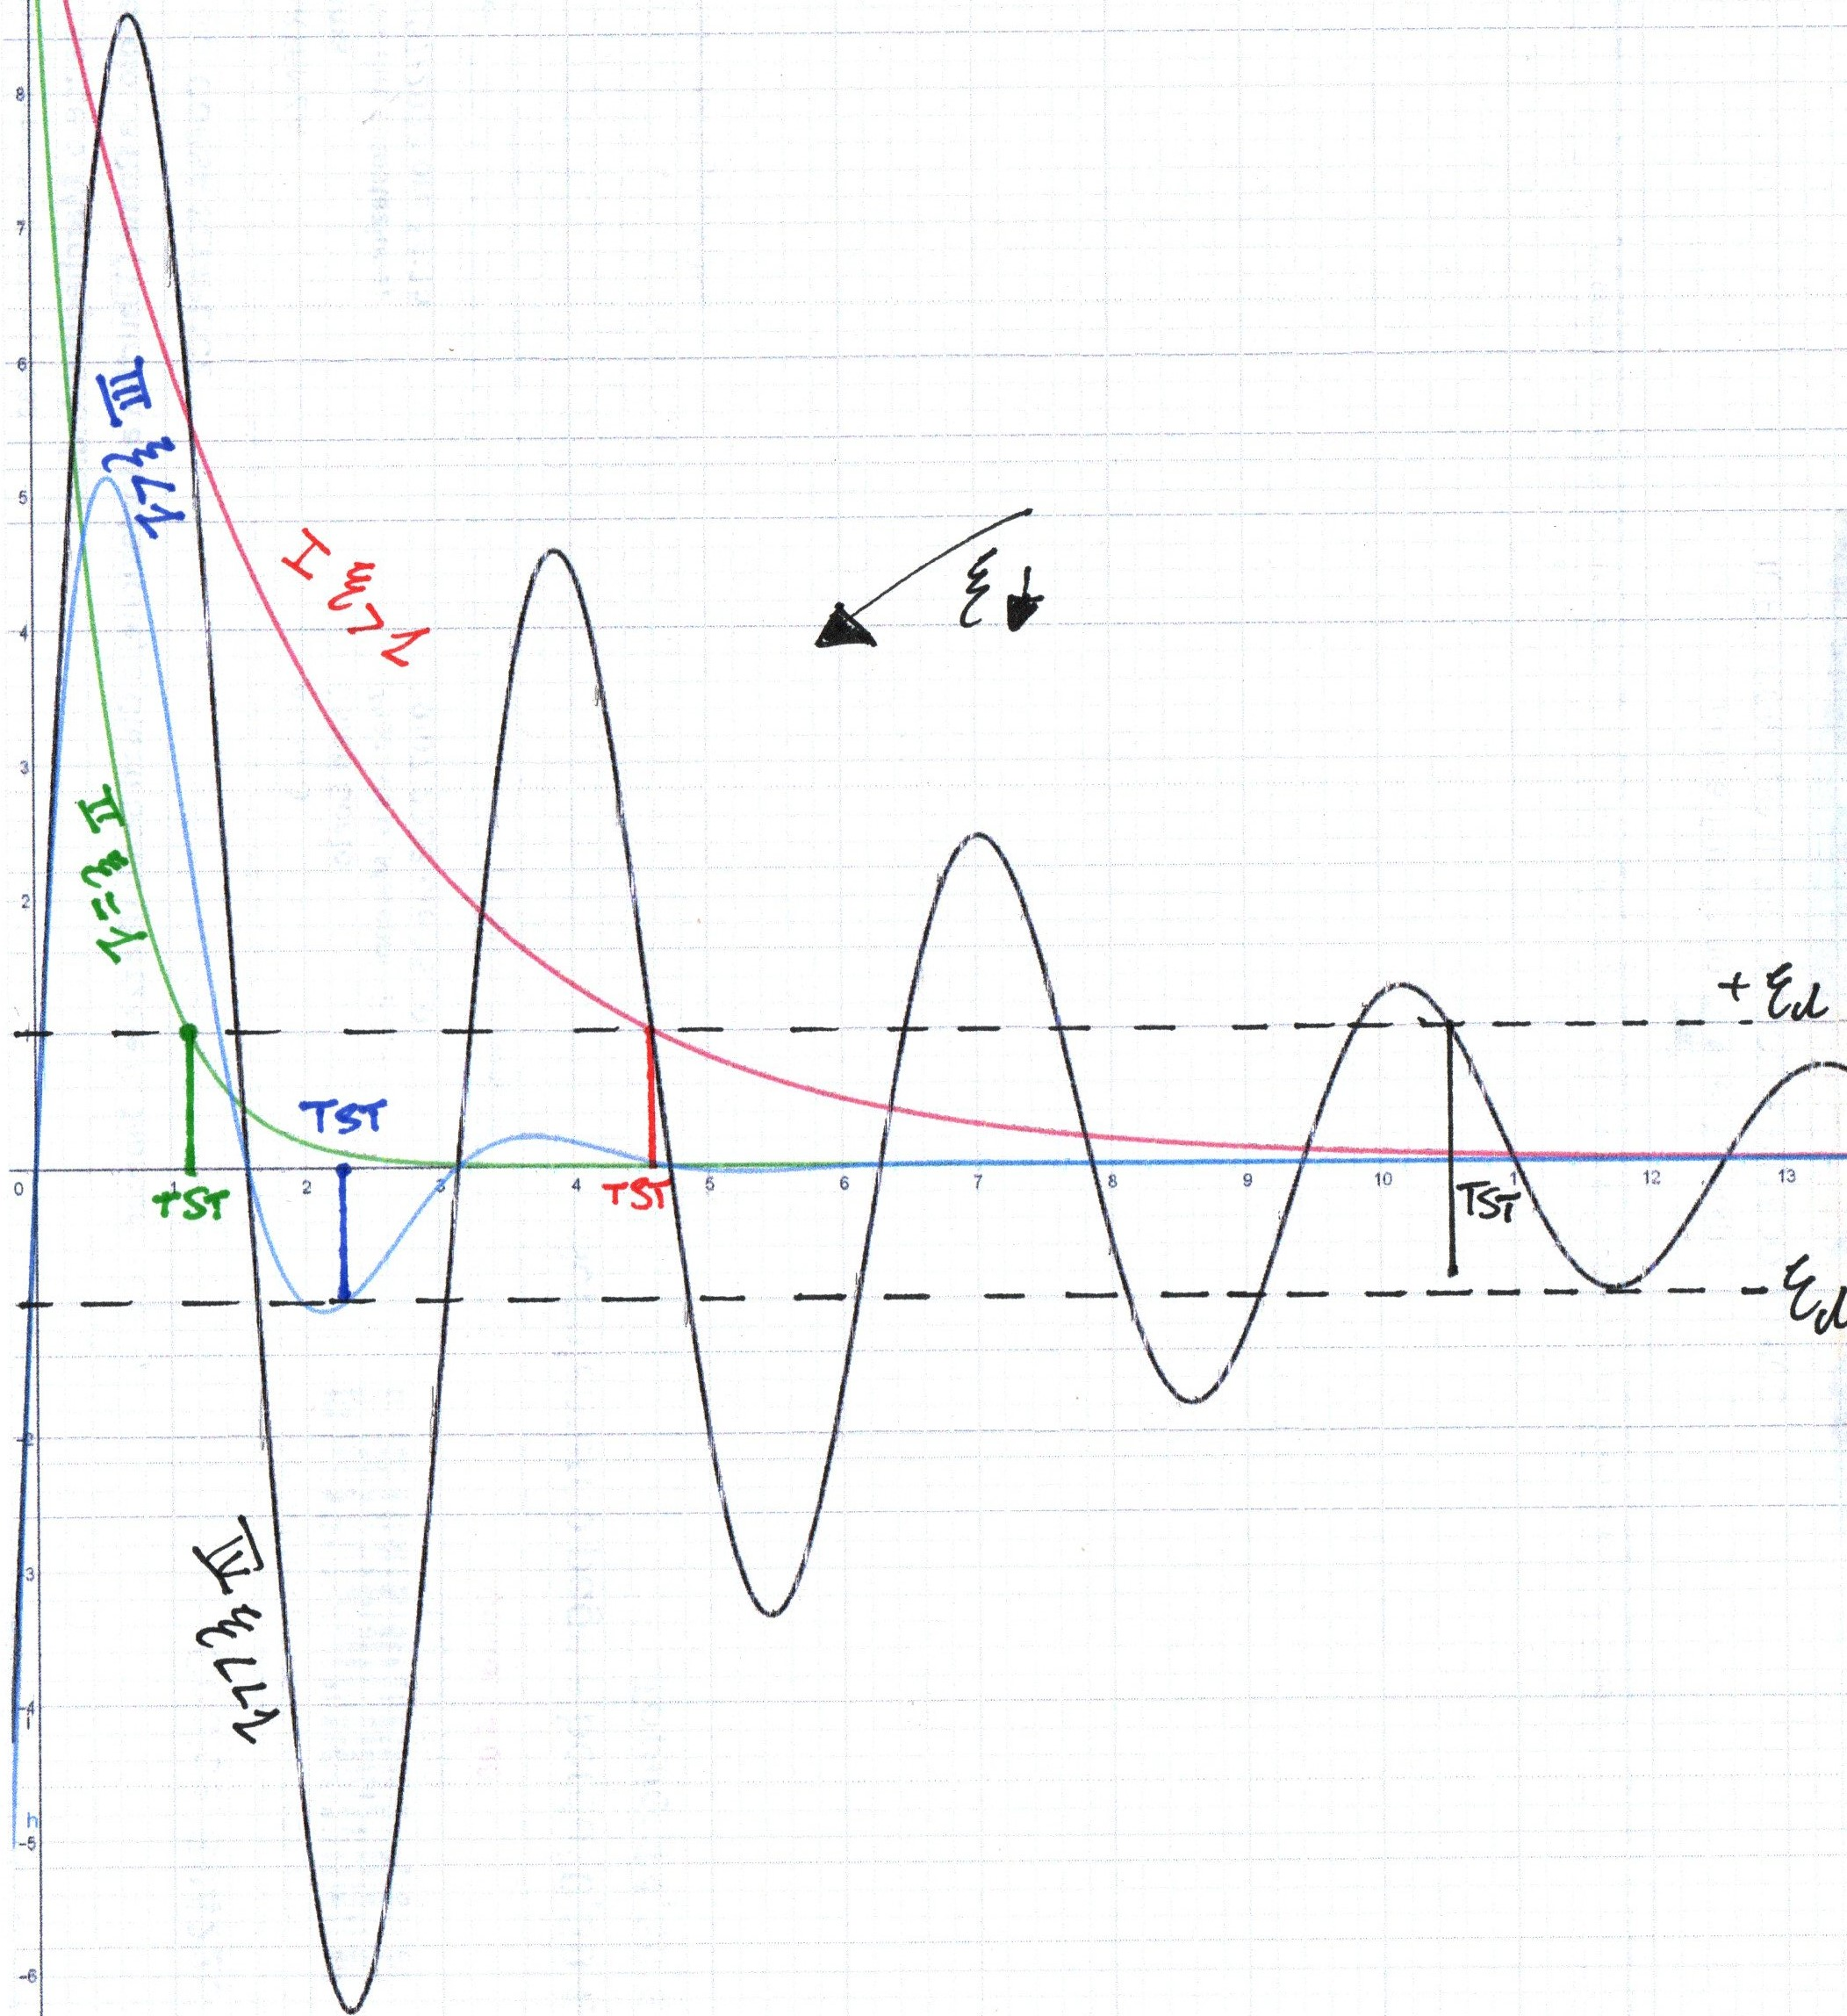
\includegraphics[width=0.5\linewidth]{fig/mm12}
	\label{fig:mm12}
\end{figure}
	Al diminuire di $\xi$ si percorrono via via esponenziali più veloci, fino ad arrivare a quella identificata da $\xi=1$, la più veloce. 

	\begin{enumerate}[label=\Roman*.]
	\item impiega molto tempo ad arrivare a $0$ e ad entrare in $\varepsilon_d$.
	
	\item impiega meno tempo ad arrivare a $0$ e ad entrare in $\varepsilon_d$.
	
	\item impiegherebbe ancor meno tempo ad entrare in $\varepsilon_d$ (in funzione della frequenza), ma presenta una sovraelongazione, siamo nel campo $\xi<1$. \newline
	
	Si potrebbe perciò pensare che continuando a diminuire $\xi\ll1$ incontreremmo tempi di stabilizzazione ancor minori. Nulla di più sbagliato. 
	
	\item Aumentando la sovraelongazione la risposta non entra più immediatamente all'interno della banda di $\varepsilon_d$, ma entra ed esce, entra ed esce, e il tempo di stabilizzazione aumenta rendendo inefficace la trattazione.
	\end{enumerate}  
	
	Devo scegliere un $\xi$ che mi permetta di entrare subito nella banda di errore dinamico e permanerci il più possibile il prima possibile, come in $III$, empiricamente e sperimentamene si sceglie un valore pari a: 
	\[\xi = 0.7\]
\end{adjustwidth}
\newpage
\subsection{Metodo grafico per la determinazione di $\xi$ ed $\omega_n$} 
\subsubsection{Decremento logaritmico}	
\begin{adjustwidth}{2in}{} 	
	\textbf{Valido solo per $\xi<1$.} 
	
	La soluzione dell'equazione era: 
	\[ y(t) = Ae^{-\omega_n\xi t}\sin(\omega_nt + \varphi)\]
	L'inviluppo dei massimi è fornito dall'equazione:
	\[ y(t) =  Ae^{-\omega_n\xi t} \]	
	Si prendano due massimi di ordine diverso, a titolo d'esempio $y_{M,i}, y_{M,i+n}$, in modo che la distanza tra i massimi sia $n$ (per un massimo dopo l'altro $n=1$), si ricordi poi la definizione di periodo $T_0$ in modo che, la distanza tra i due massimi prima considerati sia proprio $nT_0$. 
\begin{figure}[H]
	\centering
	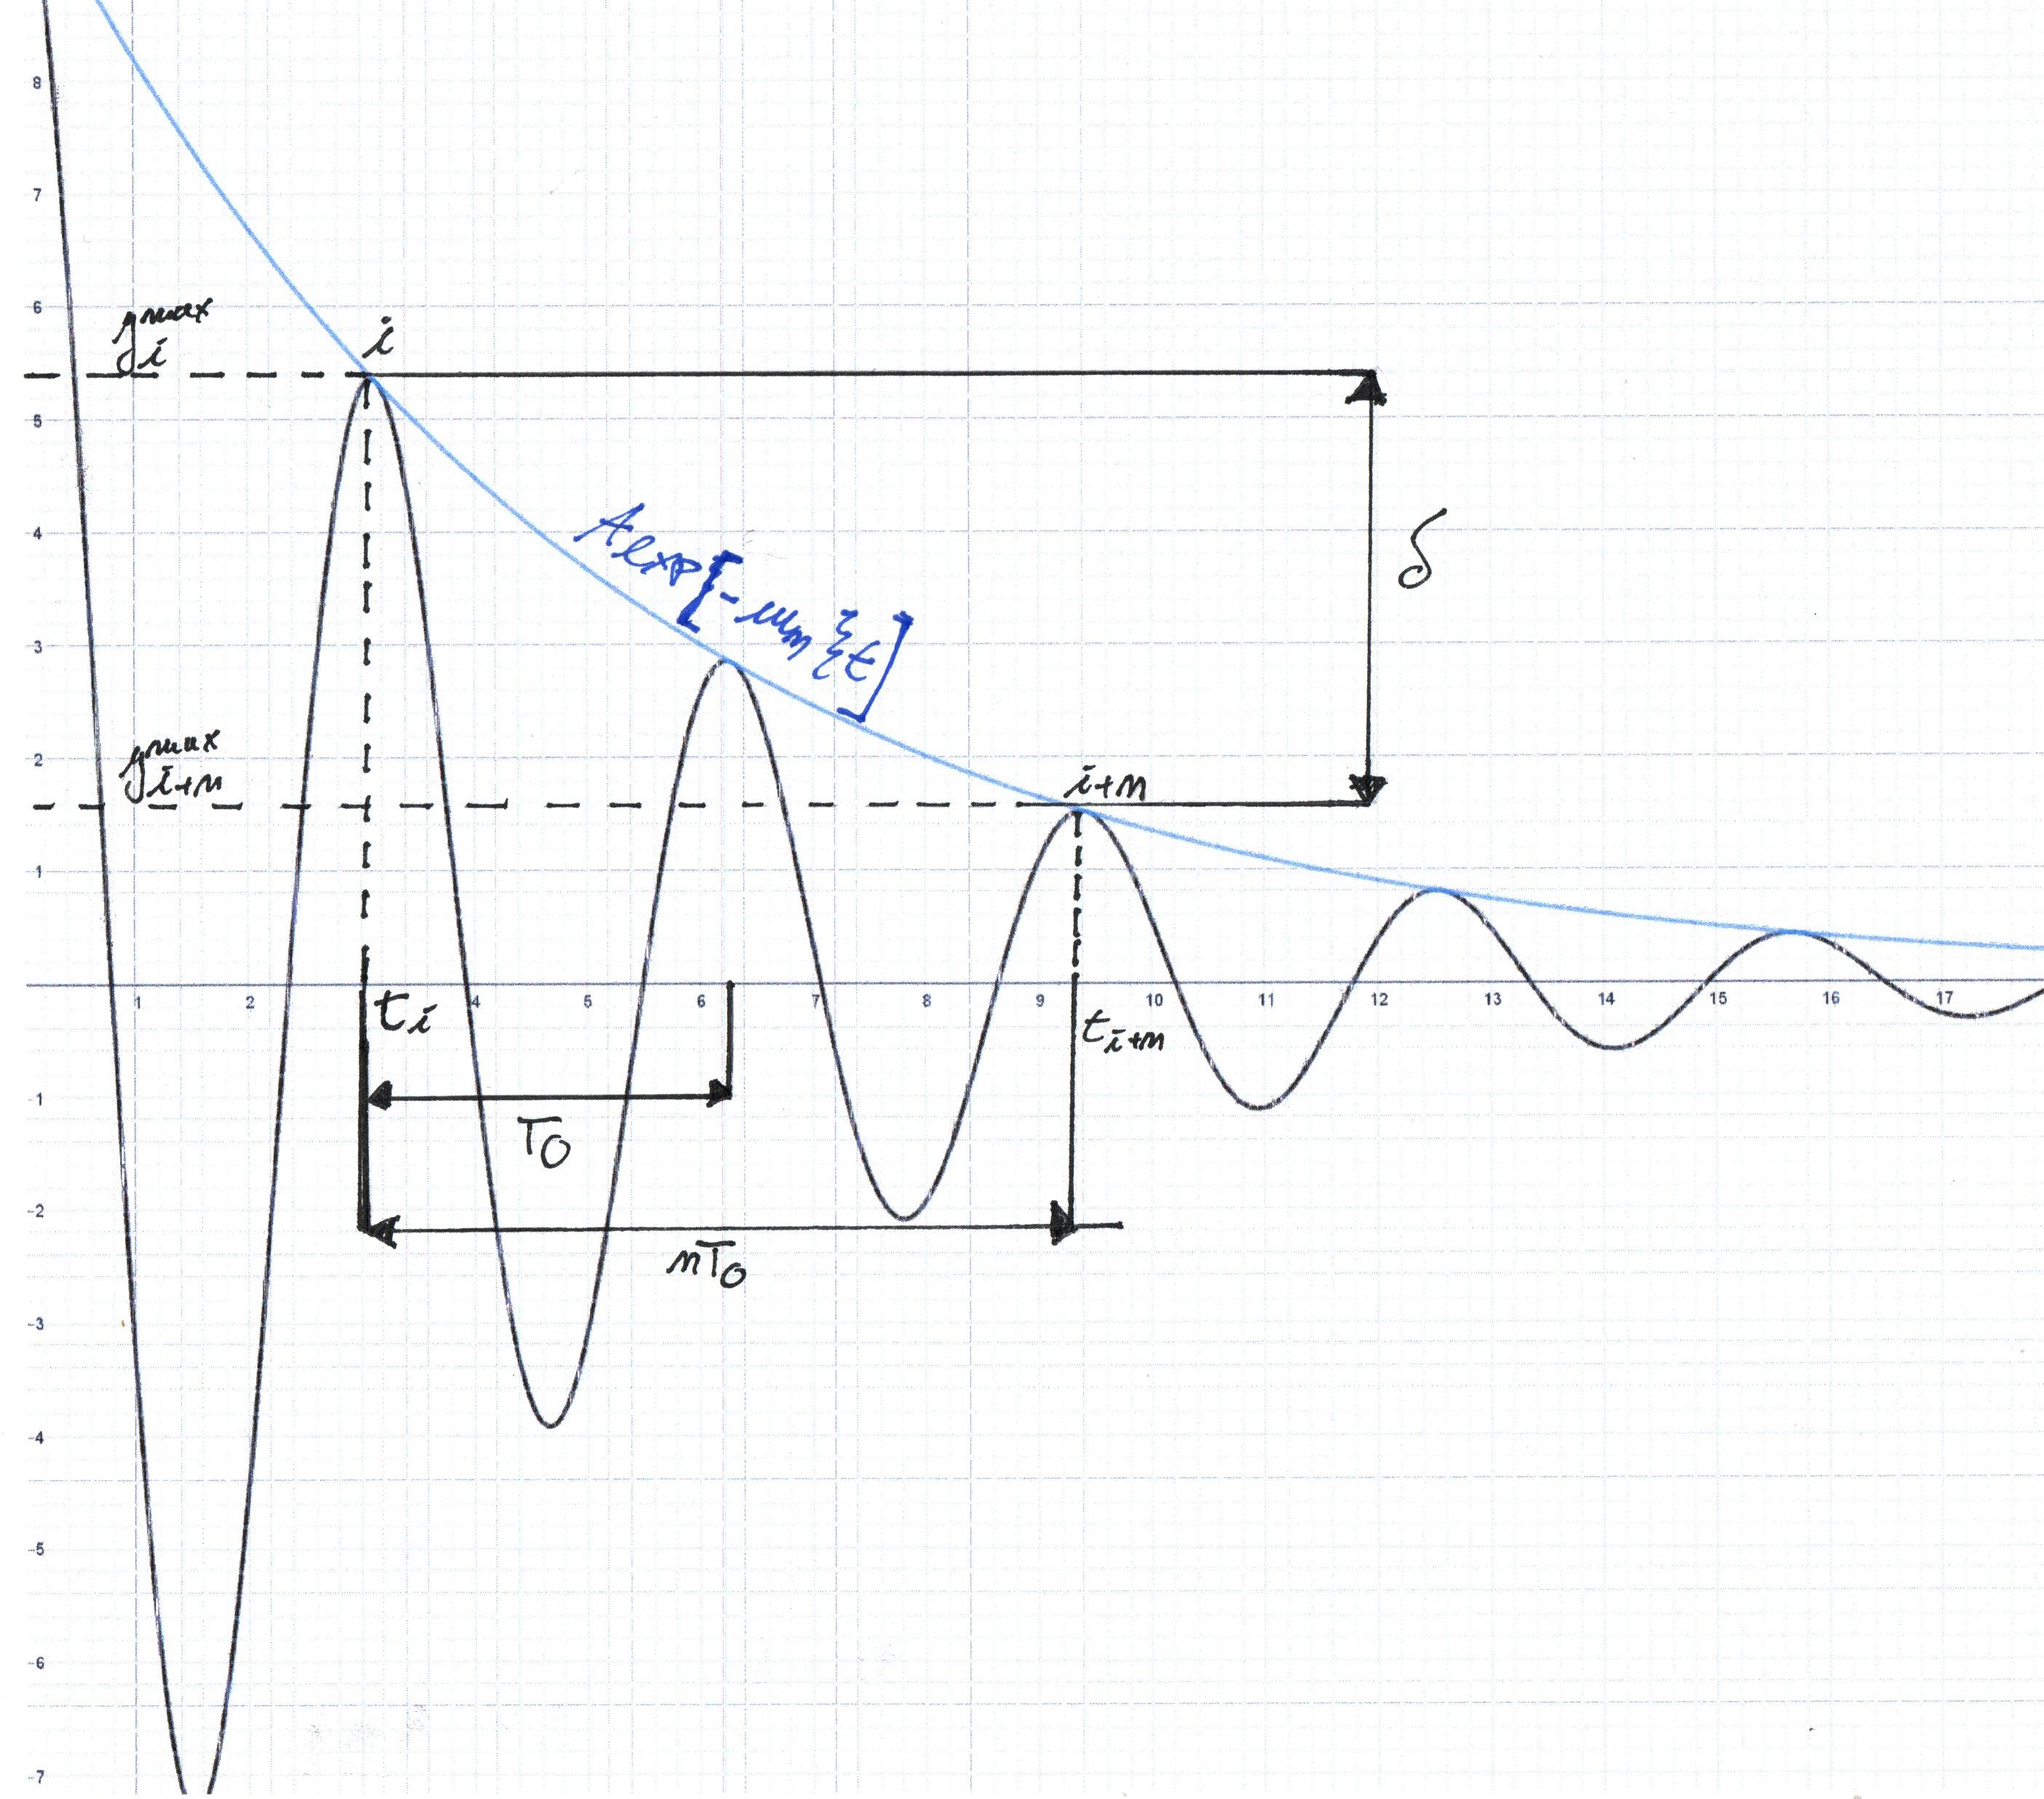
\includegraphics[width=0.5\linewidth]{fig/mm13}
	\label{fig:mm13}
\end{figure}	
	Si definisce decremento logaritmico:
	\[ \delta = {1\over n}\ln\left(\dfrac{y_{M,i}}{y_{M,i+n}}\right)\]
	Graficamente determinabile. \newline 
	
	Matematicamente, equivale a sostituire le rispettive equazioni dei massimi:
	\[ \begin{split}
		\delta & = {1\over n}\ln\left(\dfrac{y_{M,i}}{y_{M,i+n}}\right) =  {1\over n}\ln\left(   \dfrac{Ae^{-\omega_n\xi t_i}}{Ae^{-\omega_n\xi t_{i+n}}}\right) = \\ 
		& = {1\over n}\left(-\xi\omega_nt_i + \xi\omega_nt_{i+n} \right) = {1\over n}\xi\omega_n(t_{i+n} -t_i ) = \\
		& ={1\over n}\xi\omega_n nT_0 = \xi\omega_nT_0 = \xi\omega_n{2\pi\over\omega_0} = \xi\omega_n{2\pi\over \omega_n\sqrt{1 - \xi^2}} = \\
		& \xi{2\pi\over \sqrt{1 - \xi^2}}
	\end{split}\]
	Infine:
	\[ \delta = {2\pi\xi\over \sqrt{1 - \xi^2}} \]
	Conoscendo il $\delta$ attraverso il grafico, possono ricavarmi il $\xi$:
	\[ \xi = \sqrt{\dfrac{\delta^2}{4\pi^2 + \delta^2}}\]
	Nella quale si è implicitamente scelto il segno positivi: $\xi$ dev'essere una grandezza positiva. \newline 
	
	Attraverso la conoscenza di $\delta$ e dopo aver determinato $\xi$, ci si può calcolare $\omega_n$: 
	\begin{eqnarray*}
		\omega_0 = {2\pi\over T_0} = \omega_n\sqrt{1 - \xi^2} = \omega_0  \\
		{2\pi\over T_0} = \omega_n\sqrt{1 - \xi^2}  \\
		\omega_n = {2\pi\over T_0\sqrt{1 - \xi^2}}
	\end{eqnarray*} 
\end{adjustwidth}
%\newpage
\subsection{Gradino crescente} 	
\begin{adjustwidth}{2in}{}	
	Come applico un gradino crescente? Applico una forza istantanea costante, in questo modo l'equazione diviene: 
	\[ M\ddot{y} + c\dot{y} + ky =F_0\]
	Con le seguenti condizioni al contorno:
	\[ \begin{cases}
		y(0) = 0 \\
		\dot{y}(0) = 0
	\end{cases}\]
	La soluzione finale sarà la composizione di una soluzione omogenea (già vista nell'ingresso a gradino decrescente) più una soluzione particolare, quest'ultima col metodo di somiglianza sarà da trovare nella forma di un polinomio di grado uguale a quello a destra dell'uguale, in questo caso: 
	\[y_p = a\]
	Che sostituita nell'equazione di partenza porta a:
	\[[y_p = a = {F_0\over k}\]
	La soluzione particolare sarà quella alla quale tenderà il sistema dopo aver esaurito il transitorio dovuto alla soluzione omogenea. 	
	\begin{figure}[H]
		\centering
		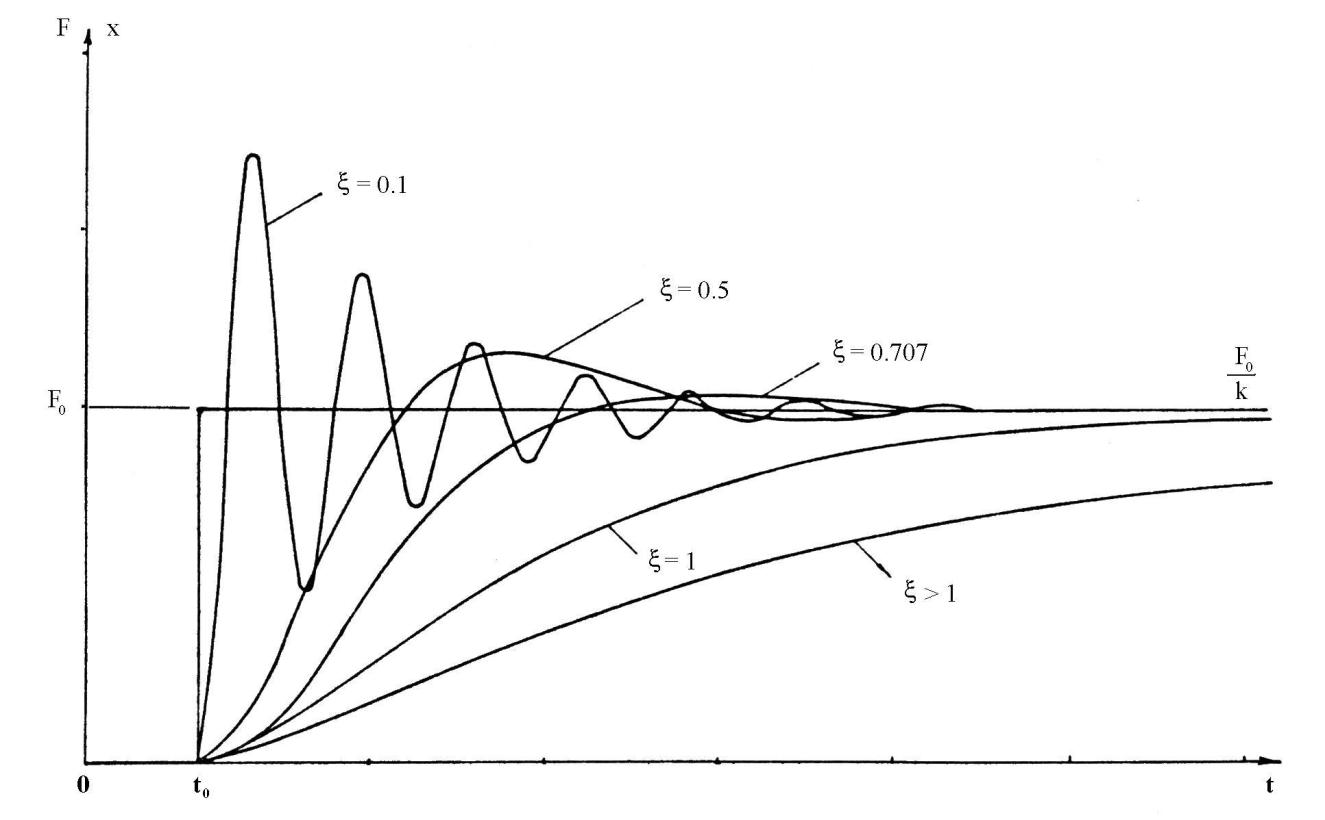
\includegraphics[width=0.7\linewidth]{fig/imag5}
		\label{fig:imag5}
	\end{figure}
	\begin{enumerate}[label=\Roman*.]
	\item \( \xi > 1\) 
	 \[y(t) = A_1e^{\alpha_1 t} + A_2e^{\alpha_2 t} + {F_0\over k} \]
	\item \( \xi = 1 \) 
	\[ \alpha_{1,2} = -\omega_n \hspace{0.5cm} y(t) = A_1e^{-\omega_n t} + A_2te^{-\omega_n t} + {F_0\over k} \]
	\item \( \xi < 1 \) 
	\[\alpha_{1,2} = -\xi\omega_n \pm j\omega_0 \hspace{0.5cm} y(t) = Ae^{-\xi\omega_n t}\sin(\omega_0 t +\varphi) + {F_0\over k} \]	
	In cui alla diminuzione di $\xi$ è associata una diminuzione di periodo. 
	\item\( \xi =0 \) 
	\[ \alpha_{1,2} = \pm j\omega_n \hspace{0.5cm} y(t) = Ae\sin(\omega_n t +\varphi) + {F_0\over k} \]	
	Sinusoide pura.  
\end{enumerate}

	\textbf{NB:}Il massimo è al massimo il doppio del valore di $F_0/k$. \newline 
	
	Si studino le condizioni al contorno della quarta tipologia di funzioni, ideale, senza smorzamento: 
	\[\begin{cases}
		y(t) = Ae\sin(\omega_n t +\varphi) + {F_0\over k} \Rightarrow y(0) = 0 \Leftrightarrow A = -{F_0\over k}\\
		\dot{y}(t) = Ae\omega_n\cos(\omega_n t +\varphi)  \Rightarrow \dot{y}(0) = 0 \Leftrightarrow \varphi = {\pi\over 2}
	\end{cases}\]
	\[y(t) = {F_0\over k} \left[1-\cos(\omega_n t)\right]\]
	Tra quanto varia il termine tra parentesi? tra $0$ e $2$, il che vorrà dire che gli $y$ potranno variale al massimo tra $0$ e $2{F_0/k}$. \newline
	
	Similmente a quanto fatto per il gradino decrescente, anche in questa occasione la miglior scelta di $\xi$ rimane quella per cui: 
	\[ \xi = 0.7 \]
	
	\textbf{NB:} Per il calcolo del decremento logaritmico si fa riferimento alle quote dei massimi traslate ora rispetto all'asintoto, e non a $0$ come nel gradino decrescente.  
\end{adjustwidth}
%\newpage
\subsection{Rampa} 	
\begin{adjustwidth}{2in}{}	
	Caratterizzato da una forza linearmente dipendente dal tempo:
	\[ M\ddot{y} + c\dot{y} + ky =f_0t\]
	Anche qui la soluzione particolare si andrà a cercare nella forma di un polinomio con lo stesso grado della funzione nota, per cui:
	\[ y_p = a + bt\]
	Che sostituita porta ad avere:
	\[ cb + ka + kbt = f_0t\]
	Il metodo di somiglianza sancisce che: 
	\[ \begin{dcases}
		kb = f_0 \Rightarrow b = {f_0\over k} \\
		cb + ka = 0 \Rightarrow a = -{c\over k}{f_0\over k}
	\end{dcases}\]
	Ricordi come ${c\over k}$ fosse uguale al $\tau_r$ di ritardo? \newline 
\newpage	
	La soluzione particolare che questo ingresso produrrà sarà: 
	\[ y_p = {f_0\over k}(t-\tau_r)\]
\begin{figure}
	\centering
	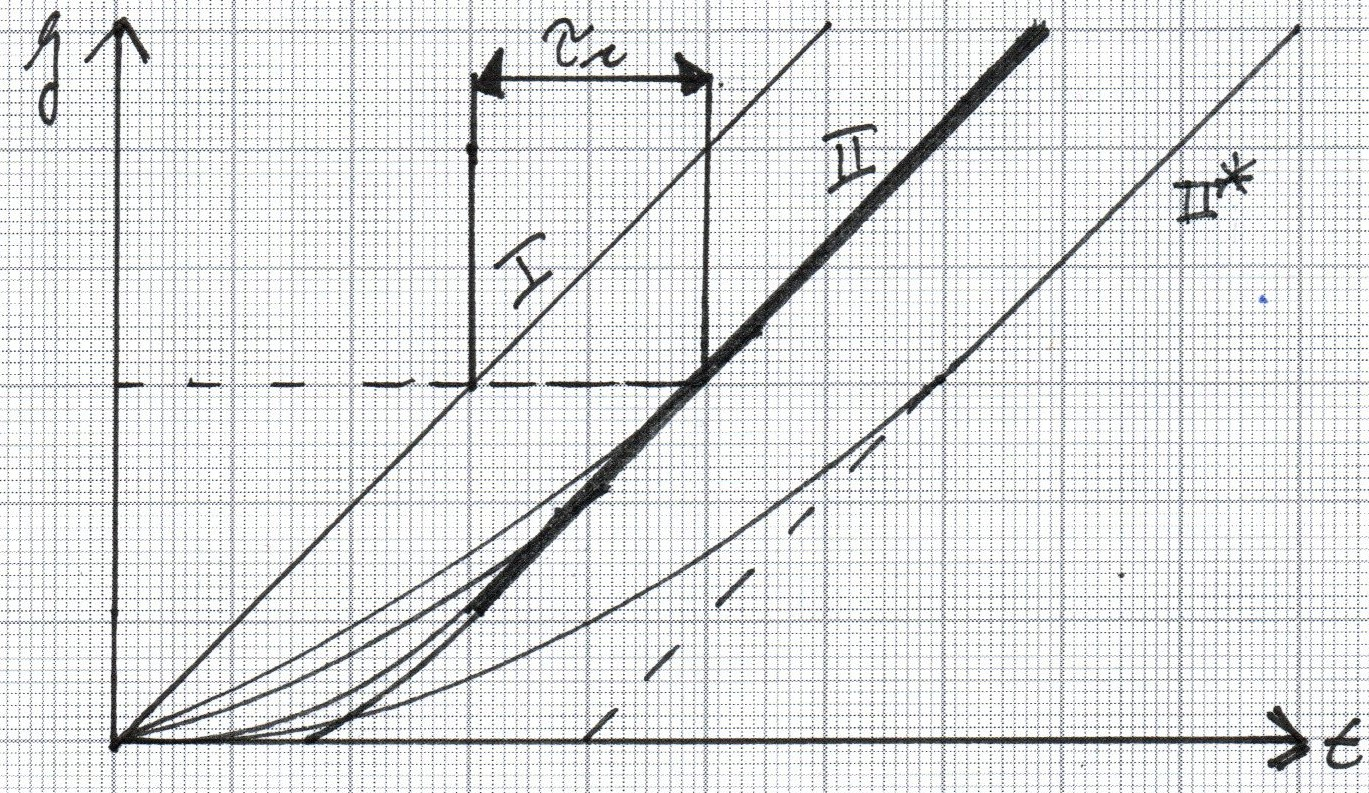
\includegraphics[width=0.5\linewidth]{fig/mm14}
	\label{fig:mm14}
\end{figure}
\begin{enumerate}[label=\Roman*.]
		\item \(\xi > 1\) è caratterizzato dallo stesso andamento dello strumento del primo ordine, una partenza esponenziale con tendenza ad un valore asintotico in ritardo rispetto al valore ideale/teorico. 
		\item \(\xi >> 1\) è caratterizzato da un'esponenziale più lenta. 
		\item[II*.] \(\xi >> 1\), sottocaso del precedente in cui si può ottenere addirittura la traslazione dell'asintoto: 
		\[\tau_r = {c\over k} \hspace{1cm} \xi = \dfrac{c}{2\sqrt{kM}}\]
		Come ottengo uno $\xi$ elevato? (perchè lo dovrei ottenenre?)
		
		Diminuendo la massa, $\xi$ varia e $\tau_r$ rimane invariato, agendo invece su $k\downarrow$ e $c\uparrow$, oltre a far variare $\xi$ ottengo una variazione di $\tau_r$, e dunque una traslazione dell'asintoto.
		\item \(\xi = 1\) si ottiene la curva che più delle altre tende più rapidamente all'asintoto.
		\item \(\xi < 1\), si ottiene una curva come in figura seguente. 		
\begin{figure}[H]
	\centering
	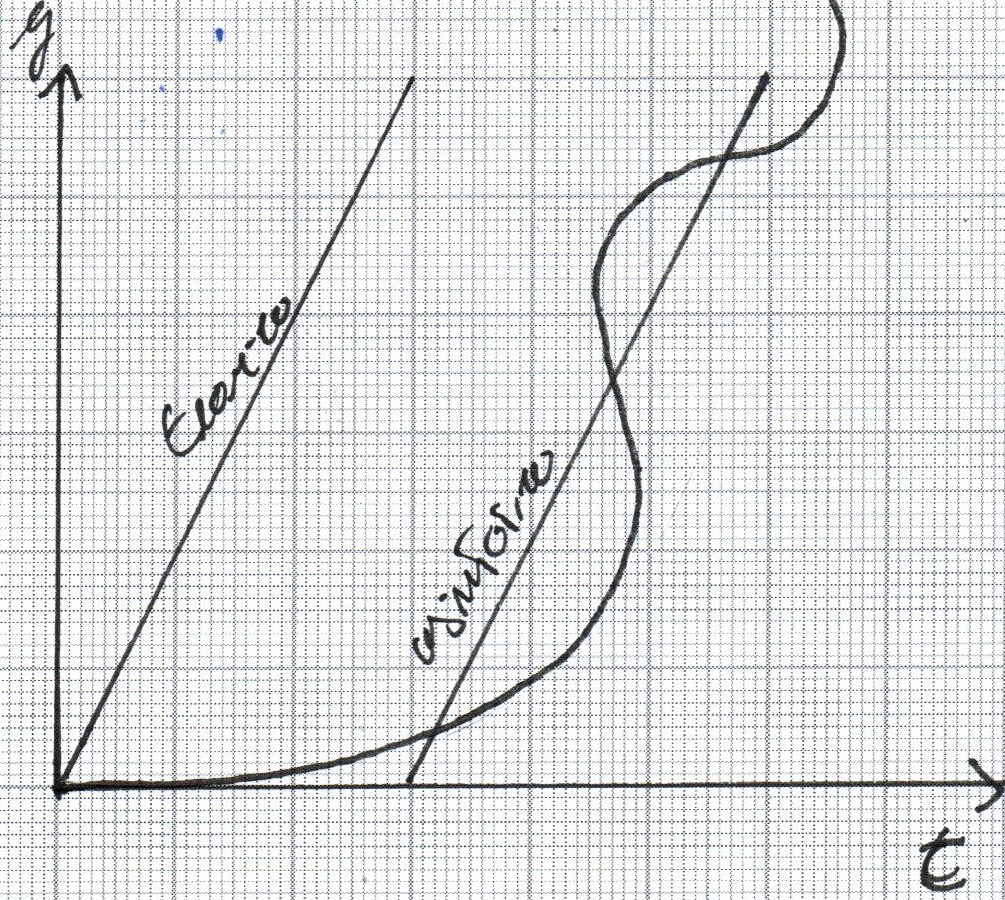
\includegraphics[width=0.3\linewidth]{fig/mm15}
	\label{fig:mm15}
\end{figure}
\end{enumerate}
\end{adjustwidth}
\newpage
\subsection{Ingressi periodici} 	
\begin{adjustwidth}{2in}{}
			Si ottiene applicando una forza sinusoidale. 
			\[ M\ddot{y} + c\dot{y} + ky =F_0\sin\omega t\]
			Così come effettuato negli strumenti del primo ordine, si visualizzeranno con questo ingresso i grafici del guadagno e delle pulsazioni/frequenza. 
			
			Sempre come effettuato con gli strumenti del primo ordine, si trascurerà la soluzione omogenea caratteristica del transitorio dello strumento e ci si concentrerà sulla soluzione a regime fornita da quella particolare. \newline
			
			Si passerà sempre attraverso il metodo simbolico
			\[ M\ddot{y} + c\dot{y} + ky =F_0e^{j\omega t}\]
			La soluzione particolare sarà data nella forma: 
			\[ y_p = y_0e^{j\omega t}e^{j\varphi}\]
			Che sostituita porta a:
			\[\begin{split} 
				-M\omega^2y_0e^{j\omega t}e^{j\varphi} + cj\omega y_0e^{j\omega t}e^{j\varphi} + ky_0e^{j\omega t}e^{j\varphi} & =F_0e^{j\omega t} \\
				-M\omega^2y_0e^{j\varphi} + cj\omega y_0 e^{j\varphi} + ky_0e^{j\varphi} & =F_0 \\
				y_0e^{j\varphi}\left(-\omega^2M + jc\omega + k\right) & = F_0 \\
				y_0e^{j\varphi}\left(-\omega^2{M\over k} + j\omega{c\over k}  + 1\right) & = {F_0\over k} 	
			\end{split} \]
			Ricordando che:
			\[c = 2\sqrt{kM}\xi \hspace{1cm} \sqrt{k\over M}\]
			Si giunge a
			\[
			\begin{split}
				y_0e^{j\varphi}\left[-\left({\omega\over \omega_n}\right)^2 + j\omega{2\sqrt{kM}\xi\over k}  + 1\right] & = {F_0\over k} 	\\
				y_0e^{j\varphi}\left[-\left({\omega\over \omega_n}\right)^2 + j2\xi{\omega\over \omega_n}  + 1\right] & = {F_0\over k} 	\\
				y_0e^{j\varphi}\left[1-\left({\omega\over \omega_n}\right)^2 + j2\xi{\omega\over \omega_n}\right] & = {F_0\over k}
			\end{split}
			\]
			Ottenendo così che:
			\[ y_0e^{j\varphi} = {F_0\over k} \dfrac{1}{1-\left({\omega\over \omega_n}\right)^2 + j2\xi{\omega\over \omega_n}} \]
			Come per gli strumenti del primo ordine razionalizzo per ottenere un numero complesso dal quale ricavare un modulo ed una fase:
			\[ {F_0\over k} \dfrac{1}{1-\left({\omega\over \omega_n}\right)^2 + j2\xi{\omega\over \omega_n}} \cdot \dfrac{1-\left({\omega\over \omega_n}\right)^2  j2\xi{\omega\over \omega_n}}{1-\left({\omega\over \omega_n}\right)^2 - j2\xi{\omega\over \omega_n}}\]
			\[ y_0e^{j\varphi} = {F_0\over k} \dfrac{1-\left({\omega\over \omega_n}\right)^2 - j2\xi{\omega\over \omega_n}}{\left[1-\left({\omega\over \omega_n}\right)^2\right]^2 + \left(2\xi{\omega\over \omega_n}\right)^2} \]
			Il modulo è dato da: 
			\[ y_0 = {F_0\over k} \dfrac{\sqrt{\left[1- \left(\omega\over\omega_n\right)^2\right]^2 + 4\xi^2\left(\omega\over\omega_n\right)^2}}{\left[1-\left({\omega\over \omega_n}\right)^2\right]^2 + 4\xi^2\left(\omega\over\omega_n\right)^2} \]
			Infine:
			\[ y_0 = {F_0\over k} \dfrac{1}{\sqrt{\left[1- \left(\omega\over\omega_n\right)^2\right]^2 + 4\xi^2\left(\omega\over\omega_n\right)^2}}\]
			E la fase sarà data da: 
			\[ \varphi = \arctan\left[\dfrac{-2\xi \omega/\omega_n}{1-(\omega/\omega_n)^2}\right]\]
			Si ottiene un grafico del guadagno dipendente sia da $xi$ che da $\omega_n$: 			
\begin{figure}[H]
	\centering
	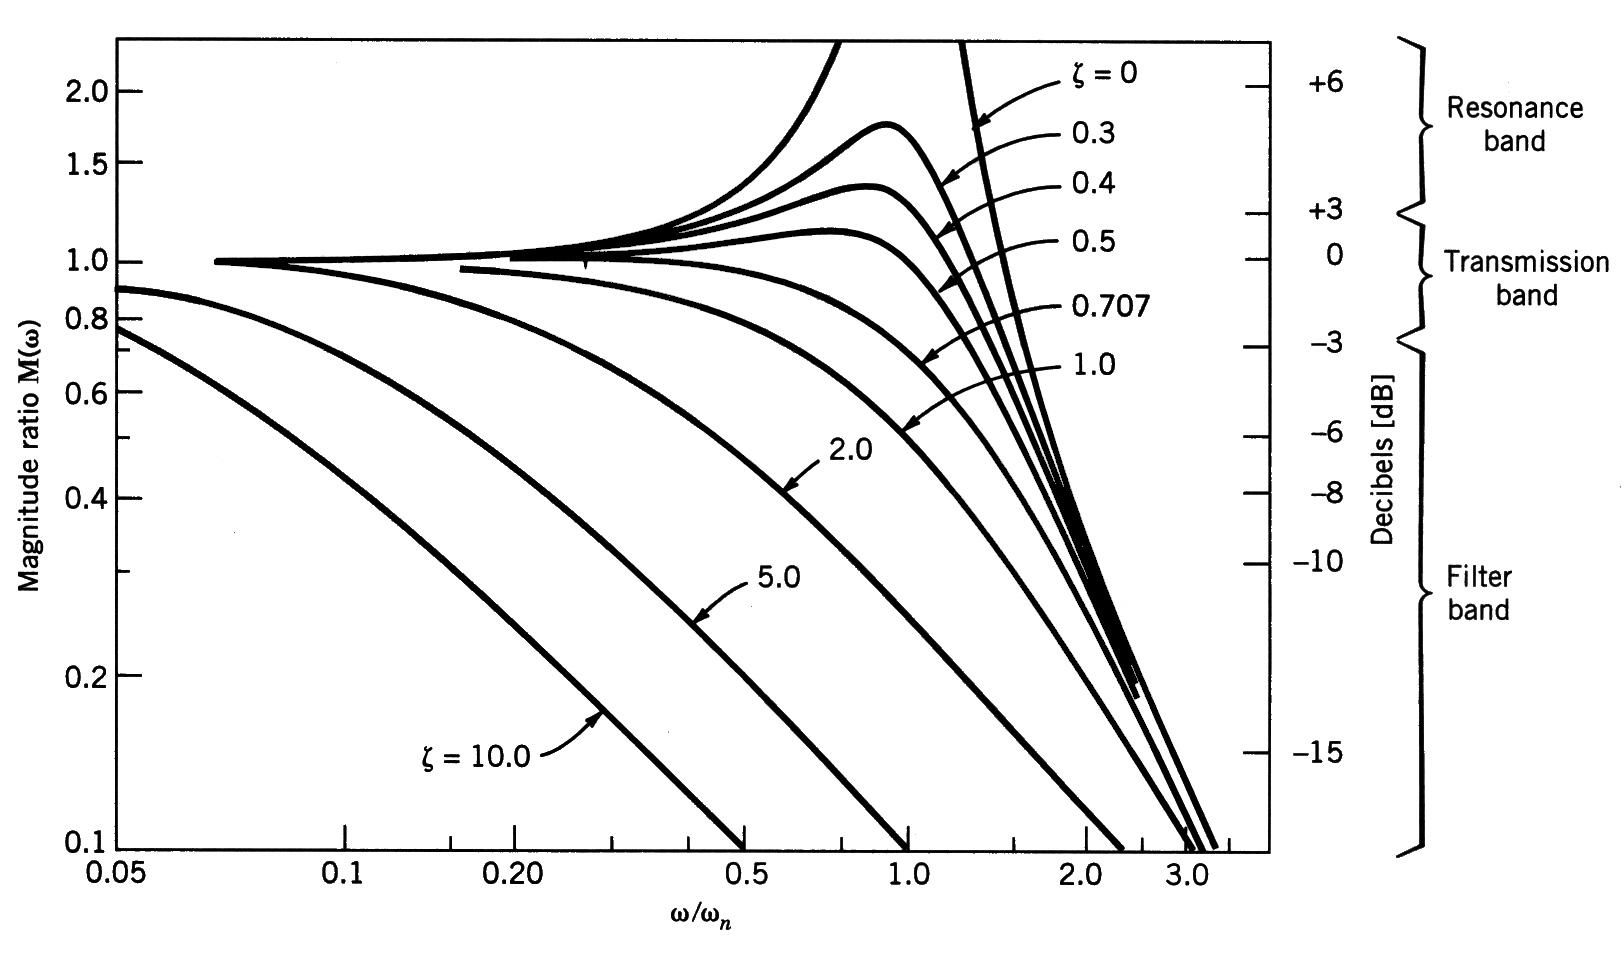
\includegraphics[width=0.7\linewidth]{fig/imag6}
	\label{fig:imag6}
\end{figure}
			Dove a \(\omega = 0 \qquad y_0 = {F_0\over k}\): a segnale costante corrisponde valore massimo, idealmente. \newline
			
			Per \(\omega\rightarrow\infty \qquad y_0 \rightarrow 0\). \newline
			
			Per \( \omega = \omega_n \qquad y_0 = \dfrac{F_0}{k}\dfrac{1}{2\xi} \), su questa ordinata, si possono identificare i seguenti casi:
			\begin{itemize}
				\item Se \(\xi >> 1 \hspace{0.5cm} y_0 \rightarrow0\);
				\item Se \(\xi = 1 \hspace{0.5cm} y_0 = \dfrac{1}{2}\dfrac{F_0}{k}\);
				\item Se \(\xi = {1\over 2} \hspace{0.5cm} y_0 \approx \dfrac{F_0}{k}\);
			\end{itemize}
			Al diminuire della frequenza so salendo di quota sull'ascissa prefissata, cosa succede per l'unico caso che non si è trattato? Cosa succede se \(\xi = 0\)?
			Avviene una discontinuità: se \(\xi =0 \hspace{0.5cm} y_0 \rightarrow\infty\), sto dando una sinusoide la cui frequenza è pari a quella naturale del sistema, sto dando la frequenza di risonanza. 
			
			Per progettare uno strumento è necessario stare ben alla larga dalla frequenza di risonanza.
			
			Anche qui la miglior scelta rimane quella di avere uno smorzamento pari a
			\[\xi = 0.7\] 
\end{adjustwidth}
\newpage
\subsubsection{Frequenza di taglio \& grafico della fase} 	
\begin{adjustwidth}{2in}{}
			Questa è definita come
			\[ f_t \coloneqq -3dB = 20\log\left[\dfrac{y_0(f_t)}{y_0(0)}\right]\]
			Ovvero quella frequenza alla quale si ha una deamplificazione di $3dB$ data da un rapporto dove al numeratore compare il guadagno alla frequenza di taglio e al denominatore il guadagno a frequenza costante, nulla, ideale. 
			\[  -3dB = 20\log\underbrace{\left[ \dfrac{1}{\sqrt{\left[1- \left(\omega\over\omega_n\right)^2\right]^2 + 4\xi^2\left(\omega\over\omega_n\right)^2}}\right]}_\text{$=0.7$}\]
			Ne consegue che la frequenza di taglio si avrà per una deamplificazione del segnale del $30\%$.
			
			Importante notare come la frequenza di taglio sia dipendente da $\xi$ ed $\omega_n$. \newline 
			
			La banda passante sarà così:
			\[BP = [0, f_t]\]
			Logico che se vorrò avere una frequenza maggiore del segnale in ingresso, bisognerà avere una banda passante maggiore.\newline
			
			\textbf{In che modo aumento la banda passante? Diminuendo $\xi$.}
			
			Attenzione però a ridurlo troppo, in questo modo la frequenza di taglio torna indietro, presentando un segnale ora crescente che incontrando prematuramente la frequenza di taglio ne abbassa la banda, la curva esce subito, mentre va mantenuta il più possibile all'interno della banda passante. \newline 
			
			\textbf{Come scelgo ora il valore di $\omega_n = \sqrt{k\over M}$?}
			
			Innanzitutto con $\omega_n$ elevato la banda passante cresce riuscendo ad ottenere uno strumento dalla dinamica più rapida, ed in secondo luogo, è bene rimanere distanti dalla pulsazione naturale per evitare fenomeni di risonanza potenzialmente distruttivi, un $\omega_n$ basso in aggiunta ad uno $\xi$ elevato permetterebbe di far passare all'interno della banda passante anche la frequenza di risonanza. \newline 
			
			Il grafico della fase si ottiene imponendo all'equazione della fase i valori \[\omega = \omega_n, 0, \infty\]
			
			Disegnando poi il grafico per vari $\xi$ si incontra in $\xi=0$ una discontinuità di salto.			
\begin{figure}[H]
	\centering
	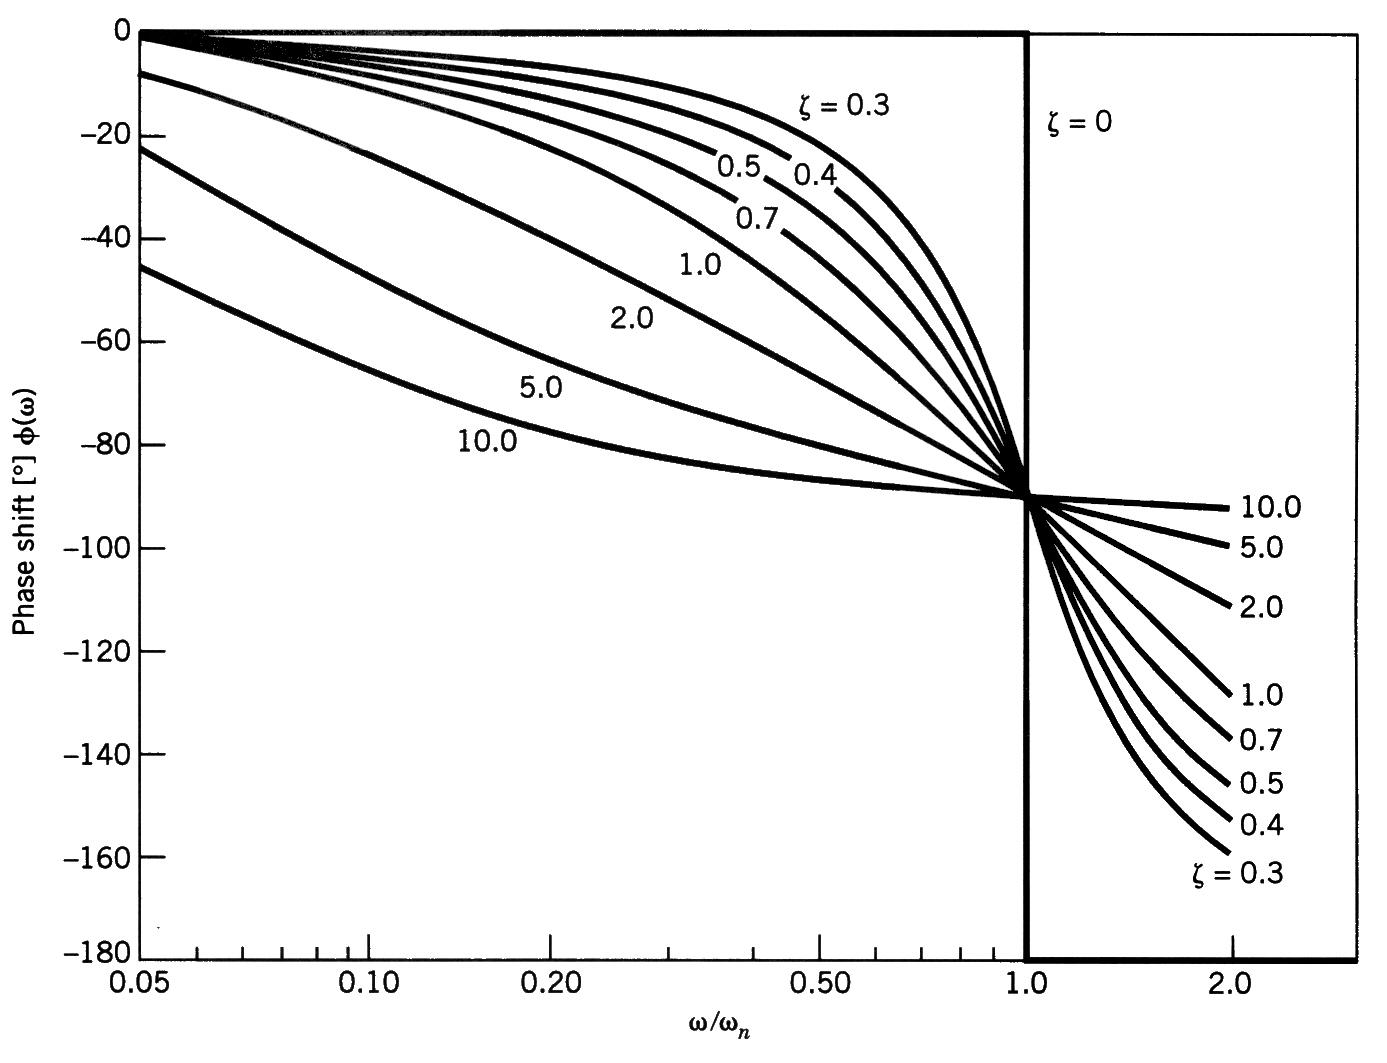
\includegraphics[width=0.5\linewidth]{fig/imag7}
	\label{fig:imag7}
\end{figure}
\end{adjustwidth}
\newpage
\subsubsection{Galvanometro/Amperometro} 	
\begin{adjustwidth}{2in}{}
		Tale strumento riceve in input una corrente che trasforma, attraverso lo schema di seguito, in una variazione angolare su di un display. 		
\begin{figure}[H]
	\centering
	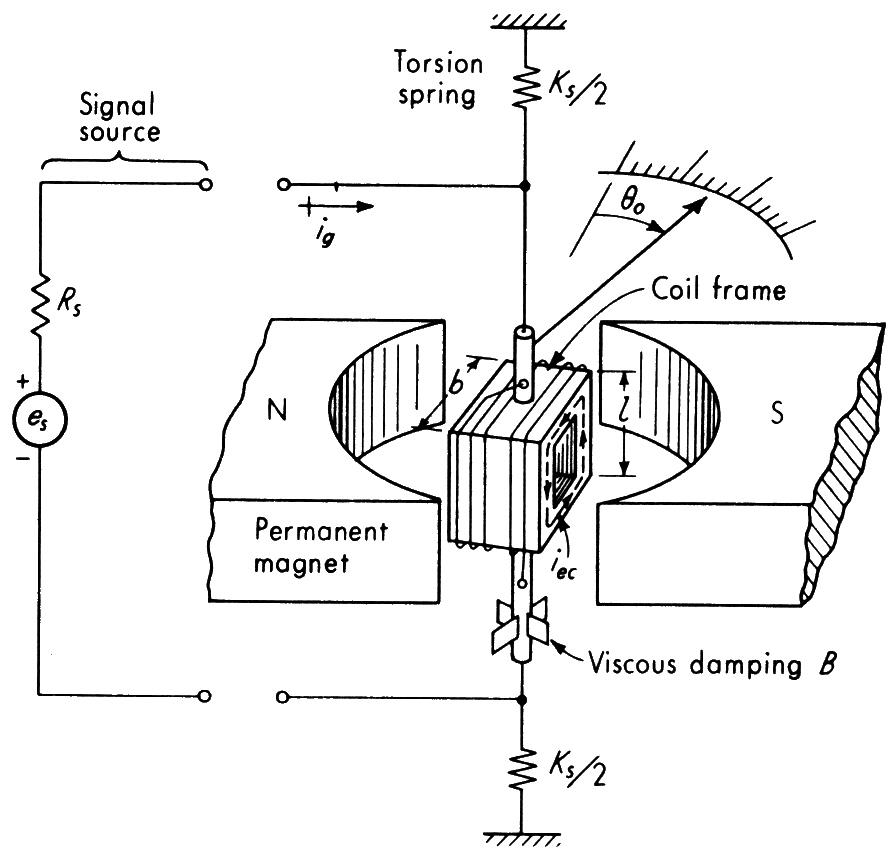
\includegraphics[width=0.3\linewidth]{fig/imag8}
	\label{fig:imag8}
\end{figure}
		Un nucleo ferromagnetico avvolto di spire è posto tra un campo magnetico, il nucleo ruoterà a causa della corrente che percorrendo le spire genererà un momento magnetico mentre due molle torsionali che fissano il nucleo al telaio manterranno il nucleo in sede. Un indicatore solidale al nucleo indicherà l'angolo di rotazione. \newline 
		
		L'equazione che governa il moto è:
		\[F = i\vec{l}\times \vec{B}\]
		Più spire in un campo magnetico uniforme imposto generano un momento di rotazione dato da:
		\[ M = n\cdot ilbB\]
		Bene notare che l'unica grandezza qui a variare è la corrente, oggetto di misura, il campo magnetico è imposto e noto. \newline 
		
		Da cosa sarà impedita la rotazione della spira? Dalle molle torsionali solidali al telaio che applicheranno un momento pari a: 
		\[M=k\theta\]
		Avremo perciò l'uguaglianza: 
		\[ n\cdot ilbB = k\theta \Rightarrow \theta = \dfrac{lbnB}{k}i\]
		E la sensibilità è data da:
		\[ S = \dfrac{lbnB}{k} \]
		Che legge dinamica è espressa dallo strumento? Ricordando che per un corpo in rotazione entra in gioco il momento d'inerzia $I$ dello specifico oggetto, si avrà:
		\[I\ddot{\theta} + c\dot{\theta} + k\theta = M\]
		Alla quale si associano pulsazione naturale e fattori di smorzamento dati da: 
		\[ \omega_n = \sqrt{k\over I} \hspace{1cm} \xi = \dfrac{c}{2\sqrt{kI}}\]
		Come si vede, ad esempio un aumento di $k$, che porterebbe ad un aumento di $\omega_n$, porta ad una diminuzione di $S$: le caratteristiche metrologiche statiche sono ancora in disaccordo con quelle dinamiche. 

			 
		\newpage
		
		{\LARGE \textbf{NOTE}}	
			
	
	
	
	
	
	
	
	
	
	
	
	
	
	
	
	
	
	
	
	
	
	
	
	
	
	
	
	
	
	
	
	
	
	
	
	
	
	
	
	
	
	
	
	
	
	
	
	
	
	
	
	
	
	
	
	
	
	
	
	
	
	
	
	
	
	
	
	
	
	
	
	
	
	
	
	
	
	
	
	
	
	
	
	
	
	
	
	
	
	
	
	
	
	
	
	
	
	
	
	
	
	
	
	
	
	
	
	
	
	
	
	
	
	
	
	
	
	
	
	
	
	
	
	
	
	%DA DECOMMENTARE PER AVERE LA VERSIONE STAMPABILE A DUE PAGINE 	
	%	\newpage
	%		\null
	%		\vfill
	%\begin{tcolorbox}[height=4.5cm]
	%	This box has a height of 4.5cm.
	%\end{tcolorbox}
	%		
\end{adjustwidth}
\end{document}